\documentclass[12pt]{aghdpl}
% \documentclass[language=en,11pt]{aghdpl}  % praca w języku angielskim

%---------------------------------------------------------------------------

\author{Mateusz Strzałkowski}
\shortauthor{M. Strzałkowski}


\titlePL{\huge{ Heterodoksyjnie proceduralny język programowania i jego kompilator.}}
\titleEN{\large{Heterodoxically procedural programing language and its compiler.}}


\shorttitlePL{Heterodoksyjnie proceduralny język programowania i jego kompilator.} % skrócona wersja tytułu jeśli jest bardzo długi
\shorttitleEN{Heterodoxically procedural programing language and its compiler.}


% Dopuszczalne wartości[1,2]:
% * "Projekt dyplomowy" - na koniec studiów I stopnia
% * "Praca dyplomowa" - na koniec studiów II stopnia
% [1] Zasady dyplomowania w roku akademickim 2020/2021 (Decyzja Dziekana WEAIiIB nr 16/2020 z dnia 9 grudnia 2020 roku)
% [2] Załącznik nr 1a) do Decyzji nr 16/2020 Dziekana Wydziału EAIiIB z dnia 09 grudnia 2020 r.
\thesistype{Projekt dyplomowy}
%\thesistype{Master of Science Thesis}

\supervisor{dr Dariusz Pałka}

\degreeprogramme{Informatyka i systemy inteligentne}
%\degreeprogramme{Automatics and Robotics}

\date{2024}

%\department{Katedra Informatyki Stosowanej}
%\department{Department of Applied Computer Science}

\faculty{Wydział Elektrotechniki, Automatyki, Informatyki i Inżynierii Biomedycznej}
%\faculty{Faculty of Electrical Engineering, Automatics, Computer Science and Biomedical Engineering}

\acknowledgements{Serdecznie dziękuję promotorowi, panu Terence Parrowi (za antlr) oraz autorom projektu LLVM}

\definecolor{mygreen}{rgb}{0,0.6,0}
\definecolor{mygray}{rgb}{0.5,0.5,0.5}
\definecolor{mymauve}{rgb}{0.58,0,0.82}

\lstset{ %
  backgroundcolor=\color{white},   % choose the background color
  basicstyle=\footnotesize,        % size of fonts used for the code
  breaklines=true,                 % automatic line breaking only at whitespace
  captionpos=b,                    % sets the caption-position to bottom
  %commentstyle=\color{mygreen},    % comment style
  escapeinside={\%*}{*)},          % if you want to add LaTeX within your code
  %keywordstyle=\color{blue},       % keyword style
  %stringstyle=\color{mymauve},     % string literal style
}
\begin{document}

	\titlepages
	\RedefinePlainStyle
	
	\setcounter{tocdepth}{2}
	\tableofcontents
	\clearpage
	
	\chapter{Wstęp}
\label{cha:wstep}

Wobec mnogości i różnorodności dostępnych obecnie języków programowania, zaskoczeniem może się wydać, że istnieją pewne koncepcje językowe nigdy nie zrealizowane, bądź historycznie wypróbowane, a dziś nieobecne. W niniejszej pracy rozwinięty zostanie nowy proceduralny język programowania, wykorzystujący i łączący kilka interesujących form lingwistycznych.
Urzeczywistni się ten język poprzez program jego automatycznego translatora dla maszyn cyfrowych. Możliwość i poziom trudności skonstruowania praktycznie użytecznego kompilatora nowego języka, dysponując ograniczonymi zasobami, lecz korzystając ze współczesnych narzędzi w sposób poparty ugruntowanymi osiągnięciami lingwistyki formalnej, będzie również kluczowym przedmiotem badań.

%---------------------------------------------------------------------------

\section{Czy nowe języki programowania są potrzebne?}
Języki ,,wysokiego poziomu'', które dziś odpowiadają powszechnemu pojęciu o "językach programowania" pojawiły się w latach sześćdziesiątych(pięćdziesiątych??) ubiegłego wieku. Wydawać by się mogło, że od tego czasu, problem, na jaki stanowiły odpowiedź - zapewnienie zrozumiałego zarówno dla człowieka jak i maszyny opisu algorytmu, po tylu dekadach doczekał się zadowalających rozwiązań - innymi słowy zaproponowano i przetestowano większość wartych uwagi możliwości i dostępne obecnie języki programowania są co najmniej wystarczające i pole do usprawnień pozostaje niewielkie.
Zdaje się mieć to odzwierciedlenie w spadającej w ostatnich latach liczbie języków nowych - takich, które zyskały publiczne uznanie i grono użytkowników[VALVERDE 2016, ...]. Powodem może być pewna dojrzałość wypracowana przez najpopularniejsze obecnie języki oraz osiągnięcie przez nie takiego poziomu abstrakcji, na którym problemy niegdyś modelowane przez specjalnie określone struktury syntaktyczne, oddać można za pomocą istniejącej, dużo ogólniejszej składni.
Przykładem niech będzie obsługa dostępu do plików w języku PL/I popularnym w latach 70, gdzie istniał dedykowany aparat w składniowy, zawierający np. osobne słowo kluczowe FILE. We współczesnym C++, czy Javie, w specyfikacji języka próżno szukać przeznaczonych do tego konstrukcji. Operacje na plikach realizowane są poprzez funkcjonalności bibliotek standardowych i nie wymagają modyfikacji języka.
Wydawać by się mogło, że po osiągnięciu pewnego poziomu abstrakcji syntaktycznej (w szczególności typów parametryzowanych), innowacje mogą ograniczyć się do rozszerzania leksykonu języka, nie modyfikując składni. Poniższy przykład, wzięty z bardzo obecnie rozpowszechnionej praktyki programistycznej ma za zadanie podważyć to twierdzenie i zwrócić uwagę na złożoność relacji pomiędzy składnią a leksykonem języka.

Napisana w Javie biblioteka Spring nie jest pierwszym i z pewnością nie ostatnim podejściem do stworzenia ekosystemu ułatwiającego tworzenie serwerów i złożonych aplikacji sieciowych. Najtrafniejszym jej określeniem pozostanie jednak "framework", ponieważ nie stanowi ona jedynie zbioru procedur gotowych do użycia, jak biblioteka, a określa również szkielet aplikacji i do pewnego stopnia redefiniuje sposób pisania programu, teoretycznie wciąż w języku Java. Niech zademonstruje to poniższy wycinek:
\begin{lstlisting}[language=java]
@Stateless
@Resource
@Auth
public class CarResource{
    @Autowired private CarService service;

    @Permission(Perm.CarR)
    @GetMapping("/cars")
    GetCarsResponse getCars(GetCarRequest request){
        return service.availableCars(getFilters(request));
    }
    ...
    @Permission(Perm.CarRW)
    @PostMapping("/cars")
    ReserveCarResponse reserveCar(String){...}
}
\end{lstlisting}

Pierwszą obserwacją niech będzie, że człowiek zaznajomiony jedynie ze specyfikacją języka Java marne ma szanse zrozumienia powyższego wycinka programu. Jeśli orientuje się w zagadnieniach sieciowych, zna pojęcie REST API i programowanie zorientowane obiektowo, może zrozumieć już bardzo wiele, potencjalnie cały zamysł programu, umknąć mu jednak mogą kluczowe szczegóły. Na przykład, zakładając, że reserveCar dokonuje modyfikacji w bazie danych, ów programista mógłby zacząć zadawać pytania o zachowanie systemu w wypadku błędu wewnątrz procedury rezerwującej samochód. Jeśli nie jest przeszkolonym użytkownikiem Springa, nie ma sposobu aby domyślił się, że jednym z efektów oznaczenia klasy jako @Stateless, jest „opakowanie” kodu każdej metody tej klasy nową transakcją baozodanową (jeśli takowej wcześniej nie rozpoczęto) i odwinięcie jej w wypadku wystąpienia wyjątku podczas wykonania kodu wewnątrz, a jest to szczegół o potencjalnie kluczowym znaczeniu dla analizy programu. [Spring @Stateless, transaction propagation RequiresNew itd]
Do jakiego stopnia jest zatem ów program napisany w Javie, do jakiego stopnia w Springu? Czy Spring jest jeszcze biblioteką, frameworkiem, czy może raczej osobnym językiem? Fakt, że ów język pozostaje podzbiorem Javy i jest wciąż tłumaczony przez jej kompilator ma jednak swoją cenę. 
Java jest w założeniach językiem kompilowanym i statycznie typowanym. Zapewniać ma to bezpieczeństwo typów, wymuszane podczas tłumaczenia programu. Poniższa linia:
    CarService service = new CarService(carRepository);
nie powinna pozostawiać pola dla wielu niespodzianek podczas wykonania, gdy zostanie pomyślnie skompilowana.
Jeśli programista zapomni dopisać klasę CarSevice, bądź ją zaimportować aby była widoczna w tym pliku (jednostce translacji), od razu otrzyma błąd kompilacji.
Konstrukcja springowa będąca jej odpowiednikiem:
@Autowired private CarService service;
nie zapewnia nawet tych prostych gwarancji. W podstawowym przypadku, gdy CarService fizycznie nie istnieje, faktycznie, tak samo nazwa nie zostanie odnaleziona w zakresie. Gdyby jednak wstrzykiwany obiekt był interfejsem np., 
@Autowired ICarService service; 
(w innym miejscu:)CarService implements ICarService
albo typem parametryzowanym (w nomenklaturze Javy - generycznym)
@Autowired PageableService<Car> service; 
(w innym miejscu: )CarService extends PageableService<Car>,
program mógłby się skompilować i dopiero przy jego uruchomieniu wystąpiłby błąd - maszyneria Springa mogłaby nie móc odnaleźć (np. z powodu błędnej konfiguracji) odpowiedniej klasy będącej podtypem interfejsu lub typu parametryzowanego.
Język Springa przestaje być zatem statycznie typowany, traci gwarancję sprawdzenia typów podczas przekładu. Dzieje się tak dlatego, że Spring przy całej swej złożoności pozostaje na technicznym poziomie biblioteką. Nie jest w stanie wprowadzić własnych ograniczeń do sprawdzania typów podczas kompilacji, ponieważ jego procedury same są częścią tłumaczonego programu. 

Przykład ten nie ma na celu krytyki niczego, w końcu istnieje wiele języków dynamicznie typowanych, niektóre bardzo popularne (np. Python), pokazuje,  że języki programowania, powstają zupełnie organicznie również obecnie i to w wielkich ilościach, nie nosząc wszak nazwy „języków” - wystarczy zacząć liczyć frameworki, z których każdy podlega podobnym zjawiskom.
Widzimy też, że podejście biegunowo odmienne od prezentowanego przez niektóre języki ubiegłych dziesięcioleci, <z dedykowaną składnią dla wielu powszechnych funkcjonalności>, też ma swoje wady a mianowicie brak możliwości korzystania z mechanizmów kompilatora do kontroli konkretnych, praktycznie użytecznych ograniczeń podczas tłumaczenia.

Do czasu wprowadzenia w kompilatorach wielkich języków ogólnego przeznaczenia mechanizmów integracji z bibliotekami (o ile kiedykolwiek to nastąpi), pozostają otwarte możliwości wykorzystania bardziej wyważonego podejścia i tworzenia języków w większym stopniu uszczegółowionych i przez to umożliwiających statyczne kontrole dla konkretnych ograniczeń. Uważam to za pierwszy powód, dla którego wciąż można myśleć o nowych językach programowania.
Pozostaje jednak problem, jak pomysł na język przełożyć na działający kompilator.

\section{ O trudności pisania kompilatorów}
Sztuka automatycznej translacji języków bezkontekstowych, (które są teoretycznym modelem dla większości języków wysokiego poziomu), rozwinęła się do tego stopnia, że poza niszowymi zastosowaniami, jak pisanie sterowników, czy niektórych fragmentów kodu systemów operacyjnych, gdzie albo trzeba zarządzać ustawieniami maszyny cyfrowej poprzez wykonanie specjalnych instrukcji (np. ustawianie wektora przerwań), albo wyzyskać własności konkretnej architektury sprzętowej,
[Joerg Pomnitz „Kernel level exception handling in Linux” https://www.kernel.org/doc/Documentation/x86/exception-tables.txt]
[zob. Jądro Linuksa w ogóle], 
programowanie w językach niższego poziomu (asemblerach) wymarło niemal zupełnie, ponieważ kompilatory optymalizują kod tak dobrze jak wykwalifikowany programista asemblerowy (którego niełatwo dziś znaleźć, a programista niewykwalifikowany piszący w asemblerze napisze wielkim nakładem pracy kod wolniejszy i potencjalnie zawierający błędy). Sztandarowym przykładem efektywnego kompilatora optymalizującego jest gcc (GNU C compiler).

Język C, który w tym roku skończył pięćdziesiątX lat, zajmuje w drzewie filogenetycznym języków programowanie miejsce podobne łacinie w rodzinie języków indoeuropejskich. Tak jak z języka Rzymian wywodzą się języki romańskie, tak C, zyskawszy wpierw wielką popularność, zostało w latach dziewięćdziesiątych rozwinięte twórczo na wiele sposobów, będących głównie próbami stworzenia na jego podstawie języków zorientowanych obiektowo - wymienić można C++, Objective C, a potem już pośrednio np. javę i C\#. 
Oprócz tych „wielkich języków”, powstało jednak wiele bardziej wyspecjalizowanych do zastosowań domenowych, np. GLSL (do obliczeń na kartach graficznych), czy prostych narzędzi, np. awk, którego język jest wszak również formalnie językiem programowania.

Porównałem języki programowania z naturalnymi nieprzypadkowo, ponieważ te sztuczne również wydają się posiadać pewien cykl życia - kształtowania się, zyskiwania popularności i stopniowego wymierania. Jednak o ile żywot języków naturalnych kształtowany jest złożonymi procesami cywilizacji ludzkiej, będącymi zazwyczaj poza kontrolą jednostek, o tyle w wypadku języków sztucznych, jest wynikiem celowej aktywności umysłowej, a każdy kolejny język jest w pewnym sensie ulepszeniem względem poprzednich, zastosowaniem wyciągniętych z ich użytkowania wniosków, poprawą niedoskonałości. 

O ile wymieniona, "obiektowa" część drzewa potomków C, zdaje się podlegać ciągle ulepszeniom i stosowaniem wniosków poprzez stopniowe zmiany w kolejnych wersjach języka (Np. dodanie typów generycznych do Javy), o tyle w ostatnich latach zachodzi ciekawe zjawisko, które można by określić mianem wyciąganiem na nowo wniosków z imperatywnego C.

Bowiem, język C nie wymarł wraz z pojawieniem się jego następców, nie wszedł nawet w typową schyłkową fazę rozwoju języka, współegzystującego długo wraz z bezpośrednimi następcami głównie z powodu mnogości programów w nim napisanych (i koniecznych do utrzymania), (*jak FORTRAN, jeden z pierwszych języków wysokiego poziomu, istnieje do dzisiaj). Ku pewnemu zaskoczeniu głosicieli obiektowego podejścia, pozostała grupa zastosowań, gdzie wciąż używa się zwyczajnego C. Nie można tego przypisywać wyłącznie wyróżnionej jego pozycji np. ze względu na to, że jądro linuksa jest w nim napisane i wszystkie programy linuksowe „zejść” muszą w końcu do ABI (binarnego interfejsu) C. W pewnych zastosowaniach C może pozostać stosowany niemal dowolnie długo - przede wszystkim w oprogramowaniu wbudowanym. Jego względna prostota, wciąż najlepsza wydajność oraz możliwość przeprowadzania niskopoziomowych operacji czyniły go przez długie lata niezastąpionym. Jednakże niektóre jego cechy, te same, które decydują o jego sukcesie, okazują się niekiedy kłopotliwe. Ręczne zarządzanie pamięcią na stercie i odnoszenie się do niej poprzez wskaźniki zawsze było powodem wielu błędów, a wraz z brakiem sprawdzania granic tablic często źródłem podatności bezpieczeństwa poprzez całą klasę ataków przy pomocy przepełnienia bufora itp. 

Długo nie istniała na rynku alternatywa dla C. C++ był prawie tak samo szybki (gdy użyty poprawnie), lecz obiektowy, co nie było dla wszystkich akceptowalne. W pewnym jednak momencie, w drugiej dekadzie XXI wieku, do języków potomnych względem C zaczęły z wolna przesączać się koncepty mające źródła w zupełnie innych drzewach rozwoju języków i paradygmatach, w szczególności funkcyjnym. F\# pokazał, że język funkcyjny może być wydajny (choć wciąż zbyt ezoteryczny dla zwykłego programisty), posunęła się również myśl w zakresie systemów typów, czerpiąc miedzy innymi z języków pokroju ML. Pojawiły się wpierw typy parametryzowane (generyczne w Javie, szablony w C++), alternatywy typów, (operator | w pythonie, koncept Optional), do pewnego stopnia inferencja typów w miejsce konsekwentnego niegdyś ich syntetyzowania. Innowacje te rozprzestrzeniły się po gałęziach potomków C, aż można zaryzykować stwierdzenie, że wielu ludzi zaczęło się zastanawiać, jak wyglądałby sam ascetyczny C, gdyby przepisać go na nowo, uwzględniwszy te wszystkie nowe wnioski i pomysły.

W przeciągu pięciu dziesięcioleci zaszła ponadto jedna zmiana o kluczowym znaczeniu - zwielokrotniła się (dalej przestrzegając prawa Moore'a) moc maszyn cyfrowych i w konsekwencji zelżała presja na wymagania obliczeniowe i pamięciowe samych kompilatorów. Dziś dość abstrakcyjne mogą się wydawać relacje z epoki mówiące o tym, że kompilator wraz ze środowiskiem uruchomieniowym zajmował 86 kilobajtów pamięci operacyjnej, pozostawiając 14 kB na program studenta na jednym z amerykańskich uniwersytetów w latach 70[wikiPL/M??]. Kompilacja była jednym z bardziej wymagających obliczeniowo zadań w tamtej epoce, dlatego tak wielki nacisk kładziono na jak najefektywniejszą implementację kompilatorów, co widać w pierwszym wydaniu, badaj najsłynniejszego podręcznika w tym zakresie [DRAGON BOOK], co więcej, w kolejnych wydaniach, aż do współczesnego pozostaje ten paradygmat widoczny (chociażby w nacisku na jednoprzebiegowość).
Ubocznym, lecz nieuniknionym skutkiem takiego nacisku na wydajność, była konieczność rezygnacji z niektórych, zbyt wymagających obliczeniowo, lub pamięciowo metod analizy, a w szerszym kontekście, zaniechanie wprowadzania i rozwoju takich elementów językowych, których tłumaczenie by ich wymagało.

Tymczasem jednak kompilatory wielu nowszych języków wyższego poziomu nie były tak restrykcyjne. Każdy, kto kompilował większy projekt w Javie, wie dobrze ile może zająć to czasu i pamięci. Popularna implementacja JAVA JDK (de facto bibliotekii standardowej) ma wymagania sprzętowe do jej kompilacji porównywalne ze współczesną grą komputerową.
[https://openjdk.org/groups/build/doc/building.html]

Czynniki te razem, zdaniem autora, złożyły się na powstanie nowej grupy języków, będących niejako (chociaż nigdy zupełnie) reinterpretacjami C, pozostając wciąż na podobnym poziomie abstrakcji - Go, Rust, Carbon,Zig, czy mniej znany V.
Z tych pięciu wymienionych jeden transpilowany jest do C (V), jeden jest posiada pełny kompilator w tradycyjnym rozumieniu (Go), a trzy pozostałe korzystają z projektu LLVM. Żeby zrozumieć, czym on jest i dlaczego stanowi poważne ułatwienie w konstrukcji kompilatorów, należy sobie uświadomić, jak złożonymi programami są automatyczne translatory sztucznych języków do kodu wykonywalnego. 

\section{Zarys przebiegu kompilacji}
[rysunek z pudełkami]
Diagram poniżej przedstawia klasyczną, ogólną architekturę kompilatora. [za DRAGON BOOK str. ]
 
Automatyczny translator musi rozłożyć zdanie w języku wejściowym, „zrozumieć” je, czyli przekształcić na wygodną dla niego reprezentację, aby z owego modelu złożyć reprezentację w języku docelowym. Wychodzi się od jednego napisu, dokonuje jego rozbioru, analizy, przeprowadza pewne operacje i sprawdzenia na odpowiednio skonstruowanych reprezentacjach głębszych konceptów wyrażanych językiem i potem „zwija” się je z powrotem do tekstu, tym razem w języku docelowym. Część analityczną nazywa się „front endem” , a syntetyczną „back endem”. [DRAGON BOOK str 4]

Z dobrych powodów, sprowadzających się do zapewnienia porządku i możności rozumienia przez programistę, cały proces podzielony jest na fazy, odzwierciedlające się w warstwowej strukturze aplikacji, tak, że można wizualizować kompilator jak na powyższym rysunku – jako łańcuch spiętych ze sobą komponentów przekazujących sobie kolejno przekształcane formy programu. Ma to pewne odniesienie do człowieka – my również prawdopodobnie posiadamy obwody w mózgu, wyspecjalizowane w rozpoznawaniu znaków, liter i wyodrębnianiu z nich słów, przekazując sygnały do obwodów wyższego poziomu, układających słowa w sensy i zdania, a równocześnie odbywa się sięganie do pamięci, by przywołać znaczenia poszczególnych leksemów. Podobnie w kompilatorze analizator leksykalny zasila analizator składniowy (parser) i pisze się do tablicy symboli.[*]
Niezależnie od tego, jak w rzeczywistości umysły ludzkie rozkładają zdania w językach naturalnych, lingwiści przywykli rozrysowywać strukturę zdań w postaci drzew składniowych (z podmiotem, orzeczeniem, przydawkami i innymi częściami zdania). Niektórzy z nich, zamiast gramatyk opisowych, w połowie XX w. [Chomski 57] w rozwinęli pojęcie „gramatyki generatywnej”, będącej zbiorem produkcji, ściśle określającej, jakie wyprowadzenia zdań są dozwolone. Podejście to, choć okazało się niewystarczające dla języków naturalnych, zaadoptowano[*], gdy zaczęto tworzyć sztuczne naśladownictwa naturalnych języków, zawężone i sformalizowane, a przez to możliwe do automatycznego tłumaczenia, w szczególności na kod maszynowy. Praktycznie jest ono realizowane przez analizator leksykalny – lekser i składniowy – parser. 

Zagadnienia analizy składniowej,  cytując Niklausa Wirtha, twórcę Pascala „stanowią jedynie część problemów translacji i to w gruncie rzeczy stosunkowo niewielką. Jest to również część dająca się najłatwiej sformalizować, co m.in. pozwala na reprezentację składni języka w postaci dość regularnej struktury danych. Znacznie większe trudności napotykamy przy próbie formalizacji semantyki języka […]” [N. Wirth Algorytmy + Struktury Danych = Programy, str. 317]

O ile do dwóch pierwszych etapów rozwinięto ścisłą, użyteczną i dość uniwersalną teorię, o tyle nie wypracowano tak rozbudowanego aparatu semantycznej, w innych aspektach niż systemy typów [TAPL – książka], nie jest ona szeroko opisywana i programista kompilatora polegać musi w wielkiej części na własnej inwencji. Dzieje się tak dlatego, że owa środkowa część kompilatora, najbardziej odpowiada idiosynkrazjom konkretnego języka. W tym etapie, przekształcamy program od drzewa rozbioru, zależnego prawie wyłącznie od formalizmu gramatyki, do pośredniej postaci, bliższej maszynie, przydatnej przy optymalizacjach, rządzonymi równie potężnymi formalizmami matematycznymi. Znajdująca się pomiędzy tymi dwoma terytoriami poddanymi ścisłym badaniom warstwa pośrednia przetwarza najbardziej analityczną postać programu, gdzie wszystkie jego językowe własności zostają rozkodowane z tekstu źródłowego i przechowywane jawnie w strukturach danych, odpowiadających bezpośrednio konceptom języka. Tam zakres leksykalny reprezentowany jest określoną strukturą zawierającą listę symboli, typ danej zmiennej jest osobnym  obiektem, klasa przechowywania (static/automatic z C) pewną wartością wyliczeniową. Niechybnie musi zatem ta faza charakteryzować się wielką zmiennością, w zależności od języka – translator języka obiektowego będzie zawierał reprezentacje klasy i będzie ona wręcz centralna dla modelu danych, w funkcyjnym języku przeciwnie, reprezentacje funkcji, ich typów i domknięć zajmą poczesne miejsce. Zakodować też musimy tam wszystkie drobne szczegóły i reguły semantyczne jakie język posiada. Dlatego obok coraz potężniejszych teorii typów, oraz przydatnych raczej na początku tej fazy gramatyk atrybutywnych, nie istnieje ogólnie przyjęta teoria, ani nawet praktyczny przepis na realizację analizy semantycznej.
<akapit powyżej- zupełne śmiecie – poprawić>

Inaczej ma się rzecz z optymalizacjami. Nie można ich pominąć – to, że pierwszy kompilator Fortranu (jednocześnie pierwszy w historii kompilator języka wysokiego poziomu), w ogóle został przyjęty przez środowisko informatyczne, umożliwiło zapewnienie, że tworzy kod maszynowy prawie zawsze tak samo szybki, jak programista asemblerowy. Największą zaletą w oczach współczesnych, mogła nawet nie być możliwość prawie dosłownego przepisywania wyrażeń matematycznych, a efektywne rozplanowywanie wielokrotnych pętli przy operacjach macierzowych (na tablicach z wieloma indeksami), która to czynność zajmowała wcześniej programistom ogromne ilości czasu i była podatna na błędy, nie chciano się jednak godzić na żadne interpretery, czy prymitywne rozwiązania, drżąc przed roztrwonieniem przez nie wątłych zasobów ówczesnych komputerów[FORTRAN REPORT].
Odnoszę się do tych zamierzchłych dyskusji, aby uzmysłowić, jak centralnym zagadnieniem kompilacji są optymalizacje i bez nich, bez produkcji równie efektywnego kodu, jak byłoby to możliwe ręcznie w języku docelowym, nie można mówić o prawdziwie użytecznym  kompilatorze.
<też do przepisania>

Problemy analizy przepływu, przenoszenia niezmiennego kodu na zewnątrz pętli, detekcji kodu martwego, efektywnego traktowania rekursji ogonowej i niemożliwej do wymienienia tutaj rzesze optymalizacji wynalezionych na przestrzeni ostatnich dziesięcioleci, są naturalnie trudne, zaryzykuję stwierdzenie, że wielokroć trudniejsze od parsingu, bo wymagają bardzo ścisłej wiedzy matematycznej, nie są też tak często przedmiotem kursów na uczelniach. I te zagadnienia mogą się wydać relatywnie zachęcające, gdyż dalej w procesie translacji schodzić trzeba w głąb, aż do fizycznej maszyny – problem przydziału rejestrów nie dość, że jest NP-trudny[wiki/register allocation → Chaitin et al 1981], to jeszcze zależny od konkretnych technikaliów maszyny cyfrowej. W niektórych architekturach pewne rejestry mogą mieć szczególne ograniczenia, poszczególne instrukcje właściwe tylko sobie zachowania. Na przykład, na znanej nam wszystkim 32 bitowej architekturze Intela, dwa operatory całkowite znane z C – dzielenia i modulo tłumaczone są na tę samą instrukcję, IDIV bowiem pozostawia iloraz w rejestrze eax a resztę w edx – o wszystkich takich szczegółach należy pamiętać i uwzględnić w algorytmach. Podczas generacji kodu trzeba również, oprócz realizacji oczywistych schematów translacji dla warunków i pętli, tablic skoków dla switch, budować ramki stosu i zapisywać niektóre rejestry, zależnie od architektury i konwencji przy wywołaniach, a jeśli umieściło się w języku wyjątki podobne tym z C++, należy wygenerować zupełnie nietrywialny kod do ich obsługi. W całości składa się to na niezwykle pracochłonne zadanie, które wszak należy powtórzyć, prawie zupełnie niezależnie dla każdej architektury docelowej.
Nie jest to wszak koniec procesu translacji, nie ostatni komponent na rycinie zamieszczonej powyżej – mając nawet wygenerowany wykonywalny kod obiektowy, nie możemy załadować go verbatim do pamięci maszyny, ustawić na konsoli operatora wartości licznika rozkazów i nacisnąć guzika – jak ongiś się zdarzało – kod trzeba jeszcze skonsolidować i przygotować do interakcji z programem ładującym systemu operacyjnego, aby mógł on przekształcić nasz obraz binarny w „żywy” obraz procesu. Jeśli ktoś sądzi, że jest to jedynie kwestia przekazywania odpowiednich flag do GNU ld (albo odpowiednika w danych systemie operacyjnym), niech przeczyta poniższy wycinek i policzy ile zna osób wiedzących w ogóle co to jest skrypt linkera, a co dopiero potrafi takowy zrozumieć.
%[https://gist.github.com/avdgrinten/40e1e8615f46f2fd82226e2ed98d381d - Default LD linker script (elf_x86_64 on Linux) ]

\begin{lstlisting}[
    basicstyle=\footnotesize, %or \small or \footnotesize etc.
]
.plt            : { *(.plt) *(.iplt) }
.plt.got        : { *(.plt.got) }
.plt.bnd        : { *(.plt.bnd) }
  .text           :
  {
    *(.text.unlikely .text.*_unlikely .text.unlikely.*)
    *(.text.exit .text.exit.*)
    *(.text.startup .text.startup.*)
    *(.text.hot .text.hot.*)
    *(.text .stub .text.* .gnu.linkonce.t.*)
    /* .gnu.warning sections are handled specially by elf32.em.  */
    *(.gnu.warning)
  }
  .fini           :
  {
    KEEP (*(SORT_NONE(.fini)))
  }
  PROVIDE (__etext = .);
  PROVIDE (_etext = .);
  PROVIDE (etext = .);
  .rodata         : { *(.rodata .rodata.* .gnu.linkonce.r.*) }
  .rodata1        : { *(.rodata1) }
  .eh_frame_hdr : { *(.eh_frame_hdr) *(.eh_frame_entry .eh_frame_entry.*) }
  .eh_frame       : ONLY_IF_RO { KEEP (*(.eh_frame)) *(.eh_frame.*) }
  .gcc_except_table   : ONLY_IF_RO { *(.gcc_except_table
  .gcc_except_table.*) }
  .gnu_extab   : ONLY_IF_RO { *(.gnu_extab*) }
  /* These sections are generated by the Sun/Oracle C++ compiler.  */
  .exception_ranges   : ONLY_IF_RO { *(.exception_ranges
  .exception_ranges*) }
  /* Adjust the address for the data segment.  We want to adjust up to
     the same address within the page on the next page up.  */
  . = DATA_SEGMENT_ALIGN (CONSTANT (MAXPAGESIZE), CONSTANT (COMMONPAGESIZE));
  /* Exception handling  */
  .eh_frame       : ONLY_IF_RW { KEEP (*(.eh_frame)) *(.eh_frame.*) }
  .gnu_extab      : ONLY_IF_RW { *(.gnu_extab) }
  .gcc_except_table   : ONLY_IF_RW { *(.gcc_except_table .gcc_except_table.*) }
  .exception_ranges   : ONLY_IF_RW { *(.exception_ranges .exception_ranges*) }
  /* Thread Local Storage sections  */
  .tdata	  : { *(.tdata .tdata.* .gnu.linkonce.td.*) }
  .tbss		  : { *(.tbss .tbss.* .gnu.linkonce.tb.*) *(.tcommon) }
\end{lstlisting}

Potrzebę rozumienia uwydatniają komentarze do osobnych sekcji, które kompilatory C++ generować muszą specjalnie po to, by działał mechanizm wyjątków (np. .gnu\_extab), czy statycznej inicjalizacji w tym języku (.init/.fini/.ctors/.init\_array). To drugie pokazuje, że nawet tak głęboko ukryte szczegóły implementacyjne mają wpływ na język programowania na najwyższym poziomie – bo sposób działania konsolidatora i przetwarzania przez niego tych specjalnych sekcji powoduje w C++ realne i kłopotliwe zjawisko zjawisko zwane „Static initialization order fiasco”. (Nie da się wymusić deterministycznego porządku wykonywania statycznych inicjalizatorów znajdujących się w różnych plikach), które skutkuje tym, że obecnie odradza się stosowanie tego mechanizmu w ogóle[źródło – google coding practices czy coś takiego]*

Pozwoliłem sobie na ów korowód szczegółów, aby umotywować, dlaczego tak wiele języków odeszło od generowania kodu dla fizycznych maszyn, na rzecz używania maszyn wirtualnych, albo w ogóle intepreterów – pozwala to relatywnie zmniejszyć złożoność problemów generacji kodu i osiągnąć większą przenośność, jeśli maszyna wirtualna jest pisana np. w C, którego kompilatory istnieją na chyba wszystkich powszechnych architekturach.

Prócz tego chciałem pokazać, jak rozległym tematem jest kompilacja i że w klasycznym ujęciu, obejmującym wszystkie wymienione fazy [DRAGON BOOK, Budowa kompilatorów, znaleźć stronę], znajduje się poza zasięgiem jednego człowieka, a tworzenie praktycznie użytecznych języków w celu badania ich własności, zadaniem niewykonalnym. Dość powiedzieć, że wedle raportu projektowego, napisanie wspomnianego już pierwszego kompilatora Fortranu, po fakcie wyceniono na 18 roboczolat (!), rozłożonych na kilku programistów w ciągu dwóch i pół roku.
Niklaus Wirth, również wspomina tworzenie kompilatora Pascala, jako grupowe, wielomiesięczne przedsięwzięcie, prowadzone do tego technikami, zapewne niedostępnymi ordynarnym programistom. (Po zaprojektowaniu języka Pascal, napisano jego pierwszy kompilator w nim samym i przetłumaczono go ręcznie na asembler komputera IBM 704). Spoglądając w bardziej współczesne czasy, można ocenić tytaniczny wysiłek włożony w gcc, g++, czy inne kompilatory (ostatnio wystarczy spojrzeć na repozytorium projektu), by zwątpić, czy językotwórstwo badawcze, eksploracyjne, czy podyktowane zwyczajnie własnymi upodobaniami ma szansę w ogóle się ziścić.


Każdy z tych etapów stawał się z czasem coraz bardziej złożony:
gramatyki zwiększały rozmiar, wzrast ze wzrostem poziomu abstrakcji, więc i parsery stawały się coraz bardziej skomplikowane i trudne do napisania, podnosił sie tez poziom wymagań wzgledem komunikatów o błędach,
reprezentacje wewnętrznych obiektów musiały stawać sie coraz bardziej skomplikowane, zarówno z powodu wzrostu poziomu abstrakcji (potrzeby modelaowania np. klas oprócz funkcji, typów generycznych prócz prostych), jak polepszenia optymalizacji, same optymalizacje stałły 

%[https://www.researchgate.net/figure/The-large-scale-evolution-of-programming-languages-1953-2012-Lineages-of-influence_fig1_305418676]

https://github.com/stereobooster/programming-languages-genealogical-tree?tab=readme-ov-file
http://rigaux.org/language-study/diagram.html

\section{Jak zmniejszyć koszt wytworzenia kompilatora?}
Jak w wielu dziedzinach informatyki – wykorzystując odpowiednie narzędzia. Kilkadziesiąt lat intensywnego rozwoju teorii kompilacji naturalnie nie przyniosło jedynie rozrostu tematu, lecz i próby jego syntez i automatyzacji podzagadnień w postaci programów i bibliotek. Przytoczmy jeszcze raz diagram faz translacji, zaznaczając na nim tym razem to, co można uprościć z użyciem narzędzi.
[rysunek]
Uzyskawszy teorię języków formalnych, gdzie niemal kompletnym opisem składni języka jest jego gramatyka, często w jednolitej notacji Backusa-Naura, nie trzeba było długo czekać, aż podjęto próby automatyzacji procesu tworzenia parserów. Para uniksowych programów z lat siedemdziesiątych – lex i yacc (yet another compiler compiler) ma niebagatelny wpływ na historię informatyki, z ich użyciem stworzono nie tylko tak proste języki jak awk, lecz tak złożone jak perl[ocean of awareness, timeline of parsing], a do 2006 roku[gcc release note] gcc używało ich* do tłumaczenia C.
(*właściwie to ulepszonych ich wersji – flex i bison). 
Programy tego typu przyjmują jako plik wejściowy gramatykę języka w formacie będącym zazwyczaj ich autorskim rozszerzeniem notacji EBNF, zezwalającym często na umieszczanie wewnątrz produkcji gramatycznych bezpośrednio fragmentów kodu i generują parser. Oprócz lexa i yacca obecnie istnieje tak dużo wartych uwagi rozwiązań, że wybór najlepszej opcji może okazać się trudny, zwłaszcza jeśli nie ma się już doświadczenia w temacie. W rozdziale X opisane zostaną nieco dokładniej techniki parsingu i umotywowany zostanie wybór konkretnego generatora parserów. W tym miejscu wystarczy nam wiedza, że dla względnie niewielkich języków, podlegających częstym zmianom i rozwojowi, generowany parser oszczędza wiele pracy – o wiele łatwiej jest zmienić gramatykę języka, niż przepisać (być może znaczną) część procedur ręcznie pisanego parsera rekursywnie schodzącego. Wprawdzie dla wielkich języków programowania parsery ręcznie napisane okazują się mieć w ostatnich latach znaczną popularność, szczególnie dlatego, że można w nich dokonywać wedle woli subtelnych zmian ulepszających komunikaty o błędach, lecz osoba nie będącą ekspertem w dziedzinie… - gdzieś potem, przy parserach
[https://notes.eatonphil.com/parser-generators-vs-handwritten-parsers-survey-2021.html]
[https://www.quora.com/What-is-a-good-parser-generator-for-a-project-Is-YACC-the-best-considering-speed-as-a-factor-too]
[https://lukasatkinson.de/2015/marpa-overview/ - śmieszne]
[https://rahul.gopinath.org/post/2021/02/06/earley-parsing/]

Znaleźliśmy zatem narzędzia skracające znacząco czas pisania „przedniej” części kompilatora, „środkowa”, jak już powiedzieliśmy bardzo silnie zależy od tłumaczonego języka, więc nie jest przyjaznym środowiskiem dla ogólnych narzędzi, pozostaje jeszcze „tylna” – optymalizacje i generowanie kodu wynikowego. Wracamy w ten sposób do zapowiedzianego LLVM. 
Kompilator clang stworzono, przepisując na nowo gcc, po części z powodów licencyjnych (ze strony Apple pierwotnie finansującego przedsięwzięcie), po części chcąc zastosować nowsze techniki, które nie miałyby miejsca w kodzie programu tak dojrzałego i mającego kluczowe znaczenia dla naszej cywilizacji (nie jest to przesada, skoro kompiluje się przy pomocy gcc w zasadzie wszystko, z jądrem Linuksa włącznie). Oddano przy tym światu dodatkowo wielką przysługę. Warstwowość architektury kompilatora, jak powiedzieliśmy, wynika naturalnie z zasad jego funkcjonowania, a pewna modularność kodu jest koniecznością w tak wielkim projekcie i uznaną obecnie dobrą praktyką programistyczną, w tym jednak wypadku, oprócz wydzielenia back-endu, zdecydowano się wyeksponować go jako osobny projekt - LLVM, definiując publicznie dostępne API, wraz z językiem pośrednim z którego korzysta zarówno kompilator C, jak i C++. Dość szybko zauważono, że można stworzyć własny „front-end” dla dowolnego języka, dającego się tłumaczyć do postaci pośredniej LLVM (LLVM IR), w dodatku otrzymuje się wtedy zupełnie „za darmo” całe nieprzebrane bogactwo optymalizacji potężnych, wymagających zastosowania wysokiej matematyki, bądź zwyczajnie żmudnych w implementacji – wszystkich, które zespół clanga musiał odtworzyć, by choć marzyć o doścignięciu wydajności kodu wynikowego gcc (i późniejszego prześcignięcia). W dodatku zyskujemy możliwość generacji kodu na tyle architektur, na ile portowano clanga, nie jest to liczba tak wielka, jak tych, dla których jakikolwiek kompilator C jest dostępny, jednak i tak przekracza ilość, która uzyskałby nawet duży kompilator pisany od początku do końca. W najbardziej praktycznym sensie, dostajemy za darmo wsparcie dla popularnych architektur, których użytkownikami jesteśmy, albo spotykamy najczęściej się najczęściej – IA-32, (potocznie x68), IA-64 (potocznie x86-64) i rozmiate wersje ARM.
Reprezentacja pośrednia (LLVM IR), a raczej struktury danych i wywołania, które należy użyć, aby zacząć wykorzystywać programowo jej potencjał, nie należą wprawdzie do najbardziej oczywistych, lecz są w zasięgu pojedynczego programisty, co pokazują rozmaite materiały dostępne w sieci[kalleifoscope], jak i zostanie zademonstrowane na praktycznych przykładach w dalszej części pracy.

\section{Dlaczego nie maszyna wirtualna?}
Nawet po przedstawieniu zalet LLVM, takie pytanie wciąż może niepokoić czytelnika, mając na uwadze, że użycie LLVM wymaga wiedzy niskopoziomowej, podczas gdy pisząc własną maszynę wirtualną, można niemal skutecznie odgrodzić się od sprzętu i skupić się jedynie na bardziej abstrakcyjnych zagadnieniach językowych. 
Odpowiedzią przewrotną na to pytanie jest, że przecież korzystamy przecież z maszyny wirtualnej – LLVM to wszak „Low-Level Virtual Machine”, jedną z jego możliwości jest wygenerowanie statycznego kodu maszynowego, posiada jednak również moduł JIT (just-in-time), reprezentujący tę samą zasadę działania co w roku 2024 cpython. (zob. \_\_pycache\_\_ i .pyc w środku). Żeby odpowiednio rozwikłać te wątpliwość, zbierzmy w tym miejscy wymagania projektowe.
WYMAGANIA PROJEKTOWE TRANSLATORA:
- dla niedużego, łatwo modyfikowalnego (w celu eksperymentów) języka
- niewielki, zdatny do napisania przez jedną, dobrze zmotywowaną osobę lub mały zespół w kilka miesięcy.
Nie jest to długa lista, choć oszacowanie kosztów może wydać się nazbyt optymistyczne, w świetle podanych wcześniej liczb (18 roboczolat dla pierwszego Fortranu), to współczesne narzędzia, jak i ogólny rozwój technik programistycznych, możliwości sprzętowych, czynią redukcję takich rozmiarów na wyciągniecie ręki Nie obieram też za cel stworzenia translatora, jak tamten, zmieniającego postać informatyki, czy „zaledwie” globalnych praktyk programistycznych, ani nawet stworzenia nowego popularnego języka, mam na uwadze jedynie praktyczne i pouczające ćwiczenie w zakresie projektowania języków programowania.
Paradoksalnie ze względu na takie ograniczenia dostępnych zasobów, uważam tworzenie własnej maszyny wirtualnej za gorszą decyzję, o ile tłumaczy się język imperatywny (a wybieram go ze względu na prostotę i niewielką sumę własnych doświadczeń np. z językami funkcyjnmi) Wystarczy uważnie spojrzeć w obecny kod źródłowy cpythona [tu podać plik], w główną pętlę jego maszyny wirtualnej, by pojąć, że napisanie własnej jest również wyzwaniem, wymagającym szczególnej wiedzy, o charakterze być może porównywalnym do tej, koniecznej do pracy z abstrakcjami rzeczywistego sprzętu pokroju LLVM. Najważniejszym czynnikiem dla mnie było wszak oszacowanie kosztu doprowadzenia własnej maszyny wirtualnej do wymaganej niezawodności. Wszelkie pomyłki w niej popełnione wpływałyby na zachowanie całego systemu, zaciemniając problemy w innych częściach translatora i utrudniając ich analizę. 
Używając zarówno generatora parserów, jak i gotowego back-endu, niemal cały wysiłek ściśle programistyczny skupia się w relatywnie niewielkiej środkowej fazie, co zapewnia tak pożądaną redukcję problemu i zlokalizowanie go jednym podsystemie o dobrze określonych granicach. Błędy prozaicznej natury w pozostałych fazach translacji można niemal wykluczyć, ponieważ wykorzystanie narzędzia są intensywnie i profesjonalnie testowane. Występujące problemy można niemal od razu ograniczyć do środkowej fazy, defekty gramatyki objawiają się w odmienny sposób, a niewłaściwe użycie LLVM karane jest zazwyczaj surowo, acz rozpoznawalnie. 
Dodatkowym istotnym czynnikiem, wpływającym na wybór statycznie kompilowanego kodu maszynowego jest kwestia biblioteki standardowej. Praktyka programistyczna sugeruje, że o przydatności języka programowania i subiektywnej ocenie doświadczeń z nim związanych decyduje nie tylko jego składnia, system typów, czy nawet przyjazny edytor (czy dziś raczej IDE), ale w wielkiej części zbiór łatwo dostępnych funkcji (czy procedur) – biblioteka standardowa, ewentualnie możliwość łatwego, powtarzalnego instalowania bibliotek i zarządzania ich zależnościami. Systemy pakietów, choć pojawiają się powszechnie w nowych językach, nawet tak niskopoziomowych jak Rust, wiążą się jednak dodatkowym, znacznym wysiłkiem programistycznym, potrzebnym by w ogóle móc zacząć przydatne pakiety pisać. Nie sądzę, by napisanie praktycznie użytecznej biblioteki standardowej było w zasięgu projektu tego rozmiaru, mając na uwadze, jak wiele pracy włożono w bibliotekę standardową C, ile w C++, a nawet w mnogie praktycznie użyteczne pakiety używane w pythonie, np. do wyrażeń regularnych. Intrygującym pytaniem jawi się systematyczne porównanie ilości pracy włożonej w kompilator danego języka a w jego bibliotekę standardową rozszerzoną o powszechnie używane biblioteki.
Z tego powodu, za najrozsądniejsze rozwiązanie dla prostego, imperatywnego języka uważam skorzystanie z libc, a llvm zapewnia nie tylko taką możliwość, lecz zgodność z binarnym interfejsem C (C ABI) w danym środowisku. Czyli w praktyce wszystko to, co można wywłać bądź użyć z C, jest potencjalnie dostępne również dla języka tłumaczonego z użyciem LLVM.

Pomimo ogromnych możliwości samego llvm w zakresie generacji optymalnego kodu, ze względu na nadrzędne tu dążenie do redukcji zadania, w zakresie efektywności faktycznie generowanego kodu, przyjmijmy jedynie skromne wymaganie: „translator nie produkuje programów rażąco nieefektywnych”. Pozwoli to uchronić się przed wszelkimi zgubnymi formami przedwczesnej optymalizacji i mieć na uwadze charakter języka i docelową grupę jego użytkowników. Kompilatory wielkich języków ogólnego przeznaczenia tłumaczą zarówno kod aplikacji o krytycznym znaczeniu, gdzie ewentualny spadek wydajności w następnej wersji jest automatycznie monitorowany (np. postgres)[postgres regression testing], jak i ogromne wielomegabajtowe źródła  wygenerowane przez transpilery czy domenowe narzędzia, poddające próbie wydajność samego procesu przekładu.
Trzeźwo określmy, że grupą docelową tego projektu będzie co najwyżej wąska grupa osób zainteresowanych, kody źródłowe nie będą wielomegabajtowej wielkości, szybkość działania programów nie będzie najważniejszą metryką. Podwaliny pod zoptymalizowany i szybki kod zapewnia llvm i będzie można je w przyszłości wykorzystać. Możliwości zaś, uwolnione przez to obniżenie wymagań, zostaną spożytkowane w architekturze translatora, prowadząc do jego większej przejrzystości, utrzymywalności i ułatwionego śledzenia błędów.

Na koniec tego rozdziału zbierzmy w jednym miejscu określone wymagania i cel przedsięwzięcia.

Wymagania względem języka:
\begin{itemize}[noitemsep]
    \item prosty
    \item imperatywny
    \item relatywnie niskopoziomowy
    \item kompilowany
    \item statycznie typowany
\end{itemize}

Wymagania projektowe, względem translatora:
\begin{itemize}[noitemsep]
    \item Niewielki, zdatny do napisania przez jedną, dobrze zmotywowaną osobę w kilka miesięcy.
    \item Modularny, łatwy do debugowania
    \item Łatwy do modyfikacji wraz z rozwojem języka
    \item O niezawodności możliwie zbliżonej do standardu w dziedzinie.
\end{itemize}

Wymagania techniczne:
\begin{itemize}[noitemsep]
    \item Parser generowany wygodnym narzędziem.
    \item Statycznie kompilowany, używając LLVM jako „back-endu”.
\end{itemize}

Wymagania pragmatyczne:
\begin{itemize}[noitemsep]
    \item Wykorzystanie biblioteki standardowej C, potencjalnie innych, dostępnych przez C ABI.
    \item Translator nie produkuje programów „rażąco niefektywnych”
\end{itemize}
	\chapter{Projekt języka}
\label{cha:wywodJezyka}
%jakieś podnagłówki
W literaturze definiuje się język jako podzbiór zbioru skończonych ciągów symboli nad pewnym alfabetem”\cite{hopcroft_automaty}. Definicją taka zachęca, aby dokonać z pozoru arbitralnego wyboru elementu tej przestrzeni podzbiorów i bez wyjaśnień opisać go, najlepiej w formie gramatyki bezkontekstowej, która to forma stała się praktycznym standardem w konstrukcji kompilatorów. Świadczy o tym definicja użyta w jednym z najważniejszych artykułów w dziedzinie translacji – „Parsowaniu języków od lewej, do prawej” Donalda Knutha z 1966\cite{TRANSLATION_FROM_LEFT_TO_RIGHT}, opisującej mechanizm, który dzisiaj nazywa się parserem LR. 
„The language defined by G is
\[
\{ \alpha \mid S \Rightarrow \alpha \text{ and } \alpha \text{ is a string over } T \}
\]
namely, the set of all terminal strings derivable from S by using the productions of G as substitution rules.”

W wolnym tłumaczeniu:
„język zdefiniowany przez gramatykę G to \[
\{ \alpha \mid S \Rightarrow \alpha \text{ i } \alpha \text{ to napis nad } T \}
\]czyli zbiór wszystkich ciągów terminali wyprowadzalnych z symbolu startowego S poprzez zastosowanie G jako zbioru produkcji”.

Powyższą definicja jest kontynuacją myśli wyrażonej jeszcze w 1926 roku przez Bloomfielda\cite{BLOOMFIELD_1926}, który poszukując pierwszej w zachodniej nauce formalizacji lingwistyki, chcąc wyzbyć się wszelkich odniesień do „mentalnych stanów”, uznawanych przez ówczesne poglądy za niemierzalne, a przez to nienadające się do budowy empirycznej nauki, skupił się jedynie na zewnętrznych, a przez to opisywalnych przejawach języka, a przez to \marginnote{dwa razy "a przez to"} jego zewnętrznej reprezentacji,  czyli ekstensji języka.\cite{parsing_timeline_kegler}

Wszelako poznanie „intensji” języka, czyli dobre zrozumienie koncepcji stojących za nim, zdaje się niezwykle pożyteczne, gdy konstruuje się jego translator. Istnieje pogląd, który Peter Naur, (przytoczony w tym miejscu bo właśnie on jest twórca powszechnej notacji gramatyk formalnych), wyraża w swym artykule „Programowanie jako budowanie teorii” – jakoby kod stanowił zaledwie mniejszą część programu, a większą i istotniejszą jest mentalny model w umyśle programisty go piszącego\cite{NAUR_1985}. Dlatego też spróbujemy wpierw osiągnąć pewne wyobrażenie o projektowanym języku, a dopiero potem ująć go formalnie. 

Sam proces projektowania nowych języków jawi się dość tajemniczo, ponieważ twórcy języków rzadko opisują go bezpośrednio. Czytamy jedynie o wnioskach wyciągniętych post factum – np. Dennis Ritchie stwierdził, że należało przyjąć inną precedencję operatorów || i \&\&\cite{Ritchie_mail}, czy w najlepszym wypadku stwierdzenia w rodzaju wygłoszonego przez Wirtha, że twórca języka powinien być ,,rozsądnym zbieraczem rozwiązań'' (judicious collector of features)\cite{Wirth_recollections_Pascal}. Z tego, co możemy dowiedzieć się z literatury, można złożyć obraz dwóch przeciwstawnych sobie kierunków, sił rywalizujących ze sobą przy projektowaniu języka:

Pierwszą jest pewien rodzaj pryncypium najmniejszych zaskoczeń, zwłaszcza w dzisiejszych czaszach, gdy języki wysokiego poziomu stały się powszechne i pewien ich kształt jest oczekiwany przez programistę, stanowiąc niemal lingua franca, i umożliwiając pobieżne czytanie nieznanych wcześniej acz spokrewnionych języków. Ująć to można również  że każdy język wysokiego poziomu, a w szczególności imperatywny, zawrzeć musi w sobie interpretację
\begin{enumerate}[noitemsep, label=(\alph*)]
    \item Wyrażeń matematycznych
    \item Podstawowych struktur algorytmicznych
\end{enumerate}
na swój sposób musi zarazem być FORTRANEM – translatorem formuł matematycznych oraz ALGOLEM – językiem opisu algorytmów.
Wypełnienie tych dwóch oczekiwań wprowadza ustalone i dobrze poznane struktury gramatyczne do języka.

Przeciwstawna do chęci zaspokojenia oczekiwań ludzkiego umysłu, jest konieczność dostosowania się do technicznych możliwości parsera. Często to, co dla człowieka jest naturalne i czytelne, jest praktycznie niemożliwe do automatycznej analizy składniowej.  Sama teoria parsingu i jej dokładne ograniczenia jest zbyt złożona, aby ją przedstawić w takiej pracy, choć przegląd metod pojawi się przy opisie wybranego generatora parserów. Na szczęście, dwa wymienione metajęzyki (wyrażeń i prostych struktur algorytmicznych), doczekały się niezliczonych implementacji i gramatyki je opisujące są dobrze poznane. Zacznijmy zatem prostym przykładem

%%\marginnote{Na powyższym listingu w drugim "pisz" chyba powinna być przekazana zmienna prędkość graniczna do podstawienia w miejsce procent f}
%poprawione
\begin{lstlisting}
dopóki(h>0)
{
    Dv = g * Dt - opór(v, h);
    v += Dv;
    jeśli( abs(Dv) < eps_Dv) {prędkość_graniczna = v;}
    h -= v * Dt;
}
jeśli(prędkość_graniczna == 0)
    {pisz("Nie wyznaczono prędkości granicznej");}
inaczej {pisz("Przybliżeniem prędkości granicznej jest %f, jeśli funkcja oporu aerodynamicznego ma pewne własności.", prędkość_graniczna);}
\end{lstlisting}



Obrazuje to chyba dość dobrze oczekiwania wobec dowolnego języka imperatywnego – niezależnie od szczegółów, proste pętle, warunki i wyrażenia matematyczne (lub fizyczne) zawsze będą wyglądać podobnie, nawet jeśli wychodzilibyśmy od składni języka innego niż C. (A przynajmniej będą dostępne łatwo rozpoznawalne wersje podstawowych struktur kontroli przepływu - wiele jest form i semantyk instrukcji \textit{for} w różnych językach, lecz po \textit{while} można się spodziewać niemal zawsze tego samego.)

O ile zapis wywołania funkcji ma postać ustaloną powszechnym oczekiwaniem (oraz matematyką), o tyle więcej możliwości pojawia się przy jej deklaracji.
\begin{lstlisting}
rzeczywista opór(rzeczywista v, h)
{
	zwróć -6*PI*v^2*M*R;
}
\end{lstlisting}

\begin{lstlisting}
fun  opór(rzeczywista v, h) -> rzeczywista
{
	zwróć -6*PI*v^2*M*R; //formuła Stokesa
}
\end{lstlisting}
\lstinline[columns=fixed]{opór = lambda v,h: -6*PI*v^2*M*R;} - jeśli gotowi jesteśmy na implementację inferencji typów.
Albo nawet: \lstinline[columns=fixed, mathescape]{opór = $\lambda$ v.h. -6*PI*v^2*M*R} – jeśli chcemy zmuszać użytkownika do zaopatrzenia się w grecką klawiaturę i złamać oczekiwania w kwestii semantyki.
\marginnote{Powyżej coś się źle formatuje (niepoprawne wcięcia)}
%Jest chyba trochę lepiej...

\lstset{
    escapechar=@
    breaklines=true
}
\begin{lstlisting}
def f(x: int) -> int:               	 Python
function f(x: number): number { ... }    TypeScript
fun f(x: Int): Int { ... }          	 Kotlin
int f(int x) { ... }                	 C
auto f(int x) -> int { ... }        	 C++ (nowsza składnia)
int f(x int) { ... }                	 Go
f(x: int) -> int do ... end         	 Elixir
f(x :: Int) :: Int = ...            	 Haskell
function f(x) return x + 1 end      	 Lua
def f(x: Int): Int = ...            	 Scala
func f(x int) int { ... }           	 Go
public int f(int x) { ... }         	 Java
fun f(x: Int): Int = x + 1          	 Kotlin
let f x : int -> int = x + 1        	 OCaml
fn f(x: i32) -> i32 { ... }         	 Rust
Function f(x As Integer) As Integer 	 VB.NET
\end{lstlisting}
\lstset{
    escapechar=|,
    breaklines=true
}
Jeśli dobrze przyjrzymy się dostępnym opcjom, to spostrzeżemy, że wszystkie chyba możliwości zostały przetestowane w jakimś powszechnie dostępnym języku. Możemy umieszczać typ przed, jak i po nazwie parametru, używać różnych odmian słowa kluczowego fun/function, typy zwracane umiejscowić przed nazwą funkcji, lub po, parametry przekazywać przez wartość, referencję, nazwę et cetera - dla każdej rozsądnej kombinacji konstrukcji składniowych prawdopodobnie można by znaleźć język jej używający.
Czy zatem nic ciekawego nie pozostało do zrobienia z funkcjami, czy poprzestaniemy na wyborze jednej z wypróbowanych już form, mimo że mamy niepowtarzalną okazję stworzenia własnej gramatyki? %(jęz.) \marginnote{?}

\section{Wielokrotne punkty wejściowe}
Natrafiłem kiedyś na podręcznik do dawno wymarłego już języka PL/I i zacząłem przeglądać z pewnym zainteresowaniem, ponieważ jest on odległym przodkiem języka procedur bazodanowych w Postgresie. Zwróciła moją uwagę strona 196 z podręcznika\cite{plif} oraz następna.

% \begin{figure*}[hb]
%     \centering
%     \makebox[\textwidth]{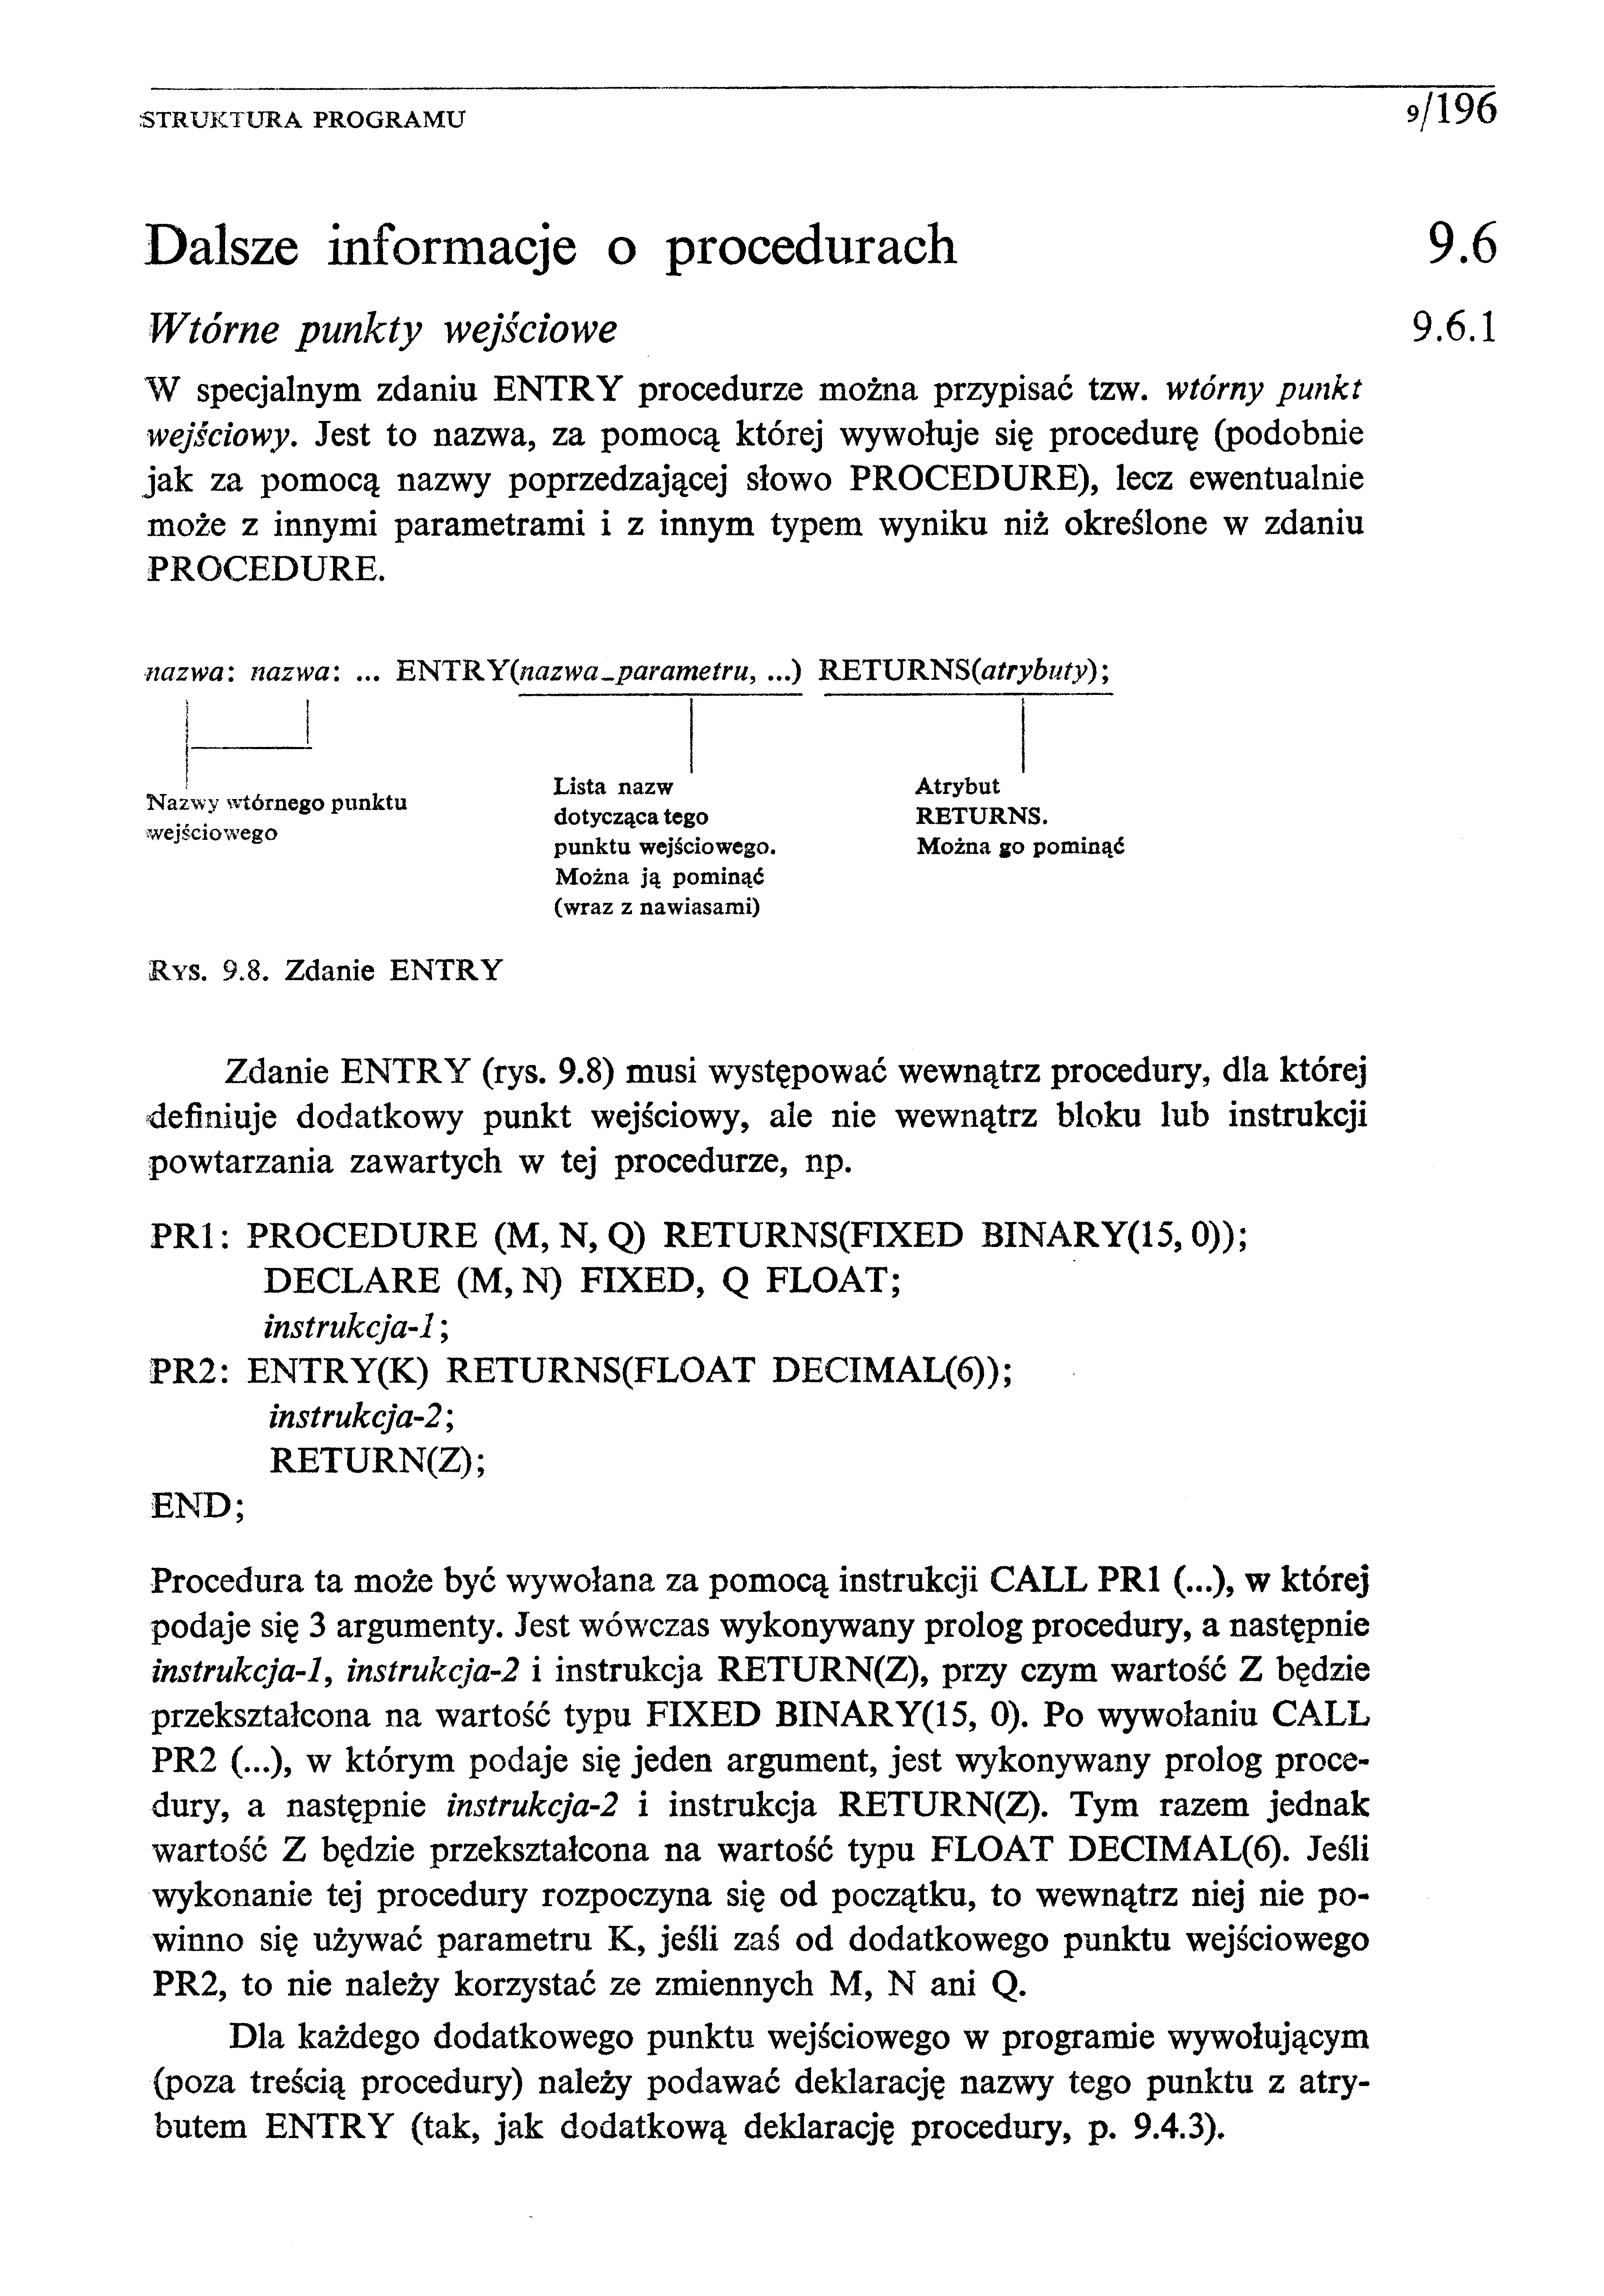
\includegraphics[width=.9\paperwidth]{images/wywod/PLI1_bin.png}}
%     \caption{Widok dekompilacji w programie GHIDRA}
% \end{figure*}
%[]
Przyjrzawszy się zamieszczonemu tam przykładowi, możemy skonstatować, że znamy obecnie znacznie poręczniejszą składnię argumentów domyślnych i należy pozostawić szybko za sobą ten drobny przypis do składni wymarłego języka. Ja wszak nie potrafiłem do końca zapomnieć o tej dziwacznej konstrukcji, nosząc przeświadczenie, że widziałem ją już wcześniej w innym miejscu. Systematyczna kwerenda ujawnia, że podobna składnia ze słowem kluczowym ENTRY pojawia się również w Fortranie\cite[str.~120]{bielecki}, oraz w COBOLU\cite{ibm_manual_on_ENTRY_in_COBOL}. Pewien czas wszakże upłynął, zanim znów przypadkowo dotarłem w miejsce, gdzie owo „entry” zobaczyłem po raz pierwszy -  na liście słów kluczowych C u Kernighana i Ritchiego, opatrzone wyjątkowo lakonicznym opisem, nie ujawniającym powiązanej z nim składni\cite[str.~120]{KiR}
W wydaniu drugim tej książki pojawia się stwierdzenie o wyłączeniu tego słowa kluczowego ze specyfikacji języka\cite[rozdz.~A2.4,~str.192]{KiR2}, odpowiadając już powszechnemu doświadczeniu C, jako języka pozbawionego takiej konstrukcji.

Szerzej zakrojone wysiłki w zakresie archeologii językowej, przedstawiają „ENTRY” i formy podobne, jako dziwaczne skamieliny – występujące powszechnie w pierwszym pokoleniu języków wysokiego poziomu, by potem stopniowo wymrzeć, poprzez zepchnięcie na marginesy standardów, zarzucenie, jak w C, czy zupełne zapomnienie, nie tylko przez programistów, lecz i projektantów języków w czasach późniejszych. W standardach i podręcznikach odbywa się to wymieranie bez obszerniejszych wyjaśnień, a w różnych mniej formalnych tekstach i urywkach, powtarzane są często opinie, jakoby konstrukcja ta miała być (jeszcze w latach 70) przestarzała, niezalecana,  passe, albo wręcz szkodliwa, otoczona aurą, charakteryzującą zazwyczaj rozwiązania wykorzystywane nagminnie w złych praktykach programistycznych. Przytoczę jeden przykład z forum (w odniesieniu do C):

„Really, it isn't a big loss. The concept of one subroutine with multiple entry points was on its way out even before C was new, and it was wise of the standards makers to ignore such a half-baked idea."\cite{delreth_on_entry}

„Naprawdę, to nie jest wielka strata. Koncepcja jednej procedury z wieloma punktami wejścia była w odwrocie jeszcze zanim C stał się nowy, i było mądre ze strony twórców standardów, że zignorowali tak niedopracowany pomysł.” (tłum.)
 
Nawet jeśli komentarze tego typu wygłaszane są przez programistów dość sędziwych, by pamiętać rzeczywiste uzasadnienie rezygnacji z pomysłu, uznają to za fakt dawno dokonany i uzasadniony, niestety nie dzieląc się szerszymi wyjaśnieniami na piśmie, przynajmniej nie dość często, by autor tej pracy je odnalazł. (Chociaż lektura wątku z \cite{delreth_on_entry} rzuca nieco światła na zagadnienie).
Nawet bez uzasadnień z epoki, można łatwo stwierdzić, że owa konstrukcja składniowa jest prostą konsekwencją przeniesienia sposobu pisania procedur wprost z języków niższego poziomu. Wyobraźmy sobie, że programista asemblerowy, w latach 60 napisał procedurę do drukowania zawartości tabeli. Krótka funkcja w C:

%\marginnote{W poniższym listingu: w pierwszym i trzecim for powinno chyba być num cols zamiast num rows}
%Rzeczywiście.
\begin{lstlisting}
void write_table(char *** cells, char ** colnames, int num_cols, int num_rows)
{
    for(int i=0; i<num_cols; i++)
    {
        if(i>0){putchar(',');}
        printf("%s", colnames[i]);
    }
    putchar('\n');
    
    for(int j=0; j<num_rows; j++)
    {
        for(int i=0; i<num_cols; i++)
        {
            if(i>0){putchar(',');}
            printf("%s", cells[j][i]);
        }
        putchar('\n');
    }
}
\end{lstlisting}

Przed językami wysokiego poziomu, byłaby obszerniejsza i mogłaby wyglądać tak:
(w celach demonstracyjnych użyto współczesnego asemblera NASM na architekture IA-32 (x86))

\begin{lstlisting}
write_table:
; Write column names
    xor eax, eax       ; Reset eax for loop variable
    mov ecx, num_cols  ; Number of column names to write
write_colnames:
    cmp eax, ecx       ; Compare current index with num_cols
    jge write_cells    ; If done, jump to write cells

    mov ebx, [colnames + eax * 4] ; Get pointer to current colname
    test eax, eax                 ; If index > 0
    jz .write_name                ; Skip comma on first colname
    mov esi, comma
    call write_string

.write_name:
    mov esi, ebx
    call write_string

    inc eax          ; Increment column index
    jmp write_colnames

write_cells:
    ; Loop through rows
    xor eax, eax      ; Row index
    mov edx, num_rows ; Total rows
row_loop:
    cmp eax, edx
    jge done          ; Exit after all rows are written
    push eax          ; Save row index

    ; Loop through cells in a row
    xor ecx, ecx      ; Reset column index
    mov esi, [cells + eax * 4] ; Get pointer to current row
write_row:
    cmp ecx, num_cols
    jge .next_row     ; Break when all cells in the row are written

    mov edi, [esi + ecx * 4] ; Pointer to cell
    test ecx, ecx
    jz .write_cell    ; Skip comma before first cell
    mov esi, comma
    call write_string

.write_cell:
    mov esi, edi
    call write_string

    inc ecx          ; Increment column index
    jmp write_row

.next_row:
    call write_newline
    pop eax          ; Restore row index
    inc eax
    jmp row_loop
\end{lstlisting}

Wyobraźmy sobie, że ta procedura ta używana jest wielokrotnie w istniejącym oprogramowaniu:
\begin{lstlisting}
...zapisywanie niektórych rejestrów (caller-save registers)
... ustawianie rejerestrów - argumentów
call write_table
...przywracanie rejestrów zapisywanych przez wołającego
\end{lstlisting}
Przypuśćmy, że pewnego dnia księgowy przychodzi do programisty utrzymującego to oprogramowanie i prosi, aby w dwóch z szesnastu przypadków użycia tej procedury, jednak nie drukować nagłówków. Dzisiaj lista parametrów funkcji write\_table zwyczajnie powiększyłaby się o flagę, określającą, czy pisać nagłówek. W asemblerze również można to zwięźle zapisać – dodać na początku procedury
\begin{lstlisting}
jz %rejestr_z_flagą write_cells
\end{lstlisting}
Trzeba jednak wtedy zmienić każde z wywołań procedury, jest to bardziej pracochłonne w języku niskiego poziomu, a jeśli argumenty są przekazywane w rejestrach, nie na stosie (co zdarza się w niektórych architekturach i dzisiaj), to konieczność znalezienia dodatkowego wolnego rejestru miejscu wywołania może zaburzyć ręcznie skonstrowany schemat przydziału rejestrów w okalającej procedurze. (A jak wspomniano, dowiedziono że problem przydziału rejestrów jest NP-zupełny.\cite{REGISTER_ALLOCATION_CHAITIN1981}) Dlatego dość prawdopodobne, że programista zwyczajnie w dwóch miejscach, zamiast
\begin{lstlisting}
call write_table
\end{lstlisting}
napisałby 
\begin{lstlisting}
call write_cells
\end{lstlisting}
write\_table i write\_cells są w istocie jedynie adresami i gdy nie ma rozbudowanego prologu procedury, można ją rozpocząć równie dobrze w innym punkcie w ten sposób. Możemy więc wyobrazić sobie, dlaczego programistom przywykłym do języków niskiego poziomu, taka konstrukcja wydałaby się naturalna:

\marginnote{W poniższym listingu: w pierwszym i trzecim for powinno chyba być num cols zamiast num rows}

\lstset{
    escapechar=|,
    breaklines=true
}
\begin{lstlisting}
void write_table(char *** cells, char ** colnames, int num_cols, int num_rows)
{
    for(int i=0; i<num_cols; i++)
    {
        if(i>0){putchar(',');}
        printf("%s", colnames[i]);
    }
    putchar('\n');
    
    |\textbf{entry}| write_cells(char *** cells, int num_cols, int num_rows);
    for(int j=0; j<num_rows; j++)
    {
        for(int i=0; i<num_cols; i++)
        {
            if(i>0){putchar(',');}
            printf("%s", cells[j][i]);
        }
        putchar('\n');
    }
}
\end{lstlisting}

Nie dziwi też, że takie relikty mogły być zwalczane, gdy próbowano wypracować i rozpowszechnić wśród praktyków, oczywiste dziś pojęcie funkcji, jako bloku kodu robiącego jedną rzecz, z paramtrami wejściowymi oraz wartością zwracaną. Inną konstrukcję bezpośrednio pochodzącą z asemblerów – goto rugowano bardzo długo, ochoczo i niemal z całkowitym sukcesem, podobnie jawne etykiety do niej potrzebne, składniowo skopiowane bezpośrednio z asemblerów. Czy może mieć dla nas ów zabytek paleografii jakiekolwiek znaczenie? Zauważmy, że opisuje on ciekawy byt: funkcja ma z algorytmicznego punktu widzenia jedno wejście i wiele wyjść, on ma zarówno wiele wyjść, jak i wejść.
\begin{figure}[h]
    \centering
    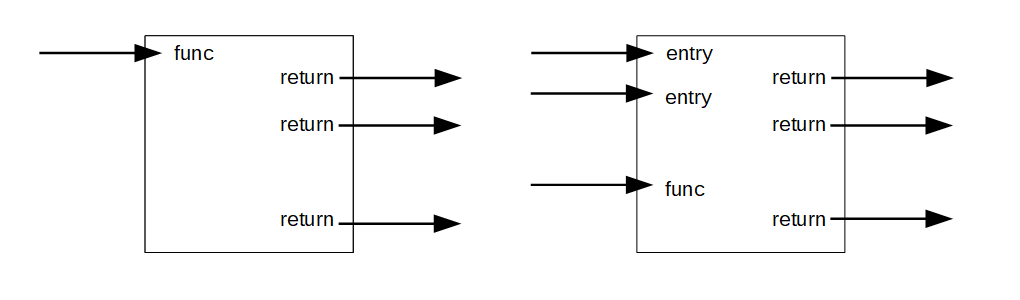
\includegraphics[width=0.6\textwidth]{images/wywod/pudelka.png}
    \caption{Funkcja z jednym punktem wejściowym a procedura z wieloma}
\end{figure}

Wszystkie historyczne implementacje wyróżniają jeden – główny oraz zero lub więcej punktów wejściowych, co zawsze wygląda dość podobnie:

\marginnote{W poniższym listingu: w pierwszym i trzecim dla powinno chyba być liczba kolumn zamiast liczba wierszy}

\lstset{
    escapechar=|,
    breaklines=true
}
\begin{lstlisting}
|\textbf{pisz\_tabelę}|(znak ^^^ krotki,znak ^^ nazwy_kolumn, całk liczba_kolumn, całk liczba_wierszy)
{
    dla(całk i=0; i<liczba_kolumn; i++)
    {
        jeśli(i>0){putchar(',');}
        printf("%s", colnames[i]);
    }
    putchar('\n');
    
    |\textbf{wejście}| pisz_krotki(znak ^^^ krotki, całk liczba_kolumn, całk liczba_wierszy);
    dla(całk j=0; j<liczba_wierszy; j++)
    {
        dla(całk i=0; i<liczba_kolumn s; i++)
        {
            jeśli(i>0){putchar(',');}
            printf("%s", cells[j][i]);
        }
        putchar('\n');
    }
}
\end{lstlisting}
W ramach eksperymentu wznieśmy hasło: „Równe prawa dla wszystkich punktów wejściowych!”, przesuńmy nawiasy,  zamieńmy słowo kluczowe „wejście” na krótszy odpowiednik i otoczmy całą procedurę odpowiednim nagłówkiem:

%\marginnote{W poniższym listingu: w pierwszym i trzecim dla powinno chyba być liczba kolumn zamiast liczba wierszy}
%popr.

\begin{lstlisting}
procedura {
|\textbf{tu}| pisz_tabelę(znak ^^^ krotki,znak ^^ nazwy_kolumn, całk liczba_kolumn, całk liczba_wierszy) -> Nic;
    dla(całk i=0; i<liczba_kolumn; i++)
    {
        jeśli(i>0){putchar(',');}
        printf("%s", colnames[i]);
    }
    putchar('\n');
    
|\textbf{tu}| pisz_krotki(znak ^^^ krotki, całk liczba_kolumn, całk liczba_wierszy)->Nic;
    dla(całk j=0; j<liczba_wierszy; j++)
    {
        dla(całk i=0; i<liczba_kolumn s; i++)
        {
            jeśli(i>0){putchar(',');}
            printf("%s", cells[j][i]);
        }
        putchar('\n');
    }
}
\end{lstlisting}
Uzyskaliśmy w ten sposób dość oryginalną składnię, która nie jest już reliktem asemblerów, lecz organiczną częścią języka. Teraz będzie można eksperymentalnie sprawdzić, czy wielowejściowe procedury są rzeczywiście szkodliwe, lub kłopotliwe w praktyce, czy też da się je kreatywnie wykorzystać. Można rówież powiedzieć, że przypominamy w ten sposób programiście, że nie pracuje z matematycznymi funkcjami, które udają dobrze języki funkcyjne, lecz w prostym, imperatywnym i przede wszystkim proceduralnym języku, nie mającym wielkich ambicji względem abstrakcji matematycznych.

Implementacja tej formy w gramatyce bezkontekstowej jest prosta: nieterminal sygnatury funkcji poprzedzamy słowem kluczowym i traktujemy jak jedną z instrukcji, na równi z np. warunkiem, czy pętlą, (zob. nieterminal instrukcja\_wkroczenia w gramatyce zamieszczonej w \ref{sect:gramatyka}).

\section{System typów}
W poprzednich przykładach niepostrzeżenie pojawiły się nazwy typów. „Typ określa możliwe operacje na bitach oraz uzgodnienia [konwersje] jakie wolno na nich stosować”\cite[str.~259]{waite_goos}. Język wysokiego poziomu nie może obejść się bez spójnego systemu typów, gdyż sprawdzanie ich jest jedną z głównych aspektów analizy semantycznej programu, typy niekiedy sterują też procesem przekładu.

Na system typów składa się zbiór typów podstawowych (atomicznych), zbiór konstruktorów typów, czyli reguł łączenia ich w typy złożone (np. struktur, tablic, czy funkcji – typy „strzałkowe”), oraz określenie operacji na nich dozwolonych, w tym specjalnych unarnych operacji do konwersji pomiędzy typami.
\begin{lstlisting}
całkowite x;
x = y + 7.0;
\end{lstlisting}
Mając pewne użycie operacji $f$, (funkcji, lub operatora), oraz n-elementową krotkę użytych argumentów: $(t_1, t_2, ..., t_n)$, trzeba dysponować mechanizmem określającym, czy dane typy są dozwolone dla tej operacji. W bardziej skomplikowanych przypadkach, gdy istnieje wiele operacji o tej samej nazwie, stanowiących przeładowania nazwy lub operatora, mechanizm kompilatora musi wybrać właściwe dopasowanie argumentów do parametrów formalnych, spróbować dobrać odpowiednie konwersje automatyczne, lub zgłosić zrozumiały błąd.
W powyższym przykładzie, programista spodziewa się, że druga linia zostanie przetłumaczona bez zastrzeżeń, gdyż przywykł do oglądania takich napisów w kontekście matematycznym (fizycznym). Wymaga to wszak zastosowania różnych automatycznych konwersji, w zależności od typu zmiennej y.
\lstset{
    escapechar=|,
    breaklines=true
}
%\marginnote{Proszę wyjaśnić co oznaczają poszczególne poniższe konstrukcje.}
% Jest trochę czytelniej?
\newpage
\begin{center}
\captionof{table}{Możliwe zachowania przy wstawianiu konwersji automatycznych do wyrażenia \lstinline[columns=fixed]{całkowite x = y + 7.0;} w zależności od typu \lstinline{y}.}  \label{tab:title} 
\begin{tabular}{|c|c|}
\hline
%\textbf{Typ y} & \vtop{\hbox{\strut możliwe zachowanie}\hbox{\strut przy wstawianiu konwersji automatycznych}\hbox{\strut do x = y + 7.0;}} \\ \hline
\begin{lstlisting}
całkowite y;
\end{lstlisting}
&
\begin{lstlisting}
x = całkowite(rzeczywiste(y) + 7.0); 
    lub
x = y + całkowite(7.0)
\end{lstlisting}
 \\ \hline

\begin{lstlisting}
rzeczywiste y;
\end{lstlisting}
&
\begin{lstlisting}
x = całkowite(y + 7.0)
\end{lstlisting}
 \\ \hline

\begin{lstlisting}
znak y;
\end{lstlisting}
&
\begin{lstlisting}
analogicznie jak przy całkowitym y, lub błąd
(zależnie od zdefiniowanych konwersji)
\end{lstlisting}
 \\ \hline

\begin{lstlisting}
T y; 
\end{lstlisting}
&
\lstset{
    escapechar=|,
    breaklines=true
}
\begin{lstlisting}
                        błąd 
(chyba, że obsługuje się przeładowanie + dla <T, całk>)
\end{lstlisting}
 \\ \hline

 
%rzeczywista/rzecz           & f64      & double             \\ \hline
\end{tabular}
\end{center}

% \begin{lstlisting}
% całkowite y; => x = całkowita(rzeczywista(y) + 7.0); 
%                     lub
%                 x = y + całkowita(7.0)
                
% rzeczywiste y; => x = całkowita(y + 7.0)

% znak y; => podobnie jak całkowita, lub błąd, 
%         (zależnie od reguł konkretnego języka)

% Typ strukturalny T => błąd
%         (chyba, że zdefiniowano przeładowanie operatora + dla T, całk.)
% \end{lstlisting}

Zagadnienie dobrego zaprojektowania systemu typów, przestaje być proste, gdy włączymy do niego wszystkie powszechnie używane mechanizmy – konwersje jawne i automatyczne, przeładowania nazw i operatorów, polimorfizm oraz typy parametryzowane. W szczególności te ostatnie wydają się tak skomplikowanym konceptem, że często okazują się wykraczać poza wyobrażenia ich twórców\cite{cpp_templates_turing_complete}\cite{taming_wildcards_java}, z pewnością zaś przekraczają możliwości tak małego projektu.
W warunkach tak ograniczonych, na początku rozwoju języka, właściwym pytaniem wydaje się być „Jaki jest najprostszy możliwy w tym wypadku system typów?” Odpowiedź zapewnia system typów maszyny docelowej - LLVM, będący z kolei pierwotnie przystosowany do języków C i C++. Skopiujemy więc w zasadzie system typów C, próbując go wszakże możliwie uprościć.
Typy podstawowe podyktowane są nawet nie przez samo LLVM, lecz przez architektury sprzętu, dysponującego dziś rejestrami całkowitymi o długościach od bajtu do słowa maszynowego (32/64 bity) oraz rozmaitymi rejestrami zmiennoprzecinkowymi, przechowującymi 32 lub 64 bitowe  reprezentacje liczb zmiennoprzecinkowych podług standardu IEEE754. (Pomijamy rejestry wektorowe)
\begin{center}
\begin{tabular}{|c|c|c|}
\hline
\textbf{Projektowany język} & \textbf{LLVM} & \textbf{C/C++} \\ \hline
znak                        & i8       & char               \\ \hline
całkowita/całk              & i64      & long long int      \\ \hline
rzeczywista/rzecz           & f64      & double             \\ \hline
\end{tabular}
\end{center}

Ascetycznie opuszczamy na razie liczby bez znaku, oraz mając okazje tworzyć język od początku, bez wymogów kompatybilności wstecznej, ignorujemy kłopotliwą i niewiele wnoszącą w praktyce dychotomię liczb 32/64bitowych. (LLVM przetłumaczy poprawnie arytmetykę na liczbach 64bitowych również na rozkazy maszyny 32 bitowej, zajmować wszak będzie każda zmienna dwa rejestry, nie będzie to kod efektywny. W roku pisania tej pracy maszyny 32 bitowe są już wyraźną mniejszością)

Nie są to jednak wszystkie typy potrzebne do funkcjonalnego systemu. Konieczne są jeszcze tablice:
\begin{lstlisting}
rzecz^ tabl = nowe [17] rzecz;
\end{lstlisting}
Jako że LLVM posiada wbudowane malloc, kopiujemy składnię alokacji na stercie z C++, przesuwając jedynie liczbę żądanych elementów przed typ.
Do oznaczania wskaźników nie trzeba używać symbolu *. Zapożyczamy semantykę znaku \up\space z niestandardowej implementacji C++ dla .NET (Microsoft C++ CLI). Tam oznaczała ona uchwyt, lub inaczej referencję zarządzaną przez odśmiecacz.(gdyż to .NET i ze zwykłym C++ miał niewiele wspólnego) W projektowanym języku oznaczać będzie jednak \up \space zwykły (nagi wskaźnik), jak w C, lecz należy zaznaczyć, że LLVM oferuje szereg mechanizmów integracyjnych dla odśmiecaczy (garbage collectors) i w dalszym etapie rozwoju projektu można rozważyć użycie, np. odśmiecacza Boehma, jak czyni to język V.\cite{vlang_repo}

Zmiana oznaczenia krotności wskaźnikowej ma jednak przede wszystkim na celu zaznaczenie odmiennej od C semantyki dla prostych referencji do struktur. W C/C++ typy złożone używa się zarówno bezpośrednio (np. zajmując pamięć na stosie)
\begin{lstlisting}
typedef struct A {int b, char c;}A;
<wewnątrz funkcji>
A a;
a.b + (a.c- 'a');
\end{lstlisting}
Lub używa wskaźnika do nich (a w C++ również „referencji”)
\begin{lstlisting}
A* a = new A; albo A* a = malloc(sizeof(A));
a->b + (a->c - 'a');
\end{lstlisting}
Konieczność umieszczenia bardzo podobnego kodu w translatorze dla semantyki struktur „bezpośrednich” i operatora . oraz wskaźników do struktur z operatorem ->, wydaje się w pierwszym podejściu niezachęcające. Obserwujemy też, że wiele języków znakomicie funkcjonuje, używając wyłącznie wskaźników do obiektów, nazywając je referencjami i rezygnując z arytmetyki na nich, np. Java
\begin{lstlisting}
A a = new A(); 
a.b + (a.c- 'a');
\end{lstlisting}
czy Python
\begin{lstlisting}
a = A() 
a.b + (ord(a.c)- ord('a'));
\end{lstlisting}
W odwrotnym kierunku podążył język Go. W nim wskaźniki są konsekwentnie oznaczane przez gwiazdkę, a jeśli jej nie ma, przekazuje się obiekt w całości przez wartość, z wszystkimi tego konsekwencjami.
W żadnym wymienionych języków oprócz C/C++ nie zachowano dychotomii ./->.
Mając na uwadze prostotę translatora, zawsze przekazujmy obiekty typów złożonych przez referencje, używajmy kropki przy dostępie do składowej, a znak \up\space niech oznacza „podniesienie krotności wskaźnikowej” w następujący sposób:

\begin{center}
\begin{tabular}{|c|c|c|c|}
\hline
\textbf{Projektowany język} & \textbf{C} & \textbf{LLVM \tiny{(opaque pointers)}} & \textbf{,,Krotność wskaźnikowa''} \\ \hline
całk        & long long int             & i64 & 0 \\ \hline
całk\up     & long long int *           & ptr & 1 \\ \hline
całk\up     & long long int <nazwa>[]   & ptr & 1 \\ \hline
całk\up\up  & long long int **          & ptr & 2 \\ \hline
-           & T                         & T   & 0 \\ \hline
T           & T*                        & ptr & 1 \\ \hline
-           & T <nazwa> []              & ptr & 1 \\ \hline
T\up        & T**                       & ptr & 2 \\ \hline
T\up\up     & T***                      & ptr & 3 \\ \hline
\end{tabular}
\end{center}

Widzimy też, że można wyzbyć się chwilowo tablic o znanej wielkości, używając w ich miejsce wskaźników. W C int *t  nie jest równoważne, int t[] a już na pewno nie int t[20],w sensie ścisłej równości typów, dwa ostatnie zachowują się jednak, jakby były podtypem pierwszego (zwie się to rozpadem tablic do wskaźników - „array to pointer decay”). Zważywszy na to, że tak jak C nie jesteśmy zapewnić zadowalającego dla dzisiejszych zastosowań sprawdzania granic tablic, uproszczenie pozwalające indeksować dowolny wskaźnik wydaje się być akceptowalne – do tablic wystarczą typy wskaźnikowe.
\begin{lstlisting}
całk ^ t; ... całk i = t[3];
\end{lstlisting}

Struktury niech otrzymają możliwie prostą składnię:
\begin{lstlisting}
typ Zespolona {rzecz rz; rzecz ur;};
\end{lstlisting}
Definiujmy w ten sposób jedynie tablice wskaźników, lecz nie samych obiektów:
\begin{center}
\begin{tabular}{|c|c|}
\hline
\textbf{Projektowany język} &  \textbf{C} \\ \hline
Zesp z; z[1] - niedozwolone & Zesp * z; z[1] – dozwolone – tablica struktur \\ \hline
Zesp\up \space z; z[1] – dozwolone – tablica wskaźników & Zesp * z[]; z[1] – dozwolone – tablica wskaźników \\ \hline
\end{tabular}
\end{center}

Takie poświęcenie oznacza kilka procedur w translatorze mniej… nie wydaje się również, żeby programista, który już zacznie myśleć w kategoriach bardziej współczesnych referencji (takich jak w Javie), przypominał sobie zbyt często o tablicach struktur rozmieszonych jednorodnie w pamięci.

Pozostaje jeszcze do rozstrzygnięcia kwestia pustych referencji. Powszechnie wskazuje się na nie, jako na przyczynę różnych problemów, błędów i podatności. Niestety do ich skutecznego, lecz jednocześnie znośnego dla programisty wyeliminowania, potrzebny jest o wiele potężniejszy system typów i mechanizm zarządzania pamięcią – ,,garbage collector'' lub ,,borrow checker''. Zmuszeni jesteśmy zatem zaakceptować napisy podobne do poniższego:
\begin{lstlisting}
T t = pusty;    
\end{lstlisting}
 gdzie „pusty” odpowiada wyróżnionej wartości oznaczającej nie wskazywanie na żaden obiekt. Powstaje  pytanie, jakiego typu powinien być ten specjalny literał. Dość powszechnie wiadomo, że w języku C pierwotnie makro NULL rozwijane było do 0.\cite[str.~214]{KiR} To dość naturalne, w kontekście wczesnego C, jeszcze przed standardem ANSI. System typów był wtedy mniej ścisły, w wielu miejscach można było je opuszczać, a kompilator domyślnie zakładał typ całkowity, w dodatku używając go automatycznie również jako typu wskaźnikowego. Krytykę tak swobodnego podejścia, rozmontowującego w praktyce kontrolę typów można znaleźć w pierwszym wydaniu podręcznika Kernighana i Ritchiego(\cite{KiR}). Gdy jednak wprowadzono  typy void * do C, rozsądniejszą wartością dla NULL stało się ((void*)0), co przynajmniej wyeliminowało niejawne rzutowania z typu całkowitego na wskaźnikowe, lecz dalej nie jest to stan satysfakcjonujący:
\begin{lstlisting}
(wyrażenie) T* t = NULL;
(typy)         T*  void*
\end{lstlisting}
T* jest podtypem void*, lecz nie odwrotnie, ściśle rzecz ujmując jest to podstawienie niedozwolone, tak jakby w Javie napisać np.
\begin{lstlisting}
OutputStream s = (Object)obj;
\end{lstlisting}
lub ogólniej:
\begin{lstlisting}
class A extends B[...] B b; A a = b;
\end{lstlisting}
Nie można zezwalać na niejawną konwersję z void* do dowolnego typu, niweczy to efektywność statycznego typowania, które ma zagwarantować, że nie da się wykonać operacji na obiekcie niewłaściwego typu. Rozwiązaniem stosowanym w C++, choć znanym już dużo wcześniej\cite[str.256 - zob. nil\_typ]{waite_goos}, jest wprowadzenie specjalnego, osobnego typu, którego jedynym okazem jest literał pustej referencji, a następnie zdefiniowanie domyślnej konwersji od niego do dowolnego konkretnego typu referencyjnego (lecz nie do void*). W ten sposób możemy zachować jedynie jawne konwersje do i z nieokreślonego typu referencyjnego,  zachowując funkcjonalność pustego literału. W C++ ten typ nazwano nulptr\_t, w programie rozwijanego translatora nosi nazwę TpPustego i podobnie jak w C++, użytkownik nie musi być świadom jego istnienia.
(Ze względu na kompatybilność wsteczną, w C++ nie zmieniano definicji makra NULL, lecz dodano nowy literał nullptr, mający go zastępować)
\begin{center}
\begin{tabular}{|c|c|}
\hline
\textbf{Projektowany język} & \textbf{C++} \\ \hline
\begin{lstlisting}
(wyrażenie) T t = pusty;
(typy)       T    TpPustego^
\end{lstlisting}
& 
\begin{lstlisting}
(wyrażenie) T * t = nulptr;
(typy)         T*   nulptr_t
\end{lstlisting} \\\hline
\end{tabular}
\end{center}
% \begin{lstlisting}
% (wyrażenie) T t = pusty;
% (typy)       T  = TpPustego^
% T * t = nulptr;
% T* = nulptr_t
% \end{lstlisting}

Możemy więc podać cały diagram konwersji w tworzonym języku:

\begin{figure}[h]
    \centering
    \includesvg[width=0.6\textwidth]{images/3.konwersje.svg}
    \caption{Diagram konwersji w projektowanym języku}
\end{figure}

Przyjąłem zasadę, żeby nie definiować konwersji automatycznych, które są jednocześnie zwężające (prowadzą do utraty informacji), ponieważ może to niekiedy konfundować użytkownika, a nawet prowadzić do podatności bezpieczeństwa\cite[str.~260]{Reversing}.

\section{Gramatyka języka}
\label{sect:gramatyka}
Język programowania można dość dokładnie opisać w formie dobrze znanej w matematyce definicji rekurencyjnej, jak czyni to wstępny opis ALGOLA\cite{ALGOL_PRELIMINARY_REPORT} czy SAKO\cite{SAKO}. Aby skonstruować parser dla danego języka, potrzebny jest wszak ścisły opis i w roli tej znakomicie sprawdza się gramatyka bezkontekstowa.

Wyjaśniwszy co istotniejsze decyzje podjęte przy projektowaniu języka, można w tym miejscu zamieścić jego gramatykę w całej rozciągłości.
Zostanie ona przedstawiona w postaci nieznacznie różniącej się od klasycznej rozszerzonej notacji Backusa-Naura (EBNF), a będącej rzeczywistym plikiem źródłowym dla generatora parserów wykorzystywanym w projekcie. Ma to na celu zademonstrowanie użyteczności takich gramatyk nie tylko jako specyfikacji konstrukcji parsera, lecz jako zwartej, czytelnej dla człowieka i przede wszystkim ścisłej definicji składni języka.

%\marginnote{Poniższa gramatyka wychodzi poza marginesy strony}
%Już powinno byc lepiej. 
\newgeometry{left=2.4cm,right=2.4cm,top=2cm,bottom=2cm} % Set thinner margins
\lstset{
    escapechar=@,
    breaklines=true
}
\begin{lstlisting}[basicstyle=\scriptsize\ttfamily,breaklines=true]
grammar plpl;
program : (byt_globalny)* EOF;
byt_globalny: procedura | deklaracja_typu | deklaracja_nazwy;
deklaracja_typu: deklaracja_aliasu_typu | deklaracja_typu_strukturalnego;
deklaracja_aliasu_typu:'typ'  nowa_nazwa_typu 'jak' NAZWA_TYPU ';';
deklaracja_typu_strukturalnego   : 'typ'  nowa_nazwa_typu  '{' ( deklaracja_nazwy )* '}' ';';
nowa_nazwa_typu:  NAZWA | NAZWA_TYPU; //użytkownik wprowadza nowy typ


procedura   :  PROCEDURA '{' lista_instrukcji  '}';
lista_instrukcji   : instrukcja+;
instrukcja   :   instrukcja_wyboru
             |   instrukcja_petli
             |   instrukcja_przerwania_petli
             |   instrukcja_kontynuacji_petli
             |   instrukcja_wkroczenia
             |   instrukcja_powrotu
             |   instrukcja_zlozona
             |   instrukcja_prosta
             |   instrukcja_pusta
             |   deklaracja_nazwy;


instrukcja_wyboru   : ('jeśli'|'jesli'|'gdy') '(' wyrazenie ')' instrukcja  ('inaczej'  instrukcja)?;
instrukcja_petli   : 'dopóki' '(' wyrazenie ')' instrukcja;
instrukcja_powrotu   : 'zwróć' wyrazenie? ';';
instrukcja_wkroczenia   : ('zacznij'| 'tu')  NAZWA '(' lista_parametrow_formalnych ')' ('->' obutyp)? instrukcja;
instrukcja_przerwania_petli   : PRZERWIJ ';';
instrukcja_kontynuacji_petli   : KONTYNUUJ ';';
instrukcja_zlozona  : '{'  lista_instrukcji?  '}';
instrukcja_prosta  :   wyrazenie ';';
instrukcja_pusta   : ';';

lista_parametrow_formalnych : (deklaracja_parametru  (',' deklaracja_parametru)* (',' ELIPSA )? )?;
deklaracja_parametru   : deklarator_bez_przypisania przydomkowany_prawotyp| przydomkowany_lewotyp  deklarator_bez_przypisania;
@\newpage@

wyrazenie :
        wyrazenie '(' lista_parametrow_aktualnych ')'               #wyrazenieWywolanie
      | lewotyp '(' lista_parametrow_aktualnych ')'                 #wyrazenieKonwersja
      | alokacja                                                    #wyrazenieAlokacja
      | dealokacja                                                  #wyrazenieDealokacja
      | wyrazenie '['  wyrazenie  ']'                               #wyrazenieSelekcjaTablicowa
      | wyrazenie '.' NAZWA                                         #wyrazenieSelekcjiSkladowej
      | adr='&' wyrazenie                                           #wyrazenieAdres
      | neg='!' wyrazenie                                           #wyrazenieNegacja
      | znak=('-'|'+') wyrazenie                                    #wyrazenieZnak
      | <assoc=right> wyrazenie '^' wyrazenie                       #wyrazeniePoteg
      | wyrazenie mult=('*'|'/'|'%') wyrazenie                      #wyrazenieMult
      | wyrazenie addyt=('+'|'-') wyrazenie                         #wyrazenieAddyt
      | wyrazenie porownanie=('=='|'!='|'>'|'<'|'<='|'>=')wyrazenie #wyrazeniePorownanie
      | wyrazenie logicz=('&&'|'||')wyrazenie                       #wyrazenieLogicz
      | <assoc=right> wyrazenie '=' wyrazenie                       #wyrazeniePrzypisanieZwykle
      | <assoc=right> wyrazenie '^=' wyrazenie                      #wyrazeniePrzypisaniePoteg
      | <assoc=right> wyrazenie mult=('*='|'/='|'%=') wyrazenie     #wyrazeniePrzypisanieMult
      | <assoc=right> wyrazenie addyt=('+='|'-=') wyrazenie         #wyrazeniePrzypisanieAddyt
      | NAZWA                                                       #wyrazenieNazwa
      | literal                                                     #wyrazenieLiteral
      | '(' wyrazenie ')'                                           #wyrazenieNawiasy
      ;

alokacja: NOWY wielkosc_alokowanej_tablicy? obutyp;// buf = nowy [128] całk; vs buf = new int[128]; - przestawiony rozmiar przed typ względem C++
wielkosc_alokowanej_tablicy: '[' wyrazenie ']';
dealokacja:ZAPOMNIJ '('wyrazenie')';

lista_parametrow_aktualnych : (wyrazenie  (',' wyrazenie)*)?;

deklaracja_nazwy   :
     deklarator_bez_przypisania prawotyp /*('='wyrazenie)?*/ ';'
     | przydomkowany_lewotyp (deklarator_bez_przypisania|deklarator_zlozony_z_przypisaniem) (',' (deklarator_bez_przypisania|deklarator_zlozony_z_przypisaniem))*  ';';

deklarator_bez_przypisania : NAZWA;
deklarator_zlozony_z_przypisaniem : NAZWA  '='  wyrazenie;

przydomkowany_lewotyp: przydomki lewotyp;
przydomkowany_prawotyp: przydomki prawotyp;
przydomki : (STATYCZN|AUTOMATYCZN|STAL)*;

lewotyp : nazwa_typu (podnosnik_krotnosci_wskaznikowej)*;
prawotyp : (podnosnik_krotnosci_wskaznikowej)* typ_strzalkowy;
obutyp: lewotyp | prawotyp;
podnosnik_krotnosci_wskaznikowej: '^';

typ_strzalkowy: '(' lista_parametrow_strzalkowego ')' '->' obutyp;
lista_parametrow_strzalkowego : (parametr_strzalkowego  (',' parametr_strzalkowego)* (',' ELIPSA )?)?;
parametr_strzalkowego: obutyp;

nazwa_typu:  NAZWA_TYPU | TCALK | TRZECZYW  | TZNAK | TNIC;

literal: literal_atomiczny | literal_tablicowy;
 literal_atomiczny   :  CALK  |  ZMIENN  |  ZNAK_DOSL ;
 literal_tablicowy   : NAPIS_DOSL | PUST;
@\newpage@
// LEKSER

 ELIPSA:'...';
 TNIC : 'Nic';
 TCALK: 'ca'[\u0142]'k'('owit'([yea]|'ych')?)?;
 TRZECZYW: 'rzecz'('yw'('ist'[yea])?)?;
 TZNAK: 'znak';

 PUST: 'pust'[yea];

 STATYCZN: 'statyczn'[yea];
 AUTOMATYCZN : 'automatyczn'[yea];
 STAL : 'sta'[\u0142][yea];

 PROCEDURA: 'proc'| 'procedura';
 NOWY: 'now'[yea];
 ZAPOMNIJ: 'zapomnij';

 PRZERWIJ : 'przerwij';
 KONTYNUUJ:'kontynuuj';

 ZMIENN :  CALK'.'CALK; //zmiennoprzecinkowa liczba
 CALK :   [0-9]+ ;   //zwykła liczba
 ZNAK_DOSL
     :   '\'' ( EscapeSequence | ~('\''|'\\') ) '\''
     ;

 NAPIS_DOSL
     :  '"' ( EscapeSequence | ~('\\'|'"') )* '"'
     ;

 fragment
 EscapeSequence
     :   '\\' ('b'|'t'|'n'|'f'|'r'|'\''|'\\');
//RZECZYWISTE TOKENY, ZAMIENIANE PRZEZ PREPROCESOR
     NAZWA:[\u9670];
     NAZWA_TYPU:[\u967D];
     ID : ([A-Za-z_]|OGONEK)([0-9A-Za-z_]|OGONEK)*;//zob.preprocesor
//TOKENY DZIAŁAJĄCE BEZ PREPROCESORA
//    NAZWA_TYPU :  ([A-Z]|WIELKI_OGONEK)([0-9A-Za-z_]|OGONEK)*;//zaczyna się z dużej litery
//    NAZWA : ([a-z_]|OGONEK)([0-9A-Za-z_]|OGONEK)*;//zaczyna sie z małej litery
//    ID:'$';

//polskie ogonki
 fragment OGONEK : [\u0104\u0105\u0106\u0107\u0118\u0119\u0141-\u0144\u015A\u015B\u0179-\u017C\u00D3\u00F3];
 fragment WIELKI_OGONEK: [\u0104\u0106\u0118\u0141\u0143\u015A\u0179\u017B\u00D3];
 //104,105 - Ąą
 //106,107 - Ćć
 //118,119 - Ęę
 //141,142 - Łł
 //143,144 - Ńń
 //15A,15B - Śś
 //179,17A - Źź
 //17B,17C - Żż
 //D3,F3   - Óó


 LINE_COMMENT : '//' .*? (EOF|'\r'? '\n') -> skip ;
 COMMENT : '/*' .*? '*/' -> skip ;
 WS  :   [ \t\r\n]+ -> skip ; // ignorowanie białych znaków
\end{lstlisting}
\lstset{
    escapechar=|,
    breaklines=true
}
\restoregeometry % Restore the original page margins after the listing

Aby uczynić zadość przyjmowanej szeroko definicji gramatyki bezkontekstowej\cite[str.~158]{hopcroft_automaty}, musimy podać, że zbiorem symboli nieterminalnych są te, zapisywane małymi literami w produkcjach, zbiorem terminali te pisane wielkimi (wedle konwencji generatorów parserów, nie podręczników lingwistyki formalnej, a przynajmniej \cite{hopcroft_automaty}), zaś symbolem startowym (początkowym) jest „program”. 

Jest to język bezkontekstowy, o ile za symbole terminalne przyjmujemy tokeny, gdyż każda produkcja gramatyki ma tylko jeden nieterminal po lewej stronie. Jeśli zaś rozpatrujemy ten język jako ciąg znaków, nie tokenów, wykracza on poza tę klasę, ze względu na kontekstowość mechanizmu odróżniającego tokeny NAZWĄ i NAZWA\_TYPU.

W zaimplementowanym translatorze istnieje komponent umieszczony pomiędzy lekserem a parserem, działający na strumieniu tokenów i przekształcający tokeny ID według następującego automatu:

\begin{figure}[h]
    \centering
    \includesvg[width=0.6\textwidth]{images/wstep/preprocesor.svg}
    \caption{Automat odpowiadający nieterminalowi deklaracja\_typu, zbierający wpierw nazwy wszystkich nowych typów. ($\Sigma$ : zbiór terminali) }
\end{figure}
Uzyskawszy w ten sposób zbiór nazw wszystkich typów użytkownika wprowadzonych w jednostce translacji (a można je deklarować jedynie globalnie, ze względu na umiejscowienie symbolu deklaracja\_typu), przekształca się każdy token ID albo na token NAZWA\_TYPU, jeśli jego tekst należy do zbioru nazw typów, albo NAZWA w przeciwnym wypadku.

Popularne języki, takie jak C nie są w rzeczywistości zupełnie bezkontekstowe, a mądre wyznaczenie granic pomiędzy lekserem (z językiem regularnym), parserem (bezkontekstowym), a semantyką (pisaną w języku kompletnym w sensie Turinga), tak aby optymalnie wykorzystać możliwości każdego z tych mechanizmów, jest istotnym zadaniem w projektowaniu translatora.\cite{DRAGON_BOOK}

Uważny czytelnik może zwrócić też uwagę na drobne niedopatrzenie w tym rozdziale – zapomniano  przetłumaczyć projekt języka na angielski. To odstępstwo od zwyczaju będzie wymagało szerszych wyjaśnień.

\section{Dlaczego po polsku?}
%1. Od dawna nikt nie próbował
Pierwszym uzasadnieniem dla próby skonstruowania języka programowania „po polsku”, jest to , że obecnie żaden taki język nie istnieje \marginnote{Rozumiem, że chodzi o język ogólnego zastosowania?}. Każdy, kto przeprowadził kwerendę w tym zakresie, zorientuje się szybko, że publicznie wiadomo o dokładnie jednej próbie stworzenia języka ogólnego przeznaczenia z polskim substratem.%?? - czy o to, że są domenowe po polsku, czy o to, że ma byc ogólnego zastosowania, nie przeznaczenia

W latach 60 w Zakładzie Aparatów Matematycznych Polskiej Akademii nauk, dla serii rodzimych komputerów (choć inspirowanych IBM 701), stworzono System Automatycznego Kodowania, nazywany częściej językiem SAKO.\cite{SAKO} Było to niewątpliwie ciekawe przedsięwzięcie, jako jedyne w historii proponujące odpowiedź na główną przeszkodę w pisaniu programów „po polsku” - konieczność pomijania odmiany wyrazów w naszym języku. W SAKO zaproponowano proste, lecz akceptowalne wtedy rozwiązanie – identyfikowanie symbolu tylko na podstawie kilku pierwszych jego liter (co pozwala na różne końcówki). Wobec liczonego w ledwie tysiącach słów maszynowych rozmiaru pamięci tych komputerów i konsekwentnie rozmiarów pisanych programów, nie stanowiło to praktycznego problemu.
Niektóre aspekty tego języka są niezwykle interesujące, czego dobrym przykładem jest obsługa przepełnień, do czego przeznaczono specjalną instrukcję:
\begin{lstlisting}
BYL NADMIAR , np.:
GDY BYL NADMIAR: 1A, INACZEJ 3 
\end{lstlisting}
To z pewnością więcej, niż współczesny mu FORTRAN, czy C, które „rozprawiają się” z problemem, orzekając w swych standardach, że powoduje on zawsze niezdefiniowane zachowanie (undefined behaviour) i przenosząc całą odpowiedzialność na programistę.

Wymarł jednak ten język, wraz z komputerami zawierającymi rodzimą myśl techniczną i od tego momentu programuje się wyłącznie po angielsku.
Poszukując innych przykładów, nie znajdziemy praktycznie nic, prócz wąskich języków domenowych. Istniała polska wersja programu MS Logo (Logomaoja), gdzie przetłumaczono rozkazy podawane figuratywnemu żółwiowi na język polski, a jako, że zawierał on również instrukcj warunkowe, pętle i możliwość definiowania zmiennych, to przyznać mu należy cechę kompletności Turinga. Można cierpko stwierdzić, że oprócz kilku narzędzi edukacyjnych, okazjonalnie uzyskujących polskie tłumaczenia, jedynym językiem (w dodatku czysto funkcyjnym) opartym polskim substracie, posiadających setki tysięcy, a może miliony użytkowników w naszym kraju są... formuły Excela.

Używanie jedynie czterech (czasem trzech) pierwszych liter symbolu do jego identyfikacji, byłoby przy dzisiejszej objętości programów niepraktyczne. Niniejsza praca nie podejmie wszak postawionego przez SAKO pytania o właściwą formę języka programowania „po polsku”, lub opartego na języku fleksyjnym w ogóle (nie aglutynacyjnym, jak angielski) – wykracza to poza jej zakres, którego domknięciem w najlepszym wypadku będzie skonstruowanie translatora posiadającego techniczne możliwości obsługi języka tego rodzaju, na razie ograniczając wszak inwencje składniową do minimum, w pragmatycznym celu zapewnienia w pierwszej kolejności niezawodności i odpowiedniej architektonicznej bazy, korzystając z której można by język ów rozbudować.

%2. Polskie dziedziny problemów
Choć zdarzają się przypadki niemal religijnego przywiązania do jednego języka, większość programistów doskonale zdaje sobie sprawę, że do różnych problemów, najodpowiedniejsze są różne języki. Istnieją też problemy, które opisywane są całkowicie, lub prawie całkowicie po polsku. Spójrzmy na przykład xml-a będącego fragmentem UPO JPK VAT (urzędowego potwierdzenia odbioru jednolitego pliku kontrolnego VAT).
\begin{lstlisting}
<Potwierdzenie wersjaSchemy="7.0">
            <NazwaPodmiotuPrzyjmujacego>Ministerstwo Finansów</NazwaPodmiotuPrzyjmujacego>
            <NumerReferencyjny>bbde363301605dcc000000aa010cf2c1</NumerReferencyjny>
            <SkrotDokumentu>[Dv4LGHivk8XrCaUTc2aekUfHpBd6kmNMFEDmKMdnHls=]</SkrotDokumentu>
            <SkrotZlozonejStruktury>fce472fdc724ee911196b9ea7c21bc81</SkrotZlozonejStruktury>
            <NazwaStrukturyLogicznej>Schemat_JPK_V7K(2)_v1-0E.xsd</NazwaStrukturyLogicznej>
            <DataWplyniecia>2024-12-12T18:15:22.5316007+01:00</DataWplyniecia>
            <CelZlozenia>1</CelZlozenia>
            <RokCE>2024</RokCE>
            <MiesiacCE>11</MiesiacCE>
            <StempelCzasu>MjAyNC0xMi0xMlQxODoxNToyMi41MzE2MDA3KzAxOjAw</StempelCzasu>
            <NIP1>6781607420</NIP1>
            <KodUrzedu>1209</KodUrzedu>
            <KodFormularza>JPK_V7K (2)</KodFormularza>
            <Przyjeto>true</Przyjeto>
</Potwierdzenie>
\end{lstlisting}
W tym pojedynczym przykładzie odbijają się zarówno zalety zastosowania rodzimego języka do opisu rodzimej rzeczywistości, jak i egzemplifikują przypadki mieszania polskiego z angielskim, które dla niektórych argument wystarczający na rzecz całkowitego zaniechania prób użytkowania polszczyzny w informatyce. Trudno się dziwić, różnorakie ,,wersjeSchemy'', czy ,,Przyjęto - true'' są szpetnymi zrostami, z którymi niejednokrotnie miewamy do czynienia. Jeśli chce się wykorzystywać określony substrat językowy, trzeba czynić to konsekwentnie przynajmniej wewnątrz lokalnych struktur składniowych.

Kolejnym oczywistym przypadkiem polskich dziedzin problemów są reguły podatkowe, których mnogość w tym kraju jest nam wszystkim dobrze znana i zapewnia chociażby stałą niszę rynkową dla miejscowego oprogramowania ERP dla biznesu, gdyż produkty zachodnie ich nie uwzględniają.

Nie musimy wszakże odwoływać się do przykładów zależnych tak silnie od arbitralnych uwarunkowań. Czasem dziedzina problemu naturalnie nie zawiera języka angielskiego. 

Usłyszałem kiedyś następujące pytanie: „Cykl czytań mszalnych liczy cztery lata, czy podczas tego okresu odczytuje się cały tekst Biblii?”. Dysponując tekstem oraz siglami czytań na każdy dzień, o co nietrudno, da się to sprawdzić, pisząc prosty skrypt. Można przypuszczać, że gdyby napisano go w Pythonie mógłby zawierać fragment podobny do zamieszczonego poniżej:
\begin{lstlisting}
for day, siglum in cycle:
	for verse in split_verses(siglum):
		verses[verse] |= {day}    
\end{lstlisting}

Obiekty dziedziny problemu noszą w istocie polskie nazwy i czy dodawaniem do ich zbioru języka angielskiego nie jest „mnożeniem bytów ponad potrzebę?”
\begin{lstlisting}
dla dnia, siglum spośród cyklu:
	dla wersu spośród wydzielonych_wersów(z: siglum):
		wersy[wers] |= {dzień}
\end{lstlisting}
Sama konieczność używania języka angielskiego, nie stanowi już chyba dla nikogo związanego z branżą większego problemu, niesie jednak ze sobą ukryte koszty, ilekroć stosujemy go do opisu rodzimych problemów. Moje doświadczenie zawodowe zawiera pracę nad systemem, który choć występuje w wersji angielskiej w aplikacjach mobilnych, to działa wyłącznie na terytorium Polski i posługuje się polską nomenklaturą w dziedzinie bytów i procesów biznesowych, we wszystkich miejscach – od panelu przeglądarkowego używanego przez operatorów, przez dokumentację aż do nieoficjalnych rozmów – wszędzie, prócz samego kodu. Przetłumaczenie podstawowych nazw encji, rzecz jasna nie pochłonęło wiele wysiłku, poziom trudności wzrósł na przykład dla nazewnictwa księgowego. Zapewne nie istnieje dokładny semantyczny odpowiednik nazw dokumentów KP/KW (kasa przyjęła, wydała) w języku angielskim, jak i wielu innych, zwłaszcza jeśli odnoszą się do systemu prawnego. Inna natura prawa anglosaskiego względem systemów kodeksowych, do których nasz należy, powoduje, że odpowiedniość pewnych terminów może być nawet złudna. Równie wiele czasu zaprzepaścić można szukając rozsądnego tłumaczenia neologizmu będącego dziełem działu marketingowego, choć działającym zupełnie realnie i potrzebującego osobnej encji w bazie danych i kodzie serwerowym. W takim wypdaku dychotomia nomenklatury jawi się jako skryty, lecz stale obecny koszt, 

Przypuszczam również, że mogą istnieć jednostki niekiedy znużone nieustanną wszechobecnością angielszczyzny w pracy informatyka, które z chęcią, dla odmiany napisałyby niewielki skrypt, bądź fragment aplikacji po polsku, lub zwyczajnie zaciekawione by były, jak taki język „wyglądał” i jak sprawowałby się w praktyce.


	\chapter{Implementcja translatora}
\section{Parser}
Istnieje ścisła zależność pomiędzy każdym typem języków w hierarchii Chomskiego, ich gramatykami i automatami rozpoznającymi napisy w tych językach.\cite{CHOMSKY1959}\cite{hopcroft_automaty}
\begin{center}
\begin{tabular}{|c|c|c|}
\hline
\textbf{Stopień w hierarchii} & \textbf{Gramatyka} & \textbf{Automat} \\ \hline
0 & Struktur frazowych (nieograniczona) & Maszyna Turinga \\ \hline
1 & Kontekstowa & Liniowo ograniczony\\ \hline
2 & Bezkontekstowa & Ze stosem\\ \hline
3 & Regularna & Skończenie stanowy\\ \hline
\end{tabular}
\end{center}

Dla automatycznej analizy składniowej są użyteczne zazwyczaj dwa dolne stopnie tej hierarchii. Analizę leksykalną przeprowadza się definiując tokeny z użyciem języków regularnych, (Chociaż napisanie efektywnego leksera jest daleko trudniejsze niż użycie biblioteki do tzw. ,,regexów'', zob. osiemdziesięciostronicowy rozdział trzeci w podręczniku\cite{DRAGON_BOOK}).

Samo egzystencjalne twierdzenie o istnieniu automatu ze stosem rozpoznającego język bezkontekstowy, niewielką jest pociechą dla piszącego jego translator – potrzebny jest konkretny sposób jego konstrukcji. Nie jest to zagadnienie trywialne i poświęcono mu wiele uwagi w pierwszych dekadach rozwoju języków wysokopoziomowych. W tekście tego rodzaju, nie jest możliwe choćby naszkicowanie kształtów wielkiego gmachu lingwistyki formalnej, ani nawet teorii parsingu. Powiedziane zostanie zaledwie tyle, by umotywować wybór narzędzia do analizy składniowej.

Istnieje kilka algorytmów konstrukcji automatu dokonującego rozbioru zdań w języku opisywanym zadaną gramatyką bezkontekstową. Automat taki nazywany bywa również parserem i miano ta odpowiada jego naturze – bo istotnie wydziela części (łac. - pars) zdania, konstruując drzewo składniowe, gdzie liśćmi są terminale, gałęziami symbole nieterminalne, a korzeniem symbol startowy (choć w praktyce najłatwiej stworzyć parser jedynie rozpoznajacy, czy dany napis należy do języka, czy nie, samo zachowanie parsera zawiera informację o strukturze składniowej zdania, lecz aby ją wydobyć i skonstruować drzewo, potrzebna jest dodatkowa praca)\cite{DRAGON_BOOK}.
%[rysunek dodać przykładowy]

Najprościej wyjaśnić można działanie parsera rekursywnie zstępującego (recursive descent). Konstrukcja jego jest w zasadzie trywialna. Załóżmy, że mamy produkcje gramatyki:

\begin{lstlisting}[numbers=left]
instr: 'jeśli' wyr 'to' instr 'koniec';
instr: 'dopóki' wyr 'to' instr 'koniec';
instr: lista_instr;
lista_instr: instr ';' lista_istr;
lista_instr: |$\epsilon$|; (pusta prawa strona produkcji)
\end{lstlisting}

Wystarczy, że zaopatrzymy się w analizator leksykalny z funkcją nast(), która zwraca następny token, dopasuj(t), która konsumuje token t ze strumienia wejściowego, to możemy niemal wprost „przepisać” gramatykę na procedury parsera: (zaadaptowane z \cite[str.~70]{DRAGON_BOOK})

\begin{lstlisting}
void instr(){
	switch(nast())
	case 'jeśli': wyr(); dopasuj('to'); instr(); dopasuj('koniec'); break; 
            (zob. produkcję (1))
	case 'dopóki': wyr() dopasuj('to'); instr(); dopasuj('koniec'); break;
            (zob. produkcję (2))
	default : zgłoś("Błąd składnoiwy")
}
\end{lstlisting}
Dopasowujemy terminale, a dla nieterminali generujemy podprocedury odpowiadające produkcjom mającym dany symbol po lewej stronie.
Nie skonstruujemy wszak w ten sposób parsera wyrażeń arytmetycznych:
\lstset{escapechar=@,}
\begin{lstlisting}
Gramatyka: 
wyr: wyr * wyr| wyr + wyr;

Procedura parsera: 
void wyr()
{
    wyr(); '+' wyr()...
}
\end{lstlisting}
\lstset{escapechar=|,}
gdyż oznaczałoby to nieskończoną rekursję. (Rekursja lewostronna jest ogólnie zakazana dla parserów zstępujących, jeśli nie usunie się je przekształcając gramatykę.)

Podobnie działa tabelaryczny parser LL, z tą różnicą, że ma formę jawnego automatu ze stosem, a nie zbioru procedur. Istnieją różne odmiany algorytmu generacji zbioru stanów takich parserów – kanoniczne LL(k) są w stanie rozpoznawać szersze klasy języków (im dalej pozwala im się podglądać wprzód, choć rośnie wtedy rozmiar zbioru stanów), SLL z kolei słabszy jest nawet od LL(1), lecz bardzo łatwy w konstrukcji\cite{DRAGON_BOOK}.

Ograniczenie parsera rekursywnie schodzącego, lub LL da się do pewnego stopnia omijać i niwelować, jednakże dowiedziono\cite{Nijholt}, że klasa języków LL(k) – parsowanych od lewej do prawej strony, zstępująco (od symbolu startowego do terminali), jest węższa niż LR(k) – wstępujących.

Donald Knuth 1965 w swoim artykule „Parsowanie od lewej do prawej”\cite{TRANSLATION_FROM_LEFT_TO_RIGHT} przedstawił algorytm konstrukcji parsera LR – wstępującego – który jako pierwszy algorytm rozbioru posiadał gwarancję działania w czasie liniowym względem długości wejścia. Dostrzeżono powszechnie wielki potencjał w parserach LR,  choć ich tabele (zbiory stanów), nawet dla LR(2) - podglądającego co najwyżej dwa symbole wprzód - okazywały się zbyt obszerne względem dostępnej pamięci. Dość szybko, w roku 1969 de Remer zaproponował efektywny sposób ich kompresji\cite{LALR}. Ta odmiana algorytmu – LALR, została zastosowana w generatorze parserów yacc – gdyż generowanie tabel według algorytmów można zautomatyzować i programista musi wtedy stworzyć jedynie gramatykę, a narzędzie przekształci ją w parser. W 1975 Bell Labs zmieniło w swoim kompilatorze C parser na generowany przez yacc, w miejsce pisanego ręcznie rekursywnie schodzącego. Na długie lata generowane parsery LALR stały się standardem, a para uniksowych programów lex-yacc, podstawą zarówno wielu narzędzi – np. awk, jak i poważnych jezyków – perl\cite{parsing_timeline_kegler}.

Z powodu tej ugruntowanej pozycji LALR, wielkim zaskoczeniem dla postronnych mogła być decyzja projektu gcc, gdzie w 2006 roku wymieniono parser z powrotem na ręcznie pisany, rekursywnie schodzący\cite{gcc_2006_release_note}. Przyczyny tego „regresu” można dopatrywać się w zwiększonych wymaganiach użytkowników względem komunikatów o błędach. W ręcznie pisanym parserze, można umieścić dowolnie złożoną obsługę błędów. Zarządzanie zachowaniem generowanego parsera LR jest natomiast trudniejsze, oznacza manipulowanie stanem stosu symboli i odpowiednio dużej ilości niezbędnych poprawek, można stwierdzić, że prościej byłoby taki parser napisać ręcznie. Ponadto LR, będąc parserem wstępującym, nie posiada informacji, wewnątrz jakiego symbolu nieterminalnego znajduje się analizowana fraza, w przeciwieństwie do LL, który „schodzi” od symbolu startowego gramatyki przez kolejnie nieterminale. Ta sama własność, która pozwala LR rozpoznawać szerszą klasę języków, pozbawia go jednocześnie części informacji przydatnych w konstruowaniu zrozumiałych dla człowieka komunikatów o błędach\cite{parsing_timeline_kegler}.%[parsing timeline „LR fast but stupid”]

Teoretycznie jeszcze lepsze komunikaty może zapewnić parser działający wedle algorytmu Earleya\cite{EARLEY_1970}. W przeciwieństwie do LL i LR, rozpoznaje on wszystkie języki bezkontekstowe, również te niejednoznaczne, zwracając wszystkie możliwe rozbiory. Ceną za taką ogólność jest jednak wydajność. Oryginalny algorytm z roku 1970 roku miał złożoność pesymistyczną $O(n^2)$ i z tego powodu nie zyskał szerszej popularności, co zrozumiałe, ze względu ówczesne na ograniczenia sprzętowe. Joop Leo w 1991 zoptymalizował wszak jego działanie dla rekursji prawostronnych, uzyskując liniową złożoność dla gramatyk LR(k)\cite{JOOP_LEO_1991} (obejmujących większość gramatyk wykorzystywanych w praktyce\cite{parsing_timeline_kegler}), a w 2002 roku poprawiono drobny błąd pierwotnego algorytmu dla produkcji o zerowej długości\cite{AYCOCK_HORSPOOL_NIGEL_2002}. Wskutek tych ulepszeń, zmodyfikowany algorytm Earleya, ma praktyczną złożoność $O(n)$ dla całek klasy LR(k) – taką samą jak algorytm Knutha, i zwalnia do $O(n^2)$ dla niektórych dowolnych gramatyk bezkontekstowych\cite{what_is_marpa_algorithm}. W ostatnich latach więc zdobywa coraz większą popularność w zastosowaniach praktycznych, czego przykładem może być biblioteka nearley\cite{nearley}, albo generator parserów Marpa\cite{marpa_paper, marpa_page}.

Istnieją tez alternatywne podejścia – parsowanie Pratta wyrażeń z operatorami, któremu zawdzięczamy powszechne w specyfikacjach języków tabele z poziomami precedencji operatorów, czy inne podejście nieoparte na gramatykach Chomskiego – GEP. Rzeczywistość jest oczywiście dużo bardziej złożona, niż tu opisano i w praktycznych zastosowaniach mówi się również o LL(*), LR(*), GLR, LRR i wielu innych rozwiązaniach pośrednich.

Jednym z nich jest ANTLR. Teoretycznie jest predykcyjnym parserem rekursywnie schodzącym, lecz do wyboru ścieżki używa ATN (augmented translation networks – wzbogaconych sieci tłumaczeniowych) – konceptu właściwego początkowo parserowi GLR – wstepującemu, tutaj zastosowanymi dla analizatora zstępującego\cite{PARR_2014}.

Ogólnie procedura generowana przez antlr dla nieterminala instrukcji, analogicznego do poprzedniego przykładu wygląda następująco:
\lstset{
    escapechar=|,
    breaklines=true
}
\begin{lstlisting}
public final InstrukcjaContext |\textbf{instrukcja()}| throws RecognitionException {
    InstrukcjaContext _localctx = new InstrukcjaContext(_ctx, getState());
    enterRule(_localctx, 16, RULE_instrukcja);
    try {
        setState(143);
        _errHandler.sync(this);
        |\textbf{switch}| ( getInterpreter().|\textbf{adaptivePredict(\_input}|,5,_ctx) ) {
        case 1:
            enterOuterAlt(_localctx, 1);
            {
            setState(133);
            |\textbf{instrukcja\_wyboru();}|
            }
            break;
        case 2:
            enterOuterAlt(_localctx, 2);
            {
            setState(134);
            |\textbf{instrukcja\_petli();}|
            }
            break;
            ...
\end{lstlisting}
Działa więc on jak zwykły parser predykcyjny, nie używając jednak bezpośrednio podglądu tokenów, lecz skomplikowanego mechanizmu, generującego w locie automaty skończenie stanowe\cite{PARR_2014}. Teoretycznie charakteryzuje się pesymistyczną złożonością $O(n^4)$, lecz w praktyce generuje jedne z szybszych parserów i jest powszechnie stosowany. Autor tego tekstu, pracując nad projektami w Javie, zupełnie z pozoru niezwiązynymi z zagadnieniami parsingu, odnajdywał wielokrotnie antlr na listach zależności – używają go biblioteki do parsowania html, json i inne powszechnie wykorzystywane.

Jedną z najbardziej użytecznych cech antlr jest automatyczne przeprowadzanie niektórych przekształceń gramatyki, a w szczególności usuwania lewostronnej rekursji (gdy to możliwe), zachowując jednocześnie na potrzeby użytkownika oryginalne nieterminale. Widać to szczególnie wyraźnie w składni wyrażeń w przedrukowanej w poprzednim rozdziale gramatyce. (Tradycyjnie, konieczne byłoby rozbicie je na wiele nieterminali, analogicznie do gramatyki 4.2 na stronie 223 ,,Dragon Book''\cite{DRAGON_BOOK}.)

Ponadto antlr to posiada dobrze napisany oficjalny podręcznik\cite{Definitive_antlr_reference}, z wieloma przykładami w Javie. 

\subsection{Język implementacji - Java}
Antlr posiada wersje generujące kod w kilku językach, jednak dostępność przykładów i materiałów w Javie, była jednym z powodów jej wyboru jako języka implementacji kompilatora. Drugim było jej automatyczne zarządznie pamięcią, zdejmujące konieczność zwalniania mnogich węzłów różnych drzewiastych struktur wykorzystywanych przez translator. 

Pisanie kompilatora projektowanego języka w nim samym odrzuciłem, ze względu na wciąż trwający rozwój składni, brak automatycznego zarządzania pamięcią na tym etapie oraz oczywiście na ogromną ilość pracy którą należy włożyć w uzyskanie pierwszej wykonywalnej wersji translatora (co zostało opisane w przypadku Pascala, a nowszym przykładem może być język Go).

\section{Prototyp}
Sama idea języka z równoprawnymi punktami wejściowymi do procedur pojawiła się w moim umyśle na wiosnę roku 2022, gdy brałem udział w zajęciach z przedmiotu ,,Teoria kompilacji''. Udało mi się zachęcić dwie osoby w grupie projektowej do podjęcia tego pomysłu i w ten sposób, jako projekt zaliczeniowy, powstał program, który można by nazwać prototypem prezentowanego tutaj. Niestety, z przyczyn, które objaśnię poniżej, praktycznie żaden kod z prototypu nie znalazł się w bieżącej wersji, sam język też zmienił się dość wyraźnie.

\subsection{Założenia}
Prototyp opierał się na prostym założeniu. Miał generować kod w NASM (Netwide Assembler), jako zwyczajny tekst, który miał potem być tłumaczony poprzez sam program nasm do kodu wykonywalnego. Wspominane już problemy przydziału rejestrów, optymalizacji i wyboru instrukcji zupełnie pominięto, poprzez użycie jako architektury docelowej wąskiego podzbioru IA-32. W porównianiu z 64 bitową wersją, ma prostszą konwencję wywołań, wszystkie parametry procedur składa się na stos przed wykonaniem instrukcji call, podczas gdy w IA-64 (potocznie x86-64) kilka pierwszych parametrów przekazuje się w rejestrach, co zmusza do podjęcia problemu ich przydziału, czym tamten program w ogóle się nie zajmował - każde podwyrażenie po prostu zwracało wynik w rejestrze akumulatora (eax), co efektywnie eliminowało zagadnienie, za cenę fatalnej wydajności generowanego kodu. 

Korzyścią z generowania kodu w języku średniego poziomu, był sposób implementacji wielu punktów wejściowych do procedur - naturalny i analogiczny do wskazanego wcześniej, wykorzystywanego w asemblerach.

\subsection{Ograniczenia}
Ograniczenia takiej metody stały się jednak widoczne jeszcze w trakcie trwania tamtego projektu. Łatwo zobrazować je, obserwując kod generowany przez clanga (clang -S plik.c) dla prostej funkcji, na przykład dodającej dwie liczby, w jednym wypadku całkowite, w drugim wypadku zmiennoprzecinkowe:
\begin{center}
\begin{tabular}{|c | c|}
\hline
\begin{lstlisting}
int f(int a, int b)
{
    return a+b;
}
\end{lstlisting}
&
\begin{lstlisting}
double f(double a, double b)
{
    return a+b;
}
\end{lstlisting}
\\ \hline
\begin{lstlisting}
f:
	leal	(%rcx,%rdx), %eax
	retq
\end{lstlisting}
&
\begin{lstlisting}
f: 
	addsd	%xmm1, %xmm0
	retq
\end{lstlisting}
\\ \hline
\end{tabular}
\end{center}
Nawet prosty przypadek z liczbami całkowitymi może nas zaskoczyć, spodziewalibyśmy się instrukcji add, jednak najwyraźniej sprytne wyzyskanie adresowania pośredniego jest preferowane przez optymalizujący kompilator. W wersji zmiennoprzecinkowej z pozoru niewinne addsd okazuje sie być instrukcją wektorową - ,,Add Scalar Double Precision Floating-Point Values''\cite{ADDSD_instr} wymagająca rozszerzeń wektorowych SSE-2 w procesorze. 

Gdy zaczniemy uważniej czytać opisy takich instrukcji, nie umknie z pewnością zarówno ich mnogość, fakt używania osobnych rejestrów (i istnienie specjalnych instrukcji do przemieszczania danych pomiędzy nimi a rejestrami ogólnego przeznaczenia), jak i zalew drobnych szczegółów, chociażby konieczność wyrównania adresów do np. 16 bajtów dla instrukcji wektorowych. Karą za choćby drobne zaniedbanie podczas pracy na fizycznej maszynie, jest zazwyczaj gwałtowne zatrzymanie wykonywania programu, lub co gorsza doprowadzenie go do takiego stanu, że analiza post-mortem z użyciem debuggera nie wykazuje przyczyny. Podsumowując: efektywne użytkowanie współczesnej architektury CISC z pewnością nie jest zadaniem na miarę małego zespołu programistów. Narzędzia pokroju LLVM stają się koniecznością.

\subsection{Zastosowanie wzorca visitor w translatorze}
Wiele klasycznych przykładów, włączając to te z ,,Dragon Book''\cite{DRAGON_BOOK}, do fizycznej implementacji gramatyk atrybutowanych, używa akcji osadzonych w gramatyce. Terence Parr w podręczniku do antlr\cite{Definitive_antlr_reference} zauważa, że takie podejście ma swoje ograniczenia. Wychodząc poza krótkie gramatyki z dołączoną nieskomplikowaną semantyką (pokroju kalkulatora obliczającym wartości prostych wyrażeń), trudno utrzymać czytelność kodu. Gramatyka przetykana akcjami staje się mało czytelna, sam kod realizujący semantykę również. Można próbować ograniczać jego objętość, przesuwając większość logiki do procedur pomocniczych, jednak pewna jego część pozostać musi bardzo ściśle związana z gramatyką. Jako alternatywę, zmniejszającą ścisłe powiązanie pomiędzy realizacją parsera a kodem procedur semantycznych, proponuje Terence Parr zastosowanie jednego z dwóch wzorców projektowych - listener lub visitor. Antlr oprócz parsera generuje klasę BaseVisitor, która można rozszerzać i w ten sposób umieścić procedury semantyczne w osobnym pliku, wykonywane podczas jawnego przechodzenia drzewa rozbioru. Gramatyka pozostaje wówczas zwarta i czysta, pozbawiona akcji, a osobny plik określa akcje dla kolejnych symboli nieterminalnych. Dzięki temu rozdziałowi, gramatyka staje się zarówno czytelna, jak i zdatna do wykorzystania w niezmienionej formie do implementacji innych akcji. Na przykład, gdyby ktoś chciał napisać automatyczny formater do języka, mógłby użyć pierwotnego pliku z gramatyką, tworząc jedynie inne rozszerzenie klasy BaseVisitor.

Zachęcony tymi argumentami, użyłem wzorca visitor, lecz to samo w sobie okazał się niewystarczające. Większość istotnego kodu aplikacji stłoczyła się w jednej klasie, mimo wydzielania rozsądnych procedur pomocniczych. Część logiki deklaracji, sprawdzania typów i schematy generacji kodu musiały zwyczajnie mieć bezpośredni dostęp do drzewa rozbioru i nie dało się ich przenieść. Poważną przeszkoda okazało się również to, że drzewa rozbioru automatycznie produkowanego przez antlr4, w zasadzie nie można modyfikować, a przecież przekształcenia drzew są kluczowym mechanizmem optymalizującego kompilatora.

\section{Drzewa rozbioru a abstrakcyjne drzewa składniowe}
W literaturze oddziela się drzewa rozbioru (parse trees) od abstrakcyjnych drzew składniwych (abstract syntax trees, AST)\cite{DRAGON_BOOK}. Drzewo rozbioru jest strukturą, która produkuje parser, odzwierciedla ono więc ono sposób zapisu języka, a ściślej, sposób w jaki ten zapis został zanalizowany. Abstrakcyjne drzewo składniowe z kolei ma reprezentować byty kryjące się pod tym zapisem. Najprościej pokazać tę różnicę na przykładzie prostego wyrażenia:

\begin{figure}[h]
    \centering
    \includesvg[width=0.5\linewidth]{images/ast_pt.svg}
    \caption{Drzewo rozbioru i abstrakcyjne drzewo składniowe}
\end{figure}

Nawiasy są jedynie własnością zapisu, pozwalającą ujednoznacznić hierarchię obliczeń, jak również odpowiednio pokierować procesem rozbioru. Gdy już poznaliśmy strukturę wyrażenia, stają się one zbędne (w innej formie zapisu, np. w notacji polskiej mogą być zupełnie nieobecne, a istniałaby napis o tej samej semantyce). W drzewie rozbioru znajdziemy przykładowo sygnaturę funkcji, nawiasy i listę instrukcji wewnątrz. Konceptualnie odpowiada im jednak obiekt reprezentujący funkcję, jej nazwę, blok jej kodu, lecz i jej zakres leksykalny z towarzyszącą tablicą symboli.

W tej wersji translatora zdecydowałem się na zaimplementowanie węzłów AST osobno, jako obiektów specjalnie zdefiniowanych w Javie klas. Wpierw parser tworzy drzewo składniowe. Przykładowo z takiego kodu źródłowego:

\begin{lstlisting}
printf(znak^, ...) -> całk32;
atoi(znak^) -> całk32;

proc{ zacznij program(całk argl, znak ^^ argw)->całk;
	całk i=0; dopóki(i<argl)
	{
    		całk w = atoi(argw[i]);
    		jeśli(w%3==0){printf("%x ", w);}
	}
}
\end{lstlisting}
powstaje drzewo rozbioru w formie przedstawionej na następnej stronie. (Rys. \ref{img_pt})

\begin{landscape}
\begin{figure}[p]
    \centering
        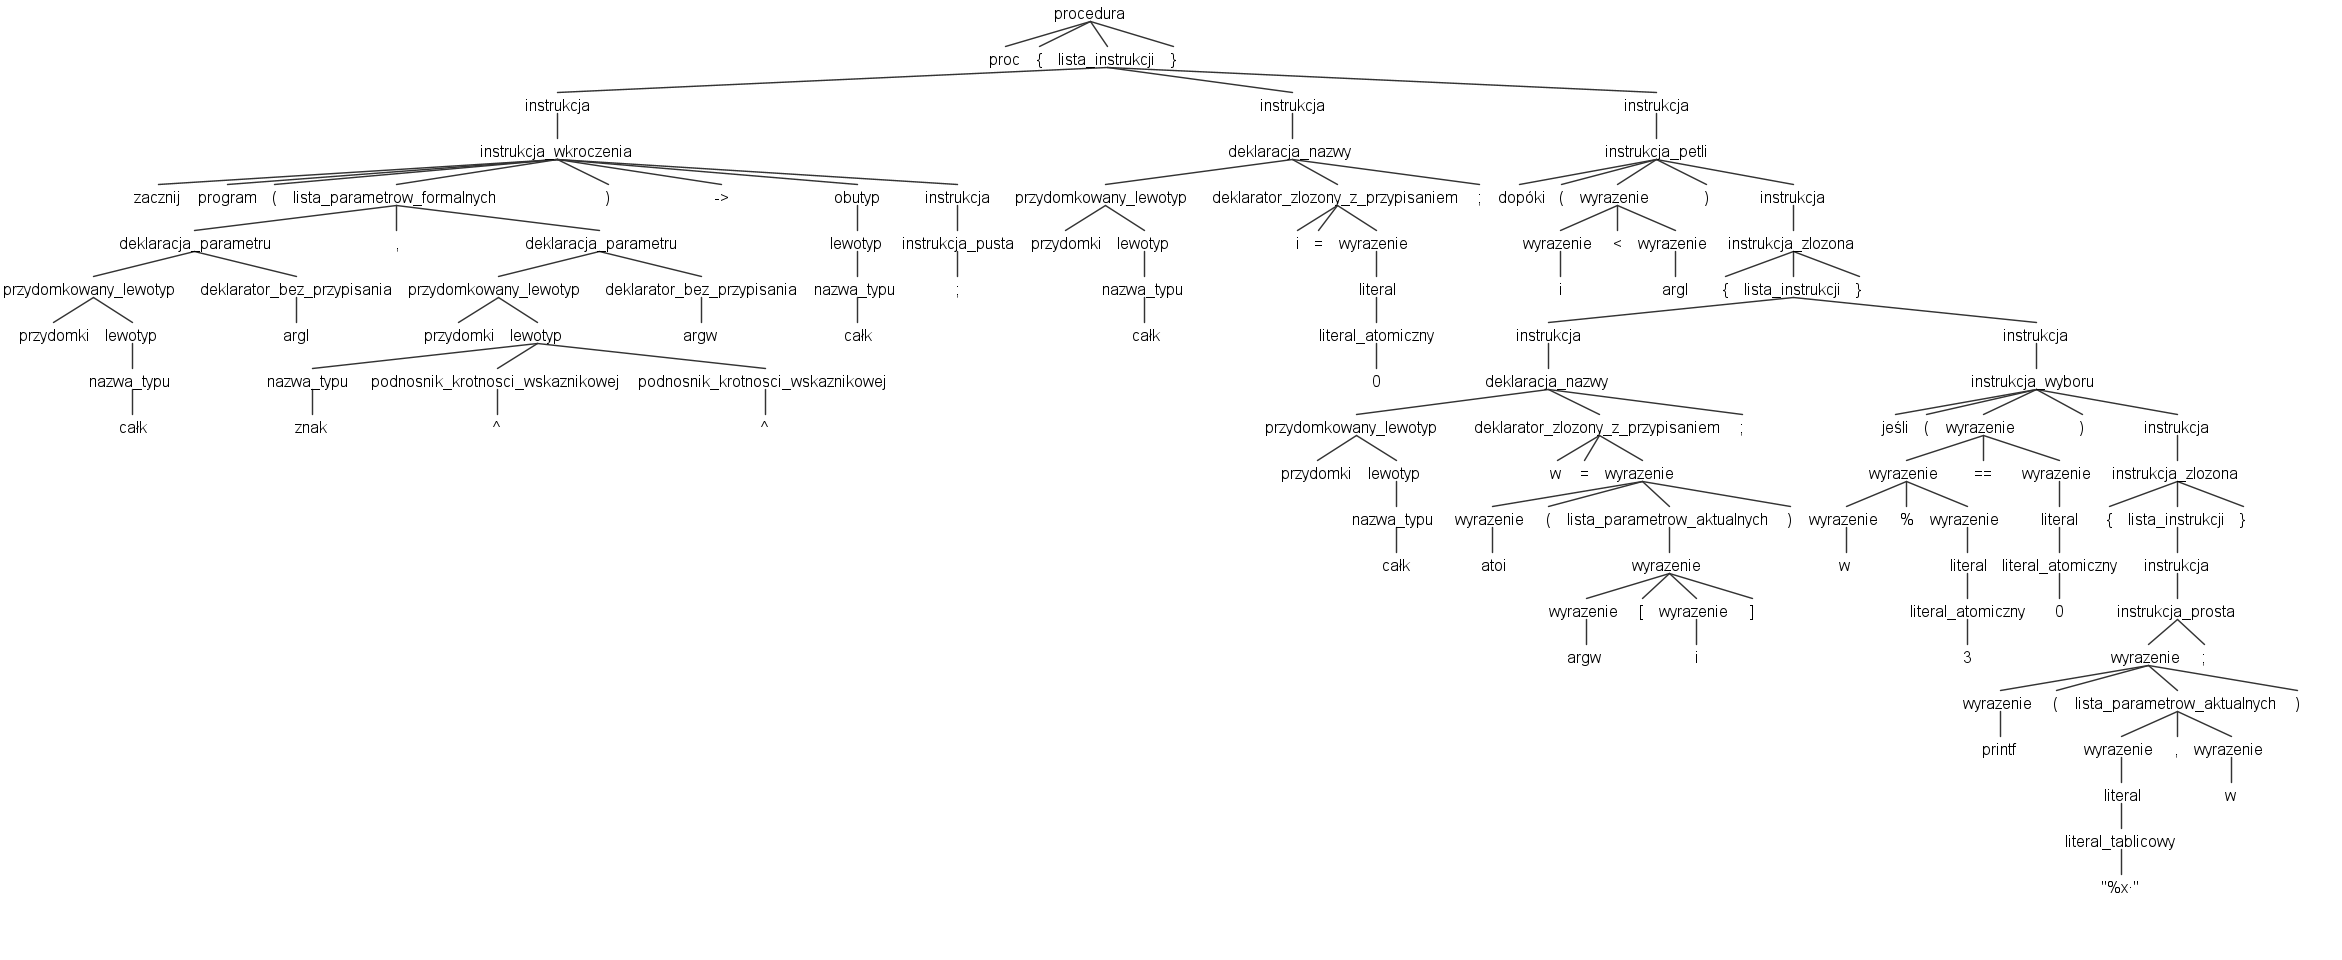
\includegraphics[width=\linewidth]{images/1.progmain/prezifelsePT1.png}
    \caption{Drzewo rozbioru}
    \label{img_pt}
\end{figure}
\end{landscape}

\begin{landscape}
\begin{figure}[p]
    \centering
    \includesvg[width=\linewidth]{images/1.progmain/prz.5.prezentacja_petla_if.ast.svg}
    \caption{Utworzone abstrakcyjne drzewo składniowe}
    \label{img_ast}
\end{figure}
\end{landscape}

\begin{landscape}
\begin{figure}[p]
    \centering
    \includesvg[width=\linewidth]{images/1.progmain/prz.5.prezentacja_petla_if.tpast.svg}
    \caption{Typowane drzewo składniowe}
    \label{img_tpast}
\end{figure}
\end{landscape}
\begin{figure}[H]
    \centering
    \includesvg[width=1.0\textwidth]{images/1.progmain/cfg1.svg}
    \caption{Postać pośrednia LLVM (narysowana w formie grafu przepływu sterowania)}
    \label{img:img_llvm_ctrl_flow}
    %(opt -passes="dot-cfg" -disable-output .\\prz.5.prezentacja_petla_if.ll)
\end{figure}
\newpage%bo rysunek uciekł w kosmos

Wywołuje się potem rekursywnie na w węzłach drzewa rozbioru rozmaite metody ,,visit''. Następuje wtedy przetworzenie deklaracji, wstawienie nazw do zasięgów oraz budowa abstrakcyjnego drzewa składniowego (Rys. \ref{img_ast}).

Kolejnym krokiem jest uruchomienie procedury sprawdzania typów. W jej toku obliczany jest typ każdego węzła i sprawdzane są odpowiednie ograniczenia równości typów. Wyrażenia, gdzie oblicza się adres a nie wartość (lwartości), np. lewe strony operatorów przypisania, są sprawdzane, aby upewnić się, że istotnie posiadają adres w pamięci (a nie są np. stałą). Niekiedy, trzeba wstawiać dodatkowe węzły konwersji, jeśli zezwalają na to reguły konwersji automatycznych, w przeciwnym wypadku trzeba zgłosić błąd. Błędy zawierają numer linii, ponieważ węzły AST zachowują informację o pozycjach w tekście źródłowym węzłów drzewa rozbioru, z których powstały. (Rys. \ref{img_tpast})

Po tych zabiegach, można wygenerować kod. W tym celu na węzłach AST wywołuje się rekursywnie rozmaite metody ,,generate'', które poprzez schematy translacji wywołujące odpowiednio funkcje LLVM C API, tworzą trzecie drzewo - postaci pośredniej LLVM (rys. \ref{img:img_llvm_ctrl_flow}) 
%\marginnote{Obrazek generuje się na innej stronie dlatego zamiast dwukropka należy podac odwołanie do obrazka}
%Rysunek przeniesiony wyżej, by był zaraz po drzewach składniowych

\section{Postać pośrednia LLVM}
Postać pośrednią LLVM zaprojektowano jako uniwersalną reprezentację, używaną zarówno przy kompilacji C jak i C++ w clang. Jej tekstową reprezentację można uzyskać wywołując program clang z przełącznikami ,,-S -emit-llvm''. Wydaje się ona być językiem pomiędzy C/C++ a asemblerem, uproszczonym, pozbawionym na przykład wszelkich automatycznych konwersji, traktującym wszystkie wskaźniki jednako, lecz z drugiej strony posiadając np. wyodrębnione pojęcie funkcji. Najlepiej jednak naturę LLVM IR przedstawia rys.\ref{img:img_llvm_ctrl_flow}, ponieważ LLVM IR stanowi w pierwszym rzędzie drzewiastą reprezentację w roboczej pamięci translatora.

Najwyższym w jej hierarchii jest moduł i zawierać on może wiele funkcji, każda funkcja zawiera listę bloków, a blok listę instrukcji. Każdy blok wszakże musi być ,,domknięty''(sealed), czyli kończyć się instrukcją skoku (warunkowego, bezwarunkowego, lub pośredniego), albo powrotu. Konstruuje się w ten sposób graf przepływu (control flow graph), który jest strukturą niezbędną do przeprowadzania dalszych analiz i optymalizacji\cite{llvm_lang_ref}.

Można zapisać LLVM IR w postaci tekstowej (plików .ll). Jak wspomniano, w przypadku kompilacji C można wywołać "clang -S -emit-llvm plik.c". Zaimplementowany w tej pracy kompilator z kolei wywołuje odpowiednią funkcję w LLVM C API. Dla omawianego powyżej programu, wygenerowana postać pośrednia przedstawia się następująco:

\begin{lstlisting}[
    basicstyle=\scriptsize
]
; ModuleID = 'src\test\java\pl\plpl\prz.5.prezentacja_petla_if'
source_filename = "src\\test\\java\\pl\\plpl\\prz.5.prezentacja_petla_if"

@"napis_%x _8:29-8:33" = global [4 x i8] c"%x \00"

declare i32 @printf(ptr, ...)

declare i32 @atoi(ptr)

define i64 @program(i64 %0, ptr %1) {
wejscie:
  %i = alloca i64, align 8
  %argw = alloca ptr, align 8
  %w = alloca i64, align 8
  %argl = alloca i64, align 8
  store i64 %0, ptr %argl, align 4
  store ptr %1, ptr %argw, align 8
  br label %drugiBlok

drugiBlok:                                        ; preds = %wejscie
  br label %"pierwszy_po_program_4:6-4:52"

"pierwszy_przeskakiwanyprogram_4:6-4:52":         ; No predecessors!
  br label %"pierwszy_po_program_4:6-4:52"

"pierwszy_po_program_4:6-4:52":                   ; preds = %"pierwszy_przeskakiwanyprogram_4:6-4:52", %drugiBlok
  store i64 0, ptr %i, align 4
  br label %"ptl_oblicznie_warunku_5:14-9:4"

"ptl_oblicznie_warunku_5:14-9:4":                 ; preds = %"j_poWarunkowej8:8-8:39", %"pierwszy_po_program_4:6-4:52"
  %i_wt = load i64, ptr %i, align 4
  %argl_wt = load i64, ptr %argl, align 4
  %"opProstai<" = icmp slt i64 %i_wt, %argl_wt
  %"opprostai_rozsz<" = zext i1 %"opProstai<" to i64
  %ptl__zwezenie_dla_warunku = icmp ne i64 %"opprostai_rozsz<", 0
  br i1 %ptl__zwezenie_dla_warunku, label %"pierwszyPetli_5:14-9:4", label %"poPetli_5:14-9:4"

"pierwszyPetli_5:14-9:4":                         ; preds = %"ptl_oblicznie_warunku_5:14-9:4"
  %argw_wt = load ptr, ptr %argw, align 8
  %i_wt1 = load i64, ptr %i, align 4
  %"ind_adr_7:22-7:28" = getelementptr inbounds ptr, ptr %argw_wt, i64 %i_wt1
  %"ind_wt_7:22-7:28" = load ptr, ptr %"ind_adr_7:22-7:28", align 8
  %"call_7:17-7:29" = call i32 @atoi(ptr %"ind_wt_7:22-7:28")
  %"sext7:17-7:29" = sext i32 %"call_7:17-7:29" to i64
  store i64 %"sext7:17-7:29", ptr %w, align 4
  %w_wt = load i64, ptr %w, align 4
  %"opProstai%" = srem i64 %w_wt, 3
  %"opProstai==" = icmp eq i64 %"opProstai%", 0
  %"opprostai_rozsz==" = zext i1 %"opProstai==" to i64
  %j__zwezenie_dla_warunku = icmp ne i64 %"opprostai_rozsz==", 0
  br i1 %j__zwezenie_dla_warunku, label %"j__gdyPrawdziwe_8:8-8:39", label %"j_poWarunkowej8:8-8:39"

"j__gdyPrawdziwe_8:8-8:39":                       ; preds = %"pierwszyPetli_5:14-9:4"
  %w_wt2 = load i64, ptr %w, align 4
  %"call_8:22-8:37" = call i32 (ptr, ...) @printf(ptr @"napis_%x _8:29-8:33", i64 %w_wt2)
  br label %"j_poWarunkowej8:8-8:39"

"j_poWarunkowej8:8-8:39":                         ; preds = %"j__gdyPrawdziwe_8:8-8:39", %"pierwszyPetli_5:14-9:4"
  br label %"ptl_oblicznie_warunku_5:14-9:4"

"poPetli_5:14-9:4":                               ; preds = %"ptl_oblicznie_warunku_5:14-9:4"
  ret i64 0
}

define i32 @main(i32 %0, ptr %1) {
main_plpl_entry:
  %argc_sext = sext i32 %0 to i64
  %wywolanie_f_program = call i64 @program(i64 %argc_sext, ptr %1)
  %ret_main_plpl = trunc i64 %wywolanie_f_program to i32
  ret i32 %ret_main_plpl
}

\end{lstlisting}

Wyraźnie widać, że nie jest to język przeznaczony do recepcji przez osoby postronne. Poleganie na jego tekstowej postaci może okazać się zgubne, ponieważ sam LLVM ulega ciągłym przemianom i kod pośredni, jako format wewnętrzny, niezwiązany żadnym standardem zmienia się z czasem. Sama postać tekstowa jest również niedostatecznie udokumentowana i według mnie zrozumienie jej bez wcześniejszej znajomości mechanizmów LLVM i skuteczne użycie jest w zasadzie niemożliwe. Z kolei API jest wytłumaczone szczegółowo i przystępnie na przykładzie w znakomitym samouczku rozwijanym przez twórców LLVM\cite{kalleidoscope}, choć w moim wypadku pożyteczny okazał się również osobny podręcznik\cite{llvm_nacke_textbook}.

Podstawowym punktem odniesienia  jest oczywiście oficjalna dokumentacja\cite{llvm_lang_ref}. Wyczerpująco opisuje ona wszystkie istotne aspekty funkcjonowania tego systemu. Jedynym zastrzeżeniem, jakie autor tej pracy jest w stanie wobec niej wysunąć, jest to, że z biegiem czasu, powiększyła się znacznie o opisy mnogich specjalistycznych instrukcji, co czyni z niej bardzo długi dokument i zaciemnia jego strukturę. Piszący te słowa bardzo skorzystał, gdy trafił omyłkowo na starszą wersję dokumentacji, wielokroć krótszą, co eksponowało podstawowe elementy języka i systemu typów.

\section{Wybrane schematy translacji}
Zdecydowałem się na przedrukowanie tutaj niektórych schematów translacji w całości, żeby pokazać charakter interfejsu programistycznego LLVM i moją propozycję jego użycia w Javie (korzystając z JNI). Teksty te mogą się również okazać przydatne dla osoby, która znalazłaby się w sytuacji podobnej do mojej, potrzebując napisać takie schematy, dysponując jednocześnie dość szczupłym zbiorem przykładów, dostępnych w Sieci.

Schemat dla węzła ,,OperacjiProstej'' zawiera w zasadzie całą prostą arytmetykę.

\begin{lstlisting}[basicstyle=\scriptsize]
    public LLVMValueRef _generuj(LLVMContextRef c, LLVMValueRef func, LLVMBuilderRef builder, KontekstGeneracji kg){
        if(lewe.typ() == null || (!lewe.typ().równyFunkcjonalnie(prawe.typ()))){
            throw new WewnętrznyBłąd(String.format("OpProsta:nierówne typy: %s vs %s", lewe.typ(), prawe.typ()));
        }
        LLVMValueRef lewyrejestr = lewe.generuj(c, func, builder, kg);
        LLVMValueRef prawyrejestr = prawe.generuj(c, func, builder, kg);
        if(lewe.typ().jestWskaźnikiem()){
            return switch (opkod){
                case "==" -> LLVMBuildZExt(builder, LLVMBuildICmp(builder, LLVMIntEQ, lewyrejestr, prawyrejestr, "opProstap=="), reprTypuLogicznego(c) , "opprostap_rozsz==");
                case "!=" -> LLVMBuildZExt(builder, LLVMBuildICmp(builder, LLVMIntNE, lewyrejestr, prawyrejestr, "opProstap!="), reprTypuLogicznego(c) , "opprostap_rozsz!=");
                default -> throw new TODOException("Nieznany operand dla wskaźnika:"+opkod);
            };
        }
        if(!lewe.typ().jestAtomiczny()){ throw new TODOException("OpProsta:TylkoAtomiczne!"); }
        if(lewe.typ().jestCałkowity()){
            return switch (opkod) {
                case "+" -> LLVMBuildAdd(builder, lewyrejestr, prawyrejestr, "opProstai+");
                case "-" -> LLVMBuildSub(builder, lewyrejestr, prawyrejestr, "opProstai-");
                case "*" -> LLVMBuildMul(builder, lewyrejestr, prawyrejestr, "opProstai*");
                case "/" -> LLVMBuildSDiv(builder, lewyrejestr, prawyrejestr, "opProstai/");
                case "%" -> LLVMBuildSRem(builder, lewyrejestr, prawyrejestr, "opProstai%");
                case "==" -> LLVMBuildZExt(builder, LLVMBuildICmp(builder, LLVMIntEQ, lewyrejestr, prawyrejestr, "opProstai=="), reprTypuLogicznego(c) , "opprostai_rozsz==");
                case "!=" -> LLVMBuildZExt(builder, LLVMBuildICmp(builder, LLVMIntNE, lewyrejestr, prawyrejestr, "opProstai!="), reprTypuLogicznego(c) , "opprostai_rozsz!=");
                case ">" -> LLVMBuildZExt(builder, LLVMBuildICmp(builder, LLVMIntSGT, lewyrejestr, prawyrejestr, "opProstai>"), reprTypuLogicznego(c) , "opprostai_rozsz>");
                case ">=" -> LLVMBuildZExt(builder, LLVMBuildICmp(builder, LLVMIntSGE, lewyrejestr, prawyrejestr, "opProstai>="), reprTypuLogicznego(c) , "opprostai_rozsz>=");
                case "<" -> LLVMBuildZExt(builder, LLVMBuildICmp(builder, LLVMIntSLT, lewyrejestr, prawyrejestr, "opProstai<"), reprTypuLogicznego(c) , "opprostai_rozsz<");
                case "<=" -> LLVMBuildZExt(builder, LLVMBuildICmp(builder, LLVMIntSLE, lewyrejestr, prawyrejestr, "opProstai<="), reprTypuLogicznego(c) , "opprostai_rozsz<=");
                case "&&" -> LLVMBuildZExt(builder,
                                LLVMBuildAnd(builder,
                                        LLVMBuildTruncOrBitCast(builder, lewyrejestr, LLVMInt1TypeInContext(c), "&&ltrunc"),
                                        LLVMBuildTruncOrBitCast(builder, prawyrejestr, LLVMInt1TypeInContext(c), "&&rtrunc"),
                                    "&&and"),
                                reprTypuLogicznego(c), "&&zext");
                case "||" -> LLVMBuildZExt(builder,
                        LLVMBuildOr(builder,
                                LLVMBuildTruncOrBitCast(builder, lewyrejestr, LLVMInt1TypeInContext(c), "||ltrunc"),
                                LLVMBuildTruncOrBitCast(builder, prawyrejestr, LLVMInt1TypeInContext(c), "||rtrunc"),
                                "||or"),
                        reprTypuLogicznego(c), "||zext");
                default -> throw new TODOException("Nieznany operand całkowity:"+opkod);
            };
        }
        if(lewe.typ().jestZmiennoiprzecinkowy()) {
            return switch (opkod) {
                case "+" -> LLVMBuildFAdd(builder, lewyrejestr, prawyrejestr, "opProstaf+");
                case "-" -> LLVMBuildFSub(builder, lewyrejestr, prawyrejestr, "opProstaf-");
                case "*" -> LLVMBuildFMul(builder, lewyrejestr, prawyrejestr, "opProstaf*");
                case "/" -> LLVMBuildFDiv(builder, lewyrejestr, prawyrejestr, "opProstaf/");
                case "==" -> LLVMBuildZExt(builder, LLVMBuildFCmp(builder, LLVMRealOEQ, lewyrejestr, prawyrejestr, "opProstaf=="), reprTypuLogicznego(c) , "opprostaf_rozsz==");
                case "!=" -> LLVMBuildZExt(builder, LLVMBuildFCmp(builder, LLVMRealONE, lewyrejestr, prawyrejestr, "opProstaf!="), reprTypuLogicznego(c) , "opprostaf_rozsz!=");
                case ">" -> LLVMBuildZExt(builder, LLVMBuildFCmp(builder, LLVMRealOGT, lewyrejestr, prawyrejestr, "opProstaf>"), reprTypuLogicznego(c) , "opprostaf_rozsz>");
                case ">=" -> LLVMBuildZExt(builder, LLVMBuildFCmp(builder, LLVMRealOGE, lewyrejestr, prawyrejestr, "opProstaf>="), reprTypuLogicznego(c) , "opprostaf_rozsz>=");
                case "<" -> LLVMBuildZExt(builder, LLVMBuildFCmp(builder, LLVMRealOLT, lewyrejestr, prawyrejestr, "opProstaf<"), reprTypuLogicznego(c) , "opprostaf_rozsz<");
                case "<=" -> LLVMBuildZExt(builder, LLVMBuildFCmp(builder, LLVMRealOLE, lewyrejestr, prawyrejestr, "opProstaf<="), reprTypuLogicznego(c) , "opprostaf_rozsz<=");
                default -> throw new TODOException("Nieznany operand zmiennoprzecinkowy:"+opkod);
            };
        }
        kg.jk.katastrofa("Brak zdefiniowanej operacji prostej dla operandów typu: "+lewe.typ(), this.msc); return null;
    } 
\end{lstlisting}
Schemat dla pętli pokazuje, że o ile nie zadba się o odpowiednie ułożenie bloków, to schemat wprawdzie będzie działał, lecz zrzucony do pliku tekst postaci pośredniej będzie dl człowieka nieczytelny.
\lstset{
    escapechar=`,
    breaklines=true
}
\begin{lstlisting}[basicstyle=\scriptsize]
/*  ------>:obliczanie_warunku
    |       ...
    ^       %wyr_warunku = icmp ...
    |       br i1 %wyr_warunku, label %pierwszy_pętli, label %po_pętli
    |                                   |                       |
    ^   |--------------------------------                       |
    | |-+--------------------------------------------------------
    | | |-->:pierwszy_petli
    | V     ...
    ^ |     ...
    | |     ...
    | V     (:jakis_ostatni_pętli)?
    | |     ....
    --+---<-br %obliczanie_warunku
      |
      |---->:po_pętli
            ...
*/
    @Override
    public LLVMValueRef _generuj(LLVMContextRef c, LLVMValueRef func, LLVMBuilderRef builder, KontekstGeneracji kg) {
        sprawdźBlok(builder);
        //pętla ma skakać do początku obliczania warunku za każdym razem, więc potrzebujemy wstawić nowy blok, dodac skok bezwarunkowy z ostatniego do tego nwego.
        LLVMBasicBlockRef oblicznieWarunku = LLVMAppendBasicBlockInContext(c, func, "ptl_oblicznie_warunku_"+msc);
        LLVMMoveBasicBlockAfter(oblicznieWarunku, LLVMGetInsertBlock(builder));//na prawdziwym końcu funkcji coś może być już dołozone przez węzły wyżej
        LLVMBuildBr(builder, oblicznieWarunku);
        LLVMPositionBuilderAtEnd(builder, oblicznieWarunku);

        LLVMValueRef liczbaWarunku = warunek.generuj(c, func, builder, kg); sprawdźBlok(builder);
        assert liczbaWarunku != null;
        LLVMValueRef wyrWarunku = LLVMBuildICmp(builder, LLVMIntNE, liczbaWarunku, zeroTypuLogicznego(c), "ptl__zwezenie_dla_warunku");

        LLVMBasicBlockRef pierwszyWPętli = LLVMAppendBasicBlockInContext(c, func, "pierwszyPetli_"+msc);
        LLVMMoveBasicBlockAfter(pierwszyWPętli, oblicznieWarunku);//na prawdziwym końcu funkcji coś może być już dołozone przez węzły wyżej

        //Potrzebujemy referencji do bloku po pętli, by można było użyć break w środku pętli
        LLVMBasicBlockRef poPętli = LLVMAppendBasicBlockInContext(c, func, "poPetli_"+msc);
        LLVMMoveBasicBlockAfter(poPętli, pierwszyWPętli);

        LLVMBuildCondBr(builder, wyrWarunku, pierwszyWPętli, poPętli);

        //piszemy ciało pętli
        LLVMPositionBuilderAtEnd(builder, pierwszyWPętli);
        kg.stosPętli.push(new Etykietki(pierwszyWPętli, poPętli));//żeby break i continue miały się do czego odwoływać

        ciało.generuj(c, func, builder, kg); sprawdźBlok(builder);

        kg.stosPętli.pop();

        //domykamy pierwszyWPętli/któregos z jego następników
        LLVMBuildBr(builder, oblicznieWarunku);
        //przenosimy się za pętlę
        LLVMPositionBuilderAtEnd(builder, poPętli); sprawdźBlok(builder);
        return null;
    }
\end{lstlisting}

Schematy dla instrukcji warunkowych, wywołań są w zasadzie podobne i z racji częstego opisywania w literaturze, nie będą już cytowane.
\newpage

\section{Weryfikacja generacji kodu}
Oczekuje się od kompilatorów daleko większej niezawodności niż od ,,zwykłych'' aplikacji\cite{waite_goos}. Użytkownik języka nie zna zazwyczaj programu kompilatora i nie orientuje się szczegółowo w jego działaniu. Ostatnią rzeczą, jakiej spodziewa się programista języka wysokiego poziomu, próbując naprawić błąd w swym programie, jest defekt samego kompilatora. Z powodu tak dużej odpowiedzialności, w konstrukcji kompilatorów stawia się wysokie wymagania jakościowe i jednym ze sposobów ich wypełnienia są z pewnością szerokie testy, w szczególności automatyczne.

\subsection{Testy jednostkowe i wizualna reprezentacja AST}
Stworzenie przydatnych testów jednostkowych, napotkało w tym projekcie dwa zasadnicze problemy. Po pierwsze, wynikiem wielu powszechnych operacji są drzewa, a Java nie ma wbudowanego dopasowywania struktur (pattern matching), co czyni każdy kod sprawdzający strukturę drzewa bardzo nieczytelnym i kosztownym w utrzymaniu. Dodatkowo, w większości wypadków wymagany jest szerszy kontekst. Wewnątrz autorskiego kodu analizy semantycznej, da się utworzyć sztuczny kontekst, na potrzeby testów, choć jego odrębność, może negować całe przedsięwzięcie i czyni je kosztownym. Z kolei, wywołań API LLVM nie da się testować osobno - nie można utworzyć bloku, nie mając funkcji, funkcji nie mając modułu, a modułu bez utworzenia kontekstu LLVM.

W związku z tym, klasyczne testy jednostkowe znalazły jedynie ograniczone zastosowanie, np. przy testowaniu działania wyrażeń określających typ, gdzie da się wywołać parser przyjmując inny symbol startowy i sprawdzić równość wygenerowanego typu z oczekiwanym. O wiele bardziej użyteczne, zwłaszcza na etapie intensywnego rozwoju programu, było wizualne sprawdzanie generowanych drzew, przy pomocy prezentowanych powyżej diagramów AST. Każdy węzeł drzewa zaopatrzyłem w metodę zwracającą jego reprezentację w języku opisu grafów DOT, programu graphviz, który to program jest następnie wywoływany na rekursywnie zbudowanej reprezentacji, celem wygenerowania obrazka wektorowego (svg). Tekstowe przedstawienia AST stają się szybko nieczytelne już dla małych przykładów, a graficzna reprezentacja zawiera większość istotnej informacji i umożliwiają wizualną kontrolę dużo bardziej rozbudowanych konstrukcji. Zamieszczone wcześniej przykłady drzew składniowych - rys. \ref{img_ast}, \ref{img_tpast} były przykładami takich reprezentacji, bezpośrednio zaczerpniętymi z testów.

\subsection{Testy aplikacyjne - działające programy}
Oczywiście ostatecznym testem jest skompilowanie programu i sprawdzenie, czy wynikowy obraz wykonywalny, po uruchomieniu działa zgodnie z oczekiwaniami (choć to ostatnie można w praktyce sprawdzić jedynie dla bardzo prostych programów, bowiem przestrzeń możliwych wejść i wyjść rośnie bardzo szybko wraz ze złożonością kodu źródłowego). Drugim rodzajem testu, wielokroć prostszym do automatyzacji jest próba skompilowania programu błędnego i sprawdzenie, czy translator wygenerował odpowiednie komunikaty.

Do tego ostatniego celu uznałem uruchamianie programu kompilatora z zewnątrz za zbyteczne, utworzyłem osobny sposób wywołania kompilatora, z samej Javy, na zasadzie przypominającej API. Dzięki temu, poruszając się w środowisko Javy, test taki, zamiast przetwarzać tekst błędów, może sprawdzić równość i strukturę samych obiektów wygenerowanych zdarzeń, co pomija etap parsowania wyjścia samego kompilatora.

Udało mi się uzyskać zbiór programów testujących najważniejsze aspekty funkcjonowania translatora i błędy, które może zgłosić. Jednym z najistotniejszych celów utrzymywania zbioru takich testów, jest oczywiście testowanie regresyjne - aby zmiana w kodzie translatora ,,psująca'' coś, odzwierciedliła się natychmiast w automatycznych testach. Z pewnym zadowoleniem stwierdzam, że zbiór testów w tym projekcie już zaczął pełnić taką funkcję.
%pomimo braku testów pierwszego rodzaju - już dopisałem!
%tu wrzucić jakieś przykłady uruchomionych programów????

\subsection{Weryfikacja poprawności generowanego obrazu wykonywalnego}
Dla niemal każdego programu, poza najbardziej trywialnymi, nie sposób przetestować wszystkich możliwych kombinacji wejść Użycie zaś programu typu \textit{fuzzer} wykracza poza zakres tej pracy, zresztą i tak generują one jedynie probabilistyczną próbkę przestrzeni napisów wejściowych. Ażeby skontrolować działanie całego procesu translacji, trzeba zatem przyjrzeć się również jego rzeczywistemu efektowi - obrazowi binarnemu. Dość łatwo uzyskać kod asemblerowy - wystarczy skompilować za pomocą clanga wygenerowany plik.ll z przełącznikiem -S, Dla poprzednio omawianego programu pełny wynik przedstawia się następująco:

\begin{lstlisting}[basicstyle=\scriptsize]
	.text
	.def	@feat.00;
	.scl	3;
	.type	0;
	.endef
	.globl	@feat.00
.set @feat.00, 0
	.file	"prz.5.prezentacja_petla_if"
	.def	program;
	.scl	2;
	.type	32;
	.endef
	.globl	program                         # -- Begin function program
	.p2align	4, 0x90
program:                                # @program
.seh_proc program
# %bb.0:                                # %wejscie
	subq	$72, %rsp
	.seh_stackalloc 72
	.seh_endprologue
	movq	%rcx, 40(%rsp)
	movq	%rdx, 56(%rsp)
# %bb.1:                                # %drugiBlok
	jmp	.LBB0_2
.LBB0_2:                                # %"pierwszy_po_program_4:6-4:52"
	movq	$0, 64(%rsp)
.LBB0_3:                                # %"ptl_oblicznie_warunku_5:14-9:4"
                                        # =>This Inner Loop Header: Depth=1
	movq	64(%rsp), %rax
	cmpq	40(%rsp), %rax
	setl	%al
	andb	$1, %al
	movzbl	%al, %eax
                                        # kill: def $rax killed $eax
	cmpq	$0, %rax
	je	.LBB0_7
# %bb.4:                                # %"pierwszyPetli_5:14-9:4"
                                        #   in Loop: Header=BB0_3 Depth=1
	movq	56(%rsp), %rax
	movq	64(%rsp), %rcx
	movq	(%rax,%rcx,8), %rcx
	callq	atoi
	cltq
	movq	%rax, 48(%rsp)
	movq	48(%rsp), %rax
	movl	$3, %ecx
	cqto
	idivq	%rcx
	cmpq	$0, %rdx
	sete	%al
	andb	$1, %al
	movzbl	%al, %eax
                                        # kill: def $rax killed $eax
	cmpq	$0, %rax
	je	.LBB0_6
# %bb.5:                                # %"j__gdyPrawdziwe_8:8-8:39"
                                        #   in Loop: Header=BB0_3 Depth=1
	movq	48(%rsp), %rdx
	leaq	"napis_%x _8:29-8:33"(%rip), %rcx
	callq	printf
.LBB0_6:                                # %"j_poWarunkowej8:8-8:39"
                                        #   in Loop: Header=BB0_3 Depth=1
	jmp	.LBB0_3
.LBB0_7:                                # %"poPetli_5:14-9:4"
	xorl	%eax, %eax
                                        # kill: def $rax killed $eax
	addq	$72, %rsp
	retq
	.seh_endproc
                                        # -- End function
	.def	main;
	.scl	2;
	.type	32;
	.endef
	.globl	main                            # -- Begin function main
	.p2align	4, 0x90
main:                                   # @main
.seh_proc main
# %bb.0:                                # %main_plpl_entry
	subq	$40, %rsp
	.seh_stackalloc 40
	.seh_endprologue
	movslq	%ecx, %rcx
	callq	program
                                        # kill: def $eax killed $eax killed $rax
	nop
	addq	$40, %rsp
	retq
	.seh_endproc
                                        # -- End function
	.data
	.globl	"napis_%x _8:29-8:33"           # @"napis_%x _8:29-8:33"
"napis_%x _8:29-8:33":
	.asciz	"%x "

	.addrsig
	.addrsig_sym printf
	.addrsig_sym atoi
	.addrsig_sym program
	.addrsig_sym "napis_%x _8:29-8:33"

\end{lstlisting}
Kod wygenerowany przez automat nie byłby miłą lekturą nawet dla doświadczonego programisty asemblerowego, a jak juz powiedziano na początku tego tekstu, znajomość asemblera na takim poziomie, by przeczytać powyższy wydruk i orzec z niewzruszoną pewnością o jego poprawności (lub niepoprawności), jako przekładu kodu źródłowego, to rzadka w dzisiejszych czasach umiejętność. Na szczęście istnieje prostszy sposób na weryfikację, i to nie sztucznie wygenerowanego asemblera, lecz bezpośrednio obrazu bianrnego, wyprodukowanego przez llvm (pliku .o, lub po konsolidacji, w zależności od systemu ELF lub EXE).

\subsection{Dekompilator Ghidra}
Amerykańska Agencja Bezpieczeństwa Narodowego oddała wielką przysługę postronnym, udostępniając za darmo jedno ze swych narzędzi - dekompilator Ghidra\cite{ghidra}. Program tego rodzaju analizuje obraz wykonywalny i próbuje odtworzyć kod w języku wysokiego poziomu. Nie jest to oczywiście możliwe całkowicie - proces kompilacji jest stratną konwersją na wielu etapach, jednak interfejsy binarne, konwersje wywołań są na tyle blisko języka C, że można próbować częściowo go odtworzyć. 

Rekonstrukcja taka, pozbawiona będzie wszak wielu informacji, przede wszystkim nazw zmiennych, gdy pełne tablice symboli nie są obecne, co jest częstym zwyczajem podczas zwyczajnej kompilacji (nie sprofilowanej do debugowania). Osoba podejmująca się inżynierii wstecznej takiego obrazu, musi wtedy sama wydedukować przeznaczenie poszczególnych zmiennych i nadać im przypuszczalne nazwy.

Poniżej znajduje się zrzut ekranu, pokazujący efekt zastosowania Ghidry na obrazie binarnym omawianego programu.
\begin{figure}[h]
    \centering
    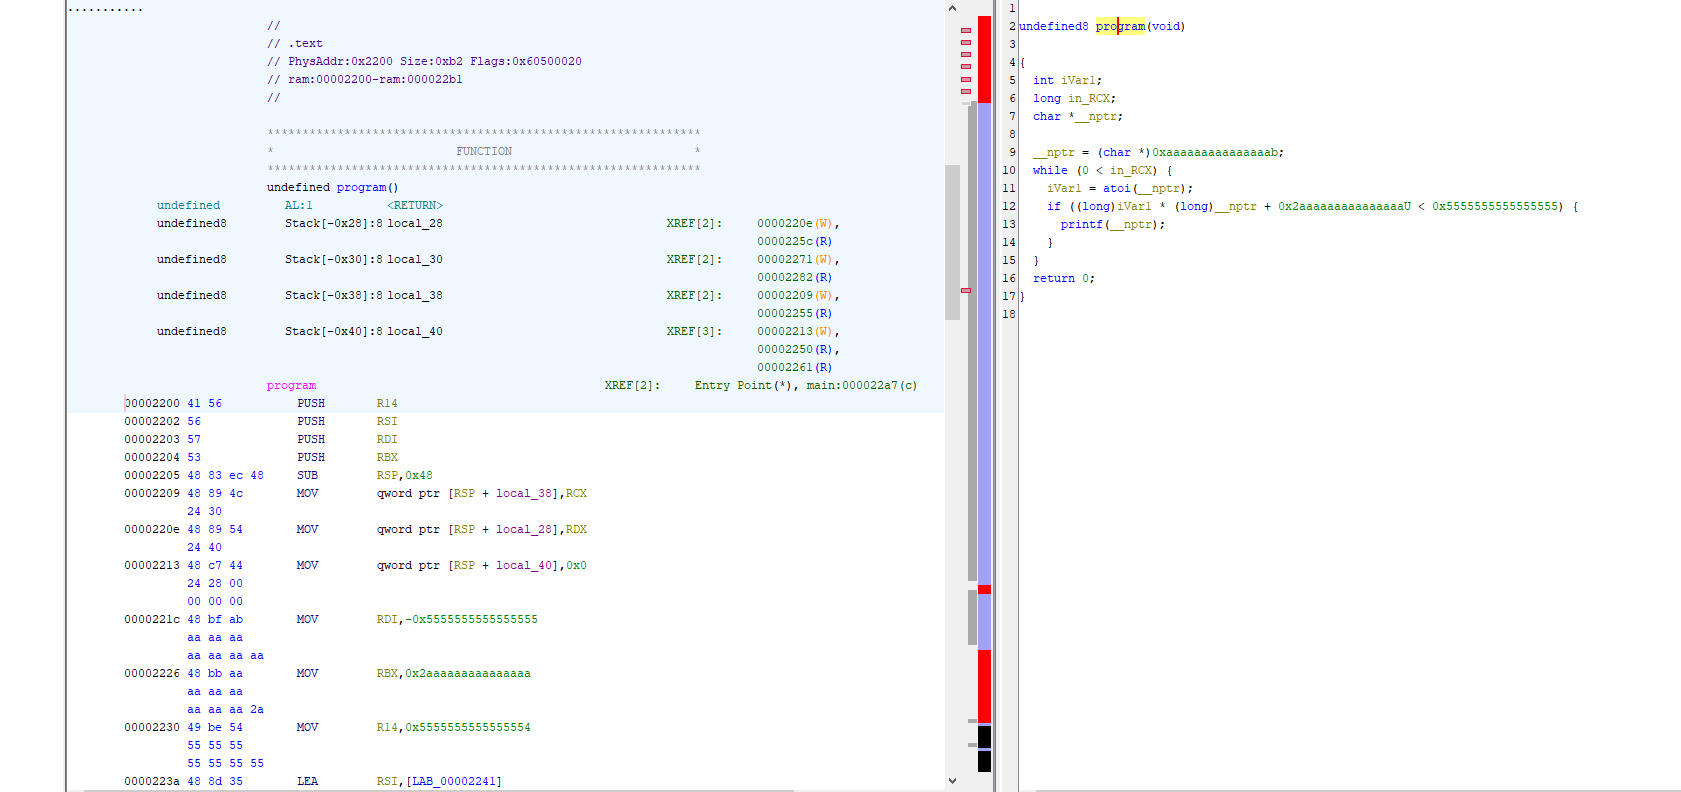
\includegraphics[width=1.3\textwidth]{images/1.progmain/ghidra1.png}
    \caption{Widok dekompilacji w programie GHIDRA}
\end{figure}

W lewym panelu znajduje się zdesamblewany kod, odpowiadający zamieszczonemu powyżej (Ghidra używa wszak składni Intela, różnej od GNU ASM, produkowanej domyślnie przez clanga). Po prawej stronie widnieje przypuszczalna rekonstrukcja programu w języku C. Poprawnie zrekonstruowano funkcję ,,program'' (akurat publiczne symbole zawsze znajdują się w obrazach), i ewidentnie zawiera ona pętlę i warunek, w układzie odpowiadającym kodowi źródłowemu. 

Za artefakty w postaci nieoczekiwanych stałych, oraz niepełnego wywołania wariadycznej funkcji printf, można obarczyć konwencję wywołań cdecl na IA-64, gdzie pierwsze argumenty funkcji znajdują się w rejestrach i dekompilator boryka się z właściwą ich interpretacją.
Niemniej jednak zweryfikowaliśmy, że cała maszyneria translatora istotnie działa i produkuje odpowiadający programowi źródłowemu, dość zgrabny kod, z pewnością nie ,,rażąco nieefektywny''.

\section{Sposób translacji wielokrotnych punktów wejściowych}
W tym miejscu wywodu pozostaje już tylko jeden punkt do objaśnienia - jak w przedstawionym stosie technologicznym zaimplementowano translację wielokrotnych punktów wejściowych. W prototypie, operując asemblerem, można było swobodnie rozsadzić zwyczajową strukturę kodu funkcji, umieszczając w jednej sekcji kodu kilka wołanych symboli. LLVM jednak operuje już wszak na podstawowym poziomie pojęciem funkcji, z jednym punktem wejściowym i zmienić tego nie sposób. Na szczęście, podobny problem napotkali już wcześniej autorzy rozmaitych transpilerów z FORTRANU (posiadająego ,,alternate entry points'') do C (posiadającego wyłącznie zwykłe funkcje)\cite{gpp_entry_points}. Rozwiązanie podobne do stosowanego przez f2c zostało użyte w tym projekcie i zostanie pokrótce przedstawiona jego racjonalizacja.

W poniższym wywodzie zostanie jako przykład użyta trywialna procedura z dwoma punktami wejściowymi:
\begin{lstlisting}
proc {
tu proporcjonalna(całk a, całk x) -> całk;
	całk b=0;
	printf("\nproporcjonalna %lld %lld %lld",a,x,b);
tu liniowa(całk a, całk b, całk x) -> całk;
	printf("\nliniowa %lld %lld %lld",a,x,b);
	zwróć a*x + b;
}
\end{lstlisting}

\subsection{Wymagania wobec generowanego kodu}
Pierwszą obserwacją, jaką musimy poczynić jest to, że dla każdego punktu wejściowego chcemy umieścić w obrazie wykonywalnym symbol o identycznej nazwie, który można wywołać, stosując się do konwencji wywołań cdecl i do sygnatury punktu wejściowego obecnej w kodzie źródłowym (zaprojektowany język jest na tyle bliski C, że przekształcenie sygnatury w nim do C nie powinno nastręczać trudności). Wymagamy tego, podtrzymując konsekwencje pierwotne założenie kompatybilności z C ABI. Powinniśmy nie tylko móc korzystać z biblioteki standardowej C, nie tylko z innych bibliotek, lecz móc swobodnie linkować skompilowany kod w projektowanym języku z innymi obiektami binarnymi. Musząc używać w LLVM funkcji, nie mamy innego wyjścia, jak wygenerować po jednej funkcji pośredniczącej dla każdego punktu wejściowego. Ma to dodatkową zaletę - naturalnie rozwiązuje problem przestawiania parametrów, ponieważ różne punkty wejściowe mogą mieć parametry formalne ułożone w różnej kolejności (jak i niektóre nieobecne).

\subsection{Schemat translacji}
Generujemy więc funkcje pośredniczące, z których każda woła potem właściwą funkcję, której sygnatura jest sumą wszystkich możliwych parametrów wejściowych. Gdy już sterowanie znajdzie się w tej wewnętrznej procedurze, trzeba go natychmiast przemieścić we właściwe miejsce. Naturalne wydaje się użycie instrukcji switch w połączeniu z goto. W języku C można by zapisać całą konstrukcję w następujący sposób):
\begin{lstlisting}
#define WE_PROPORCJONALNA 1
#define WE_LINIOWA 2
double rozdzielacz(int we, double a, double x, double b)
{
	switch(we)
	{
    	case WE_PROPORCJONALNA: goto we_proporcjonalna;
    	case WE_LINIOWA: goto we_liniowa;
	}
    
	we_proporcjonalna:
	b=0.0;
	printf("\nproporcjonalna %lld %lld %lld",a,x,b);
    
	we_liniowa:
	printf("\nliniowa %lld %lld %lld",a,x,b);
	return a*x + b;
}

double proporcjonalna(double a, double x)
{
	return rozdzielacz(WE_PROPORCJONALNA, a,x,0.0);
}
double we_liniowa(double a, double b, double x)
{
	return rozdzielacz(WE_LINIOWA, a,x,b);
}
\end{lstlisting}
Rozdzielacz otrzymuje jako pierwszy parametr wartość wyliczeniową, określającą, gdzie ma wpierw przeskoczyć sterowanie.
Podobno w podobny sposób działa f2c\cite{gpp_entry_points}. Możemy jednak zauważyć, że te wartości wyliczeniowe w istocie są niepotrzebne, ponieważ znamy podczas kompilacji dokładnie adresy, do których skakać należy, Moglibyśmy jako pierwszy argument przekazać sam adres i dokonać do niego pośredniego skoku. Do tej pory też wykonywany jest skok niebezpośredni, adres jednak musi zostać najpierw wydobyty z tablicy skoków, generowanej dla switch, indeksowanej wartością wyliczeniową. Używając rozszerzeń C gcc - operatora \&\& do pobierania adresów etykiet oraz składni z gwiazdką do skoków pośrednich, moglibyśmy spróbować wyeliminować pośredników:
\begin{lstlisting}
double rozdzielacz(void* we, double a, double x, double b)
{
	goto *we;
    
	we_proporcjonalna:
	b=0.0;
	printf("\nproporcjonalna %lld %lld %lld",a,x,b);

	we_liniowa:
	printf("\nliniowa %lld %lld %lld",a,x,b);
	return a*x + b;
}

double proporcjonalna(double a, double x)
{
	return rozdzielacz(&&we_proporcjonalna, a,x,0.0);
}
double we_liniowa(double a, double b, double x)
{
	return rozdzielacz(&&we_liniowa, a,x,b);
}
\end{lstlisting}
Próba skompilowania skończy się jednak błędami:
\begin{lstlisting}
gcc -c .\prz.4.c.dwuwejsciowa.c
.\prz.4.c.dwuwejsciowa.c: In function 'proporcjonalna':
.\prz.4.c.dwuwejsciowa.c:12:5: error: label 'we_proporcjonalna' used but not defined
 	return rozdzielacz(&&we_proporcjonalna, a,x,0.0);
 	^
.\prz.4.c.dwuwejsciowa.c: In function 'we_liniowa':
.\prz.4.c.dwuwejsciowa.c:16:5: error: label 'we_liniowa' used but not defined
 	return rozdzielacz(&&we_liniowa, a,x,b);
\end{lstlisting}
Etykiety do których chcemy wykonać skok, znajdują się wewnątrz funkcji rozdzielacza, a chcemy uzyskać ich adresy poza nią,  w funkcjach pośredniczących. Reguły zasięgów w języku C wykluczają użycie takiej konstrukcji. Okazuje się jednak, że odpowiadający im schemat w kodzie pośrednim LLVM działa, gdyż backend nie wymusza zasięgów leksykalnych, a referencje do bloków w funkcji są ważne również poza nią (Przynajmniej w LLVM 17).
\begin{lstlisting}
define i64 @rozdzielacz_od_proporcjonalna_do_liniowa(ptr %0, i64 %1, i64 %2, i64 %3) {
wejscie:
  %a = alloca i64, align 8
  %x = alloca i64, align 8
  %b = alloca i64, align 8
  store i64 %1, ptr %a, align 4
  store i64 %2, ptr %x, align 4
  store i64 %3, ptr %b, align 4
  indirectbr ptr %0, [label %"pierwszy_przeskakiwanyproporcjonalna_4:4-4:50", label %"pierwszy_przeskakiwanyliniowa_7:4-7:51"]
[... pominięto dalsze bloki rozdzielacza ...]

define i64 @proporcjonalna(i64 %0, i64 %1) {
"posrednik_proporcjonalna_4:4-4:50":
  %wywolanie_rozdzielacza_od_proporcjonalna_do_liniowa = call i64 @rozdzielacz_od_proporcjonalna_do_liniowa(ptr blockaddress(@rozdzielacz_od_proporcjonalna_do_liniowa, %"pierwszy_przeskakiwanyproporcjonalna_4:4-4:50"), i64 %0, i64 %1, i64 0)
  ret i64 %wywolanie_rozdzielacza_od_proporcjonalna_do_liniowa
}

define i64 @liniowa(i64 %0, i64 %1, i64 %2) {
"posrednik_liniowa_7:4-7:51":
  %wywolanie_rozdzielacza_od_proporcjonalna_do_liniowa = call i64 @rozdzielacz_od_proporcjonalna_do_liniowa(ptr blockaddress(@rozdzielacz_od_proporcjonalna_do_liniowa, %"pierwszy_przeskakiwanyliniowa_7:4-7:51"), i64 %0, i64 %2, i64 %1)
  ret i64 %wywolanie_rozdzielacza_od_proporcjonalna_do_liniowa
}
\end{lstlisting}
Powyższy schemat wymaga użycia rzadko spotykanej instrukcji LLVM IR - indirectbr. Aby nie uniemożliwić analizy przepływu, wymaga ona wyczerpującej listy adresów wszystkich bloków, do której może ona prowadzić. Nie stanowi to jednak w tym przypadku problemu, bo naturalnie posiadamy listę wszystkich punktów wejściowych w danej procedurze.

Ciekawym ćwiczeniem jest analiza wyniku kompilacji powyższego programu za pomocą wspomnianego dekompilatora.
Widzimy, że funkcja pośrednicząca wygenerowana została zgodnie z oczekiwaniami.
\begin{figure}[H]
    \centering
    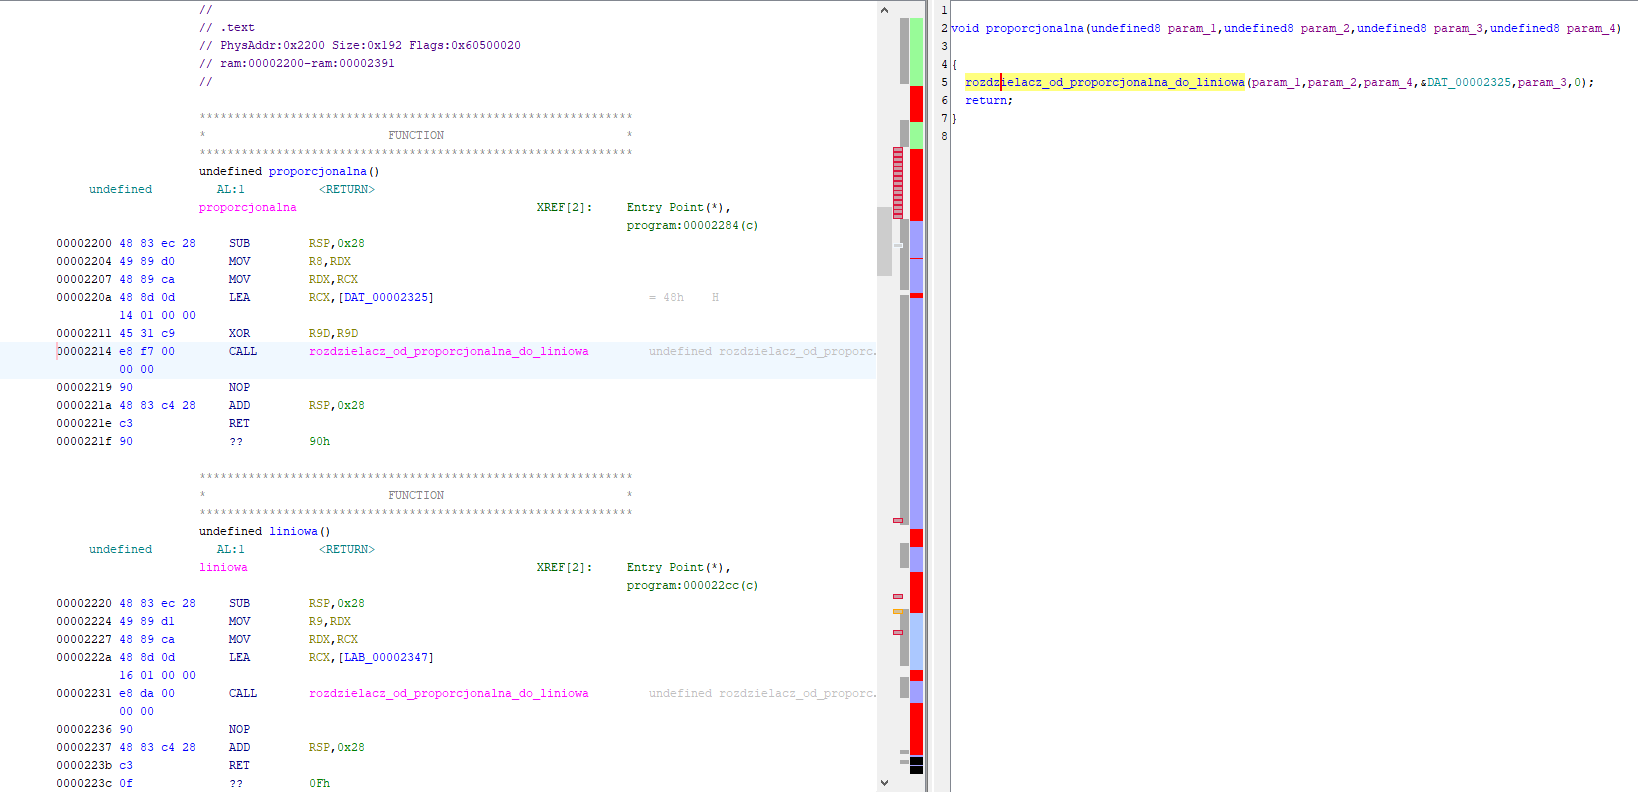
\includegraphics[width=1.2\textwidth]{images/2.rozdzielacz/1.png}
    \caption{Funkcja pośrednicząca}
\end{figure}
\FloatBarrier

Gdy jednak przejdziemy do funkcji rozdzielacza, zobaczymy, że dekompilator nie poradził sobie.
\begin{figure}[H]
    \centering
    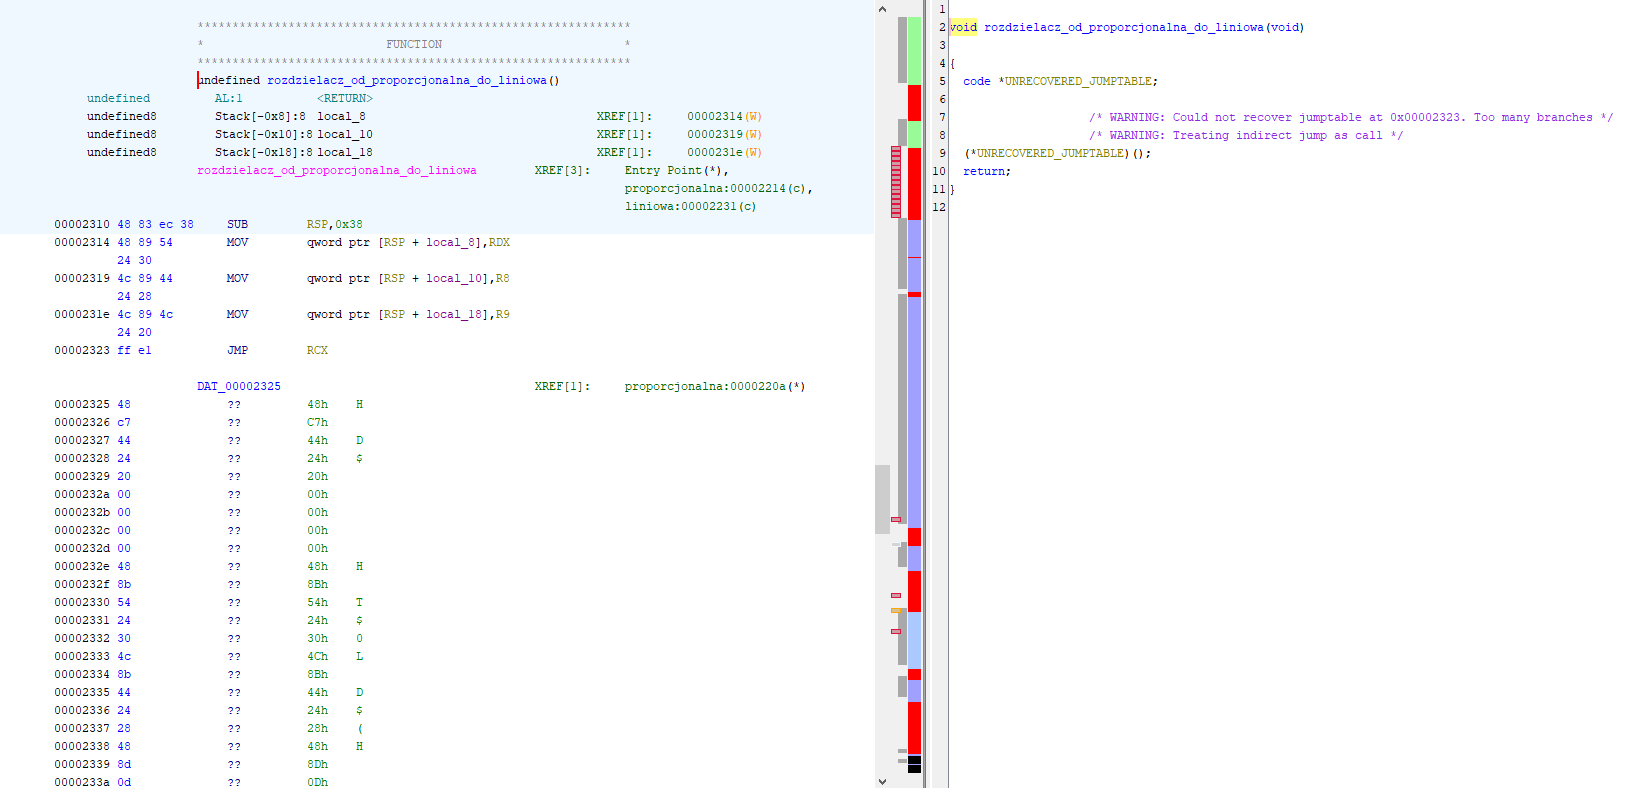
\includegraphics[width=1.2\textwidth]{images/2.rozdzielacz/2.png}
    \caption{Błędnie zdekompilowany rozdzielacz}
\end{figure}

Znajdująca się pod adresem 0002323 instrukcja JMP RCX jest poprawnym tłumaczeniem indirectbr \%0 - ,,skocz do adresu przekazanego w pierwszym parametrze'' w LLVM IR. Jednakże, dekompilator, natrafiając na skok pośredni, spodziewa się najwyraźniej, że jest to część tłumaczenia instrukcji switch i spodziewa się znaleźć tablicę skoków (której w tym wypadku nie potrzebujemy), stąd komunikat ,,Could not recover jumptable''. Nie możemy winić Ghidry za porażkę w tym wypadku, pokazaliśmy przecież wcześniej, że owej konstrukcji nie da się zapisać w C.

Możemy jednak uzyskać widok zdekompilowanego ciała funkcji, ręcznie podmieniając instrukcję - JMP RCX na JMP LAB\_00002325, czyli skok do następnego adresu (co dzieje się w jednej ze ścieżek wykonania programu). 
\FloatBarrier
\begin{figure}[H]
    \centering
    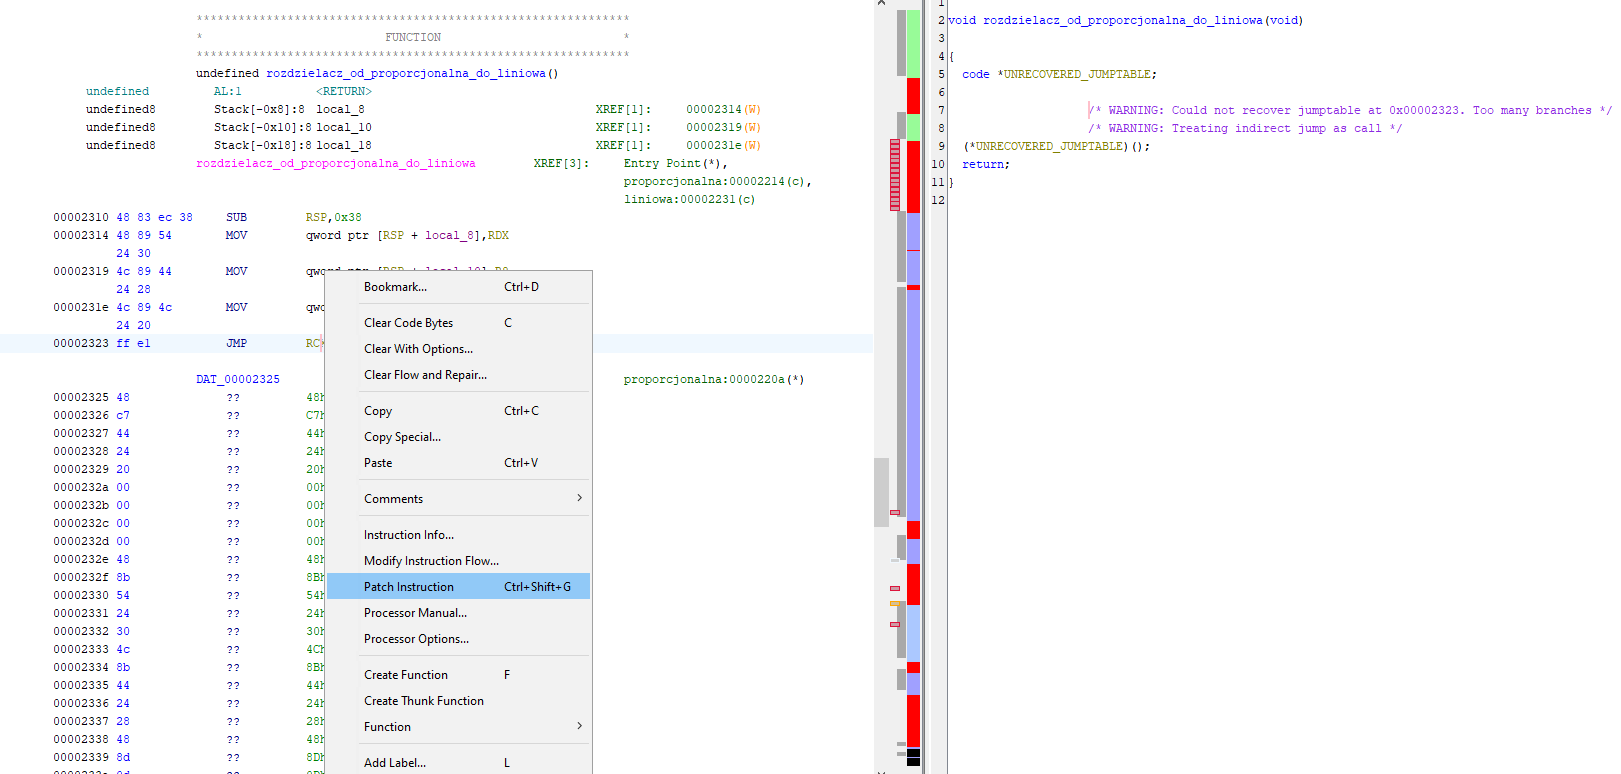
\includegraphics[width=1.2\textwidth]{images/2.rozdzielacz/3.png}
    \caption{Poprawianie pojedynczej instrukcji}
\end{figure}
Widzimy wtedy, że odtworzona została struktura procedury.
\begin{figure}[H]
    \centering
    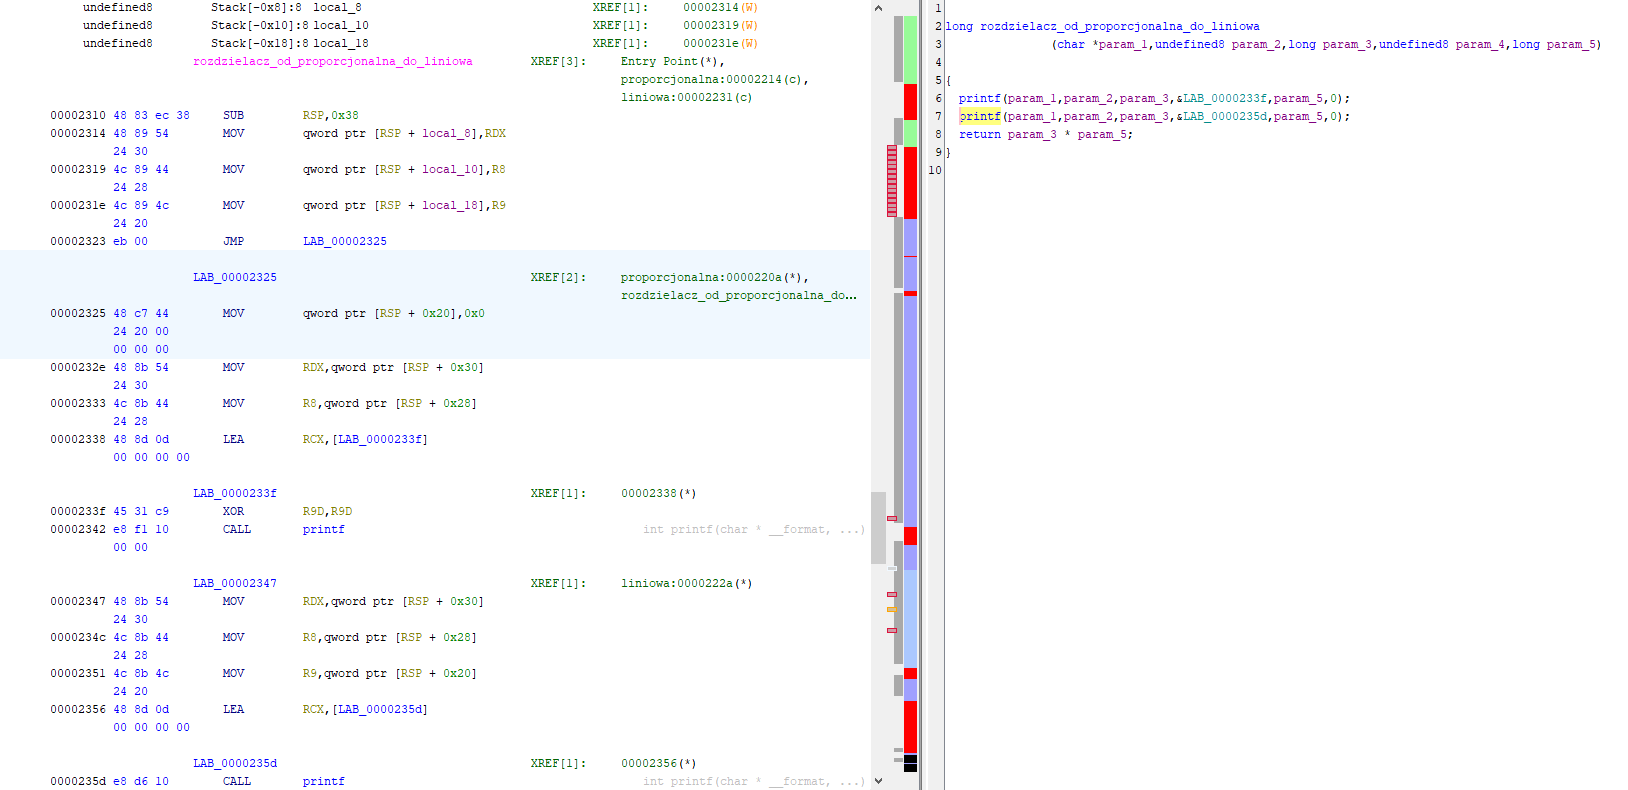
\includegraphics[width=1.2\textwidth]{images/2.rozdzielacz/4.png}
    \caption{Poprawnie zdekompilowany rozdzielacz po podstawieniu jednego z możliwych adresów w instrukcji skoku pośredniego}%%???
\end{figure}

Na sam koniec, sprawdźmy działanie programu (dodając odpowiednie przetwarzanie argumentów wywołania):
\begin{lstlisting}
printf(znak^,...)->całk32;
atoi(znak^)->całk32;
proc {
    zacznij proporcjonalna(całk a, całk x) -> całk;
    całk b=0;
    printf("\nproporcjonalna %lld %lld %lld",a,x,b);
    zacznij liniowa(całk a, całk b, całk x) -> całk;
    printf("\nliniowa %lld %lld %lld",a,x,b);
    zwróć a*x + b;
}
proc { zacznij program(całk argl, znak^^ argw) -> całk;
    całk zwr;
    jeśli(argl == 3)//a x
    {
        zwr = proporcjonalna(atoi(argw[1]), atoi(argw[2]));
    }
    inaczej{
        jeśli(argl == 4)
        {
            zwr = liniowa(atoi(argw[1]), atoi(argw[3]), atoi(argw[2]));
        }inaczej{printf("Zła liczba argumentów:%d a nie 2/3", argl-1); zwróć 0;}
    }
    printf("\nZwraca %d", zwr);
    zwróć 0;
}
\end{lstlisting}

Wywołajmy skompilowany program dwa razy, wchodząc do procedury pierwszym oraz drugim punktem wejściowym.
\begin{figure}[H]
    \centering
    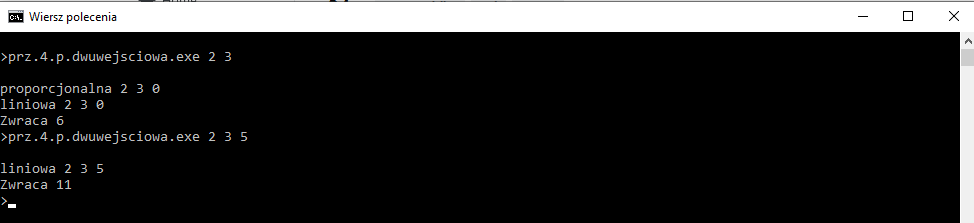
\includegraphics[width=1.0\textwidth]{images/2.rozdzielacz/cmdzrz.png}
    \caption{Dwukrotne wywołanie programu, testując oba punkty wejściowe}
\end{figure}

\section{Przenośność kompilatora}
Używając Javy, nie chciałem jednocześnie zależeć od konkretnego IDE, wybrałem więc Mavena do zarządzania projektem, da się bowiem cały proces budowania uruchomić za pomocą niego samego, z powłoki, powtarzalnie, z potencjałem do automatyzacji.. Wystarczy sklonować projekt z repozytorium i wykonać 'mvn clean install'. Przez wieloplatformowość Javy, oraz to że zależności - przede wszystkim antlr4, llvm i graphviz, są automatycznie pobierane z Sieci (nie jest wymagane instalowanie clanga w systemie), okazało się, że program kompilatora z minimalnymi zmianami w konfiguracji, da się również uruchomić na Linuksie. Rozmiar pobieranych pakietów pozostawia jednak w obecnej wersji wiele do życzenia.
%i to chyba tyle....
    \chapter{Wnioski}%%jeszcze niezbyt dokładnie zredagowane...
Napisanie programu prezentowanego kompilatora zajęło mi około trzech miesięcy wytężonej pracy w lecie 2024 roku. To niewątpliwie mniej niż osiemnaście roboczolat, zadeklarowanych przez twórców pierwszego kompilatora Fortranu\cite{FORTRAN_AUTOMATIC_CODING_SYSTEM}, czy czas spędzony na rozwoju Pascala\cite{Wirth_recollections_Pascal}. Nie jest to wynik zadziwiający, zważywszy na poziom rozwoju wykorzystanych narzędzi.

Zanim jednak ogłoszę możliwość nieskrępowanego praktykowania językotwórstwa eksploracyjnego w dzisiejszych warunkach, powinienem nadmienić, że całkowity koszt takiego projektu należałoby dość znacznie podwyższyć, o ile nie angażuje się w niego programistów posiadających już doświadczenie w tej dziedzinie. W moim wypadku, zdobycie tego doświadczenia oznaczało wpierw wykonanie wspomnianego projektu zaliczeniowego (który okazał się być o wiele bardziej pracochłonny, niż jest to właściwe). W następnych latach wykonałem również w zasadzie cztery aplikacje, wykorzystując pierwotny kod i pomysły i rozwijając umiejętności. Prezentowany tu program, jego architektura jest owocem tych wysiłków i wyciągania wniosków z różnorakich porażek (zwłaszcza związanych z pisaniem własnych maszyn wirtualnych). Proces projektowania języka wymagał dość szerokiej kwerendy, w celu przyswojenia i porównania istniejących rozwiązań, konieczne tez było przyswojenie literatury przedmiotu, w czym szczególnie pomocne okazał się być podręcznik Waite'a i Goos'a\cite{waite_goos} oraz ,,Dragon Book''\cite{DRAGON_BOOK}.

\subsection{Ortodoksja, heterodoksja i herezje}
W niniejszej pracy udało się zaprojektować nowy język wysokiego poziomu i wykonać jego kompilator. Język nie przystaje wprawdzie do stylu pojawiających się ostatnio języków programowania, ani do powszechnych poglądów na temat wykorzystywania języka polskiego w informatyce. Odbiega on jednak od ,,ortodoksji'' w granicach wyznaczonych przez wielkie dokonania lingwistyki formalnej, starsze języki (choć czerpiąc idee również ze współczesności), używając najnowszych narzędzi, mam zatem nadzieję, że nie popada w żadną ,,herezję'' i całe przedsięwzięcie można określić mianem ,,heterodoksyjnego''.

\subsection{Podobne projekty}
Nie jest to wprawdzie wiedza powszechna, sądząc po metrykach odwiedzin i reakcji, zapewnianych przez repozytoria, lecz istnieje obecnie dość dużo projektów o podobnej naturze, wykorzystujących LLVM. Jednymi z ciekawszych są Odin\cite{Odin} i jeszcze nie wydany Jai\cite{Jai}, mogące zapewniać miarę potencjalnych prospektów rozwoju (oraz trudności) dla prezentowanego projektu. Niektóre prezentowane w nich idee są niezwykle interesujące - np. ,,compile time execution'' z Jai można rozważać jako jedno z rozwiązań problemu zbytniego uogólniania języków ogólnego przeznaczenia i przesuwania analizy semantycznej do czasu wykonania, opisanej we wprowadzeniu (\ref{czy_potrzebne}).

\subsection{Możliwości rozwoju}
W tym wcieleniu projektu, udało się zaimplementować solidną, elastyczną ,,maszynerię'' kompilatora, pozostawiając sam język w dość podstawowej postaci. Powodem powstrzymania się od najciekawszej i najbardziej efektownej działalności językotwórczej była chęć uzyskania wpierw stabilnego systemu, aby zasadnicze błędy techniczne wyeliminować osobno, nie przeplatając ich z rozwojem mechanizmów translacji konstrukcji wysokopoziomowych. ,,Obniżanie'' konstruktów składniowych takich jak np. interfejsy czy ,,opasłe wskaźniki'' (fat pointers) wymaga znacznej ilości kodu (co można zaobserwować w repozytoriach) oraz wysiłku przeznaczonego na doprowadzenie ich do wymaganej niezawodności (co wybrzmiewa w komentarzach praktyków).

Z perspektywy prowadzenia projektu informatycznego, wydaje się być rozsądne, uzyskać wpierw solidny fundament, użytkować potem system w praktyce, celem zebrania doświadczeń, by dopiero potem przystąpić do następnego etapu. To powieszawszy, już mam przygotowany schemat translacji dla interfejsów, pewne modyfikacje inspirowane Swiftem oraz kilka innych pomysłów, które zamierzam zrealizować przy najbliższej okazji.
%%% do przepisania....

\subsection{Zakończenie}
Obserwując współcześnie rozwijane języki, nie sposób odnieść wrażenia, że żaden z nich nie może się obejść nie tylko bez oryginalnej nazwy, lecz i bez logotypu (często w formie animistycznej). Prezentowany tutaj język, z racji inspiracji wieloma językami z lat 70, których nazwy zaczynały się od PL/, oraz języka stanowiącego substrat leksykalny, otrzymał nazwę PL/PL oraz poniższy logotyp.

\begin{figure}[h]
    \centering
    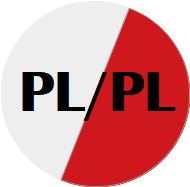
\includegraphics[width=0.3\textwidth]{images/znaczek.png}
\end{figure}
	
	% itd.
	% \appendix
	% \include{dodatekA}
	% \include{dodatekB}
	% itd.
	
	\printbibliography

\end{document}
